\documentclass{report} %article or report

\usepackage[margin=1in]{geometry}
\usepackage{nameref} % to get the name of the section to reference
\usepackage{hyperref} % hyperlinks to references
\usepackage{graphicx,caption} % Required for inserting images
\usepackage{placeins} % specify some float barrier for better float position
% \usepackage{float} % specifying image position?
\usepackage{xcolor} % For text colors
\usepackage{wrapfig}  % to wrap text around images
\usepackage[rightcaption]{sidecap}  % caption to the side of the image
% \usepackage{svg} % for .svg images this is actually not useful because it just converts it to pdf anyways
\usepackage{subfig} % for more figures together
\usepackage{amsmath} % math things ?
\usepackage[skip=10pt plus1pt, indent=0pt]{parskip}
\usepackage{titlesec} % improve chapter titles
% \usepackage{todonotes} % adds notes to the side, actually these slow down the compilation by a ton
\usepackage{tabularx}
% \usepackage{rotating}   % rotating tables? 
% \usepackage{lscape}    % rotating tables????
% \usepackage{adjustbox}  % I use it to rotate a table
\usepackage{makecell}  % to make two line elemenents in a cell
% \usepackage[symbol]{footmisc} % to use symbols for footnotes (https://tex.stackexchange.com/questions/826/symbols-instead-of-numbers-as-footnote-markers)
\usepackage{siunitx}  % SI units
\usepackage{derivative}
\usepackage[backend=biber, sorting=none, maxnames=2, style=ieee]{biblatex} %Imports biblatex package, style=nature/ieee/apsrev?
\usepackage{tablefootnote}  % footnotes in tables don't appear otherwise
\usepackage{lineno}  % line numbers
\linenumbers

% \usepackage{biblatex} %Imports biblatex package
%THIS TO INCLUDE THE VAVILOV_LANDAU LATEX FILE
% \usepackage{Vavilov_packages}

% \newcommand{\specialcell}[2][c]{%
%   \begin{tabular}[#1]{@{}c@{}}#2\end{tabular}}
\DeclareSIUnit{\barn}{b}
\DeclareSIUnit{\neutroneq}{n_{eq}}

\newcommand{\captionwidth}{.9\linewidth}

%%% trying to adjust floats settings
\renewcommand{\topfraction}{.85} % .7
\renewcommand{\bottomfraction}{.7} % .3
\renewcommand{\textfraction}{.15} % .2
\renewcommand{\floatpagefraction}{.66} % .5
% \renewcommand{\dbltopfraction}{.66} % .7
% \renewcommand{\dblfloatpagefraction}{.66} % .5
\setcounter{topnumber}{9} % 2
\setcounter{bottomnumber}{9} % 1
\setcounter{totalnumber}{20} % 3
% \setcounter{dbltopnumber}{9} % 2
\setlength{\floatsep}{4pt}

\hypersetup{
    colorlinks,
    citecolor=black,
    filecolor=black,
    linkcolor=black,
    urlcolor=black
}

\addbibresource{bibliography.bib} %Import the bibliography file
\setlength\bibitemsep{\baselineskip}


\title{Test Beam analysis for HGTD}
\author{Marcello Pozzessere}
\date{January 2025}

\begin{document}

\maketitle
% \renewcommand{\thesection}{\arabic{section}}
% \titleformat{\chapter}{\bfseries\huge}{\thechapter.}{20pt}{\huge\it}
\titleformat{\chapter}[hang]{\Huge\bfseries}{\thechapter\,\textcolor{gray}{|}\,}{0pt}{\Huge\bfseries}

\tableofcontents


\chapter*{Introduction}\label{chap:intro}
\addcontentsline{toc}{chapter}{\nameref{chap:intro}}

%%%     - LHC high lumi, pileups in ATLAS
%%%     - HGTD and LGADs 
In the coming years, the LHC will undergo a series of upgrades to accommodate the requirements of the High-Luminosity phase~\cite{cernHLLHCProject}, aimed at enabling more precise measurements and improving sensitivity to rare processes beyond the Standard Model.

In particular, the ATLAS experiment will have many of its subdetectors improved and/or replaced. Additionally, to help deal with the problems caused by the increased luminosity, a new detector system will be integrated into the experiment: the High Granularity Timing Detector~\cite{cernTechnicalDesign}. The HGTD will provide time information of charged particles, helping differentiate between collisions that happen very close in space but well separated in time. To achieve this, a special type of silicon sensors will be employed: Low Gain Avalanche Detectors~\cite{PELLEGRINI201412}. These sensors combine very fast response with an internal gain, to enhance the signal and better endure the high radiation environment that they will face.

%%%     - LGADs requirements
%%%     - test beam
To achieve the HGTD's precision targets, the LGADs need to satisfy some requirements. The sensors must collect enough charge for the signal to be measured by the electronics (\(\approx \qty{4}{\femto\coulomb} \)), they must have a time resolution better than \qty{35}{\pico\second} at start of life (and up to \qty{70}{\pico\second} at end of life), and, finally, they must have an efficiency per hit greater than \(95\%\).

There exist several vendors and version of LGADs so, to test and compare their perfomances, the sensors are typically put through a collimated beam of accelerated particles, simulating the environment of the ATLAS detector. In this thesis we focused on the test beam campaign of May 2023, conducted at one of CERN's facilities, where LGADs from three different vendors were characterized: USTC (University of Science and Technology of China), IHEP (Institute of High Energy Physics, China) and CNM (Centro Nacional de Microelectr\'onica, Spain).

A telescope of 6 silicon pixel detectors was used for track reconstruction, a cooling box maintained the LGADs at \qty{-30}{\degreeCelsius} and another device had the role of reference for the time resolution measurements. 

%%% methods overview
After some pre-processing, the data was further refined to avoid various sources of noise. For each sensor, the time resolution, the collected charge and the efficiency were calculated. The sensors were grouped based on version, vendor and level of radiation for easier comparison. Additionally, some interesting effects that emerged during the analysis were further investigated.

%%% Thesis structure (optional)
The first \hyperref[chap:LHC_ATLAS]{chapter} of this thesis describes in general the LHC and the ATLAS experiment, the \hyperref[chap:HGTD_LGADs]{next chapter} focuses on the HGTD and the silicon sensors it will use: the LGAD. The \hyperref[chap:testbeam_setup]{following chapter} describes the key elements in the test beam setup used for taking data. The \hyperref[chap:analysis]{fourth chapter} follows the implementation of the analysis, providing the reasons and the tools used. Finally, the \hyperref[chap:results]{fifth chapter} presents the general results of the analysis. Some additional information, plots and tables are provided in the Appendix.



%%% intro on CERN and LHC 
%%% goals of particle physics research at CERN

\chapter{The LHC and the ATLAS experiment}%\label{chap:LHC_ATLAS}

The theory that currently best describes the fundamental particles and their interactions is known as the Standard Model \cite{Herrero1999}. It was developed during the 20th century and finalized in the mid-1970s, after experimenal confirmations of quarks. The Standard Model has since predicted and explained a wide range of phenomena with great accuracy, important examples are the W and Z bosons and the Higgs boson. However, some questions still remain unanswered.


\section{The Large Hadron Collider}
\begin{figure}[!ht]
    \centering
    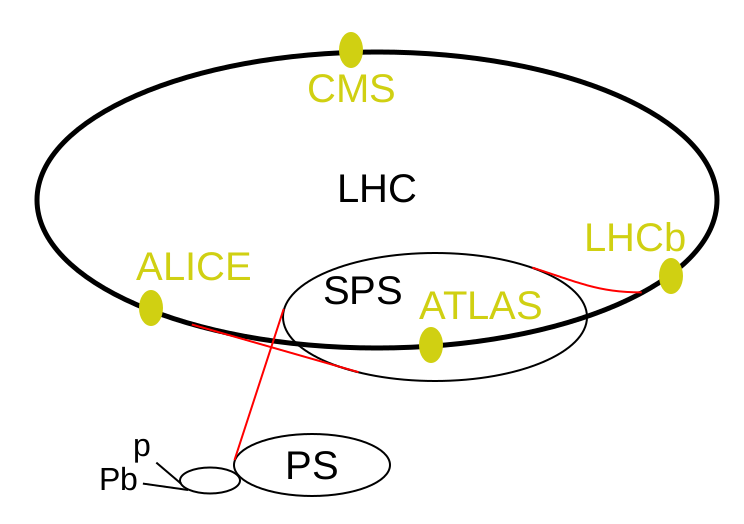
\includegraphics[width=.7\linewidth]{Images/intro/LHC.png}
    \captionsetup{width=.7\linewidth}
    \caption{Simplified scheme of the CERN accelerator complex. Each proton or lead ion starts from a linear accelerator (LINAC 4 and LINAC 3, respectively, not in the picture), it is then transferred to the Proton Synchrotron (SP), into the Super Proton Synchrotron (SPS) and finally into the Large Hadron Collider (LHC). During each phase of acceleration the particles reach higher momentum before being transferred to the next stage.}
    \label{fig:LHC}
\end{figure}

\marginpar{\flushleft I could add some details of the process of acceleration, from H atoms to proton beam into the LHC}

The Large Hadron Collider (LHC) is the largest particle accelerator in the world. It was built between 1998 and 2008 by the European Organization for Nuclear Research (CERN, \textit{Conseil européen pour la Recherche nucléaire}) in collaboration with more than 100 countries with the purpose of colliding hadrons\footnote{\label{footnote:hadrons}Hadrons are particles that are made up of two or more quarks, e.g. protons and neutrons} at high energies and study the products of these collisions. It consists of a \qty{27}{\kilo\meter} ring at roughly \qty{100}{\meter} of depth situated at the Franco-Swiss border, near Genève. Two beams of particles travel at near light speed in opposite directions inside two pipes surrounded by superconducting magnets. At specific locations the beams converge and collisions take place, these events can then be observed with specialized detectors built along the ring.


\subsection{The research goals}%\label{sec:CERN_research_goals}

The construction of the LHC was motivated by the need for experimental data to study the laws of our universe. In particular, its main objectives were \cite{homeFactsFigures}:
\begin{itemize}
    \item The search for the Higgs boson: the particle (whose mass could not be predicted) responsible for the origin of mass, culminated in the discovery of the Higgs boson in 2012 \cite{ATLAS:2012yve}. 
    \item Supersymmetry: a theory that hypothesizes the existence of massive partners of the particles in the current Standard Model.
    \item Dark matter and dark energy: the matter that we know only makes up a small fraction, $\sim$4\%, of the content of the universe, and the particles or phenomena responsible for the remaining 23\% (dark matter) and 73\% (dark energy) are still unknown.
    \item Matter-antimatter asymmetry: matter and antimatter should have been produced in equal amounts during the Big Bang, yet observations show an overwhelming prevalence of normal matter.
    \item Quark-gluon plasma: a state of matter that existed in the early stages of the Universe, before ordinary matter could emerge.
\end{itemize}

The LHC is part of the CERN accelerator complex, a chain of machines in which each link accelerates a beam of particles (protons or heavy ions) to higher energies and feeds it to the next one. A simplified version of the complex is shown in Figure \ref{fig:LHC}. The LHC began operations in 2010 with energies of \qty{3.5}{\tera\electronvolt}, increased up to \qty{4}{\tera\electronvolt} in 2012. After two years of Long Shutdown for upgrades and maintenance, activities resumed in 2015 with Run 2, and beam energies of \qty{6.5}{\tera\electronvolt} ($\sqrt{s}=\qty{13}{\tera\electronvolt}$, center of mass energy) were achieved.


\subsection{The main experiments}\label{subsec:LHC_main_experiments}

Along the accelerator tracks there are four main experiments (Figure \ref{fig:LHC}):
\begin{itemize}
    \item ALICE (A Large Ion Collider Experiment): dedicated to heavy-ion physics~\cite{aliceFrontpageAlicepublicwebcernch}.
    \item ATLAS (A Toroidal LHC Apparatus): one of the two general-purpose detectors, able to investigate a wide range of physics~\cite{atlasATLASExperiment}.
    \item CMS (Compact Muon Solenoid): the second general-purpose detector of LHC~\cite{cmsDetectorExperiment}.
    \item LHCb (Large Hadron Collider beauty): an asymmetric detector that observes mainly forward particles to study the "b quark"~\cite{cernLHCbCollaboration}.
\end{itemize}

Additionally, there are several other experiments part of the CERN complex, including test beam facilities in the North Area which use particle beams from SPS to perform a variety of tests.

\begin{figure}[!ht]
    \centering
    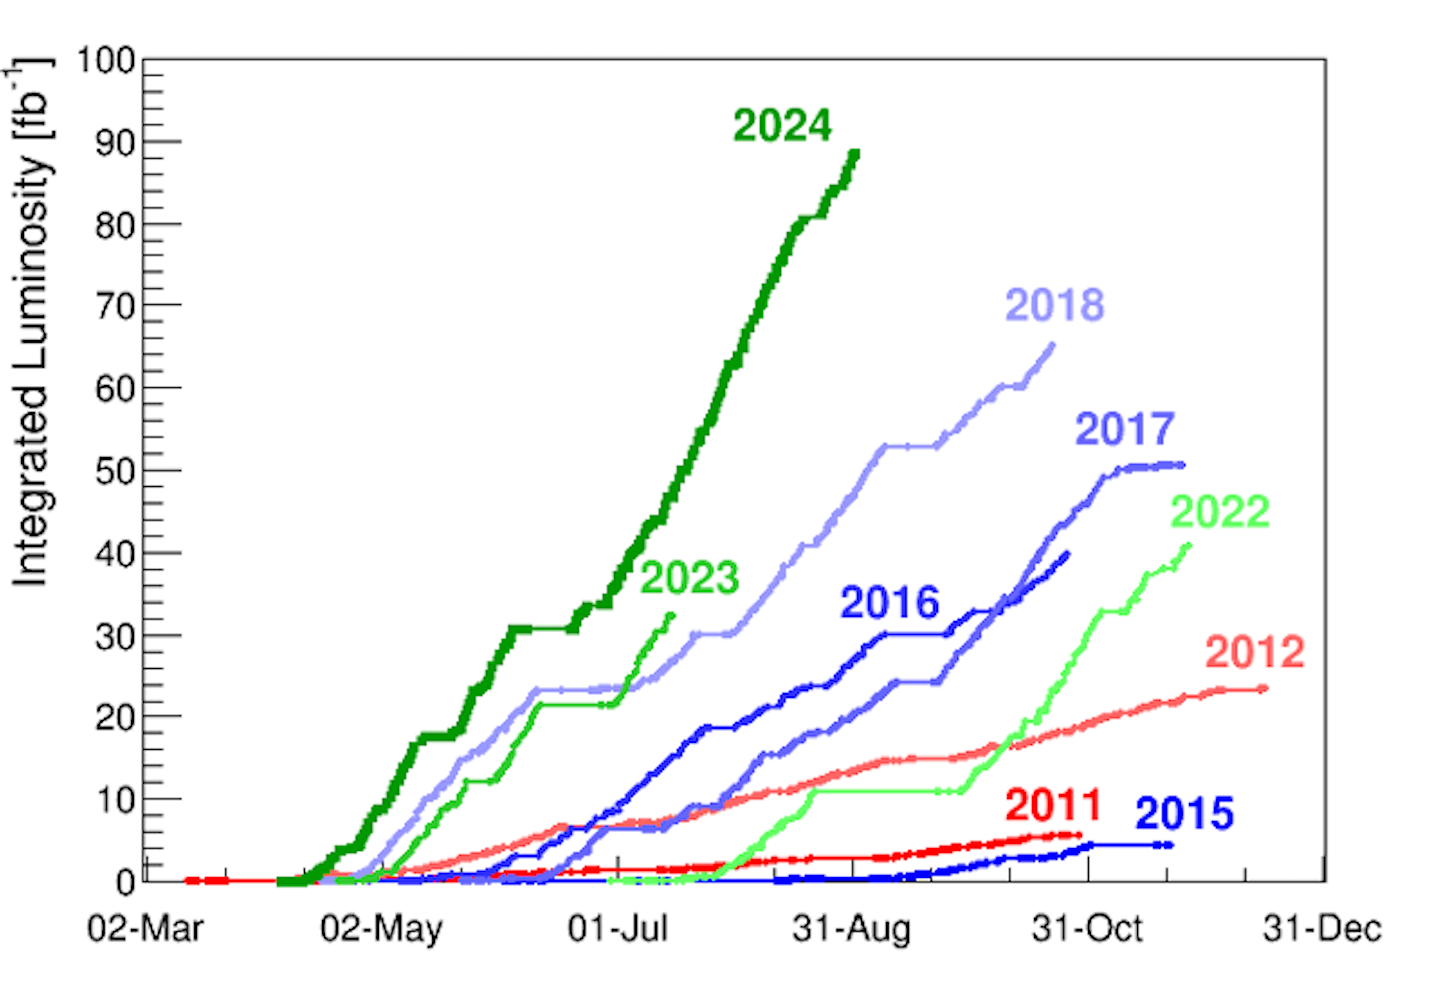
\includegraphics[width=.6\linewidth]{Images/intro/integrated_luminosity.png}
    \captionsetup{width=.8\linewidth}
    \caption{Overview of the integrated luminosity as a function of the date for each year of LHC running, with 2024 greatly exceeding all other years. From \cite{homeAcceleratorReport}.}
    \label{fig:integrated_luminosity}
\end{figure}

One of the most important parameters of a collider, along with the beam energy, is the luminosity. It is used to quantify the amount of interactions that will occur and, therefore, the expected rate of events produced by the collisions. For two bunches\footnote{\label{footnote:particle_beam_bunches} The particles in the LHC beam do not travel uniformly distributed, rather they are grouped in many \textit{bunches}, synchronized to intersect at the center of each main detector% (Section \ref{subsec:LHC_main_experiments}) %%% it's in the same Section
.} colliding head-on with frequency $f_{coll}$, the luminosity can be calculated by:

\begin{equation}
    \mathcal{L} = f_{coll}\frac{N_1 N_2}{4\pi \sigma_x \sigma_y} \mathcal{F} \, \left[\unit{cm^{-2}.s^{-1}}\right] \, .
\end{equation}

Where $N_1$ and $N_2$ are the number of particles in each bunch, $\sigma_x$ and $\sigma_y$ define the transverse spread of the bunches (approximately normal distributions) at the interaction point, and $\mathcal{F}$ is a factor of order $1$ to account for inefficient geometric overlapping and other effects.

A related quantity is the integrated luminosity, which is the integral over time of the instantaneous luminosity. It quantifies the amount of data that is available to be studied, and it is typically measured in inverse femtobarns \unit{\femto\barn^{-1}}=\qty{e-28}{\meter^{-2}}.

After the second Long Shutdown that took place between 2018 and 2022 LHC has been operating (Run 3) and already delivering record breaking integrated luminosity (Figure \ref{fig:integrated_luminosity}).

%%% plans for the next years
\subsection{High-Luminosity upgrade}\label{subsec:high_luminosity_upgrade}
In the upcoming years there will be a third Long Shutdown (from around 2026,until early 2029) to prepare for the next phase: the High-Luminosity LHC Project (HL-LHC) \cite{cernHLLHCProject}. The plan aims to increase the instanteous luminosity up to \qty{1.5e34}{\centi\meter^{-2}\second^{-1}} (compared to \qty{2.1e34}{\centi\meter^{-2}\second^{-1} of Run 2} \cite{CERN-LHCC-2020-007}) and to bring the integrated luminosity up to \qty{3000}{\femto\barn^{-1}} in the following 10-12 years. This will enable more accurate measurements of new particles and the possibility to observe rare processes below the current sensitivity level. On the other hand, this upgrade will introduce a wide range of new challenges for all the systems within CERN's accelerator complex. For instance, the detectors will be exposed to higher radiation doses, which may impact performance, and the increased number of collisions will lead to more pronounced pile-up effects complicating track reconstruction.

% this is already kinda talking about HGTD, maybe it's a good bridge to the next section: HGTD
\begin{figure}[!ht]
    \centering
    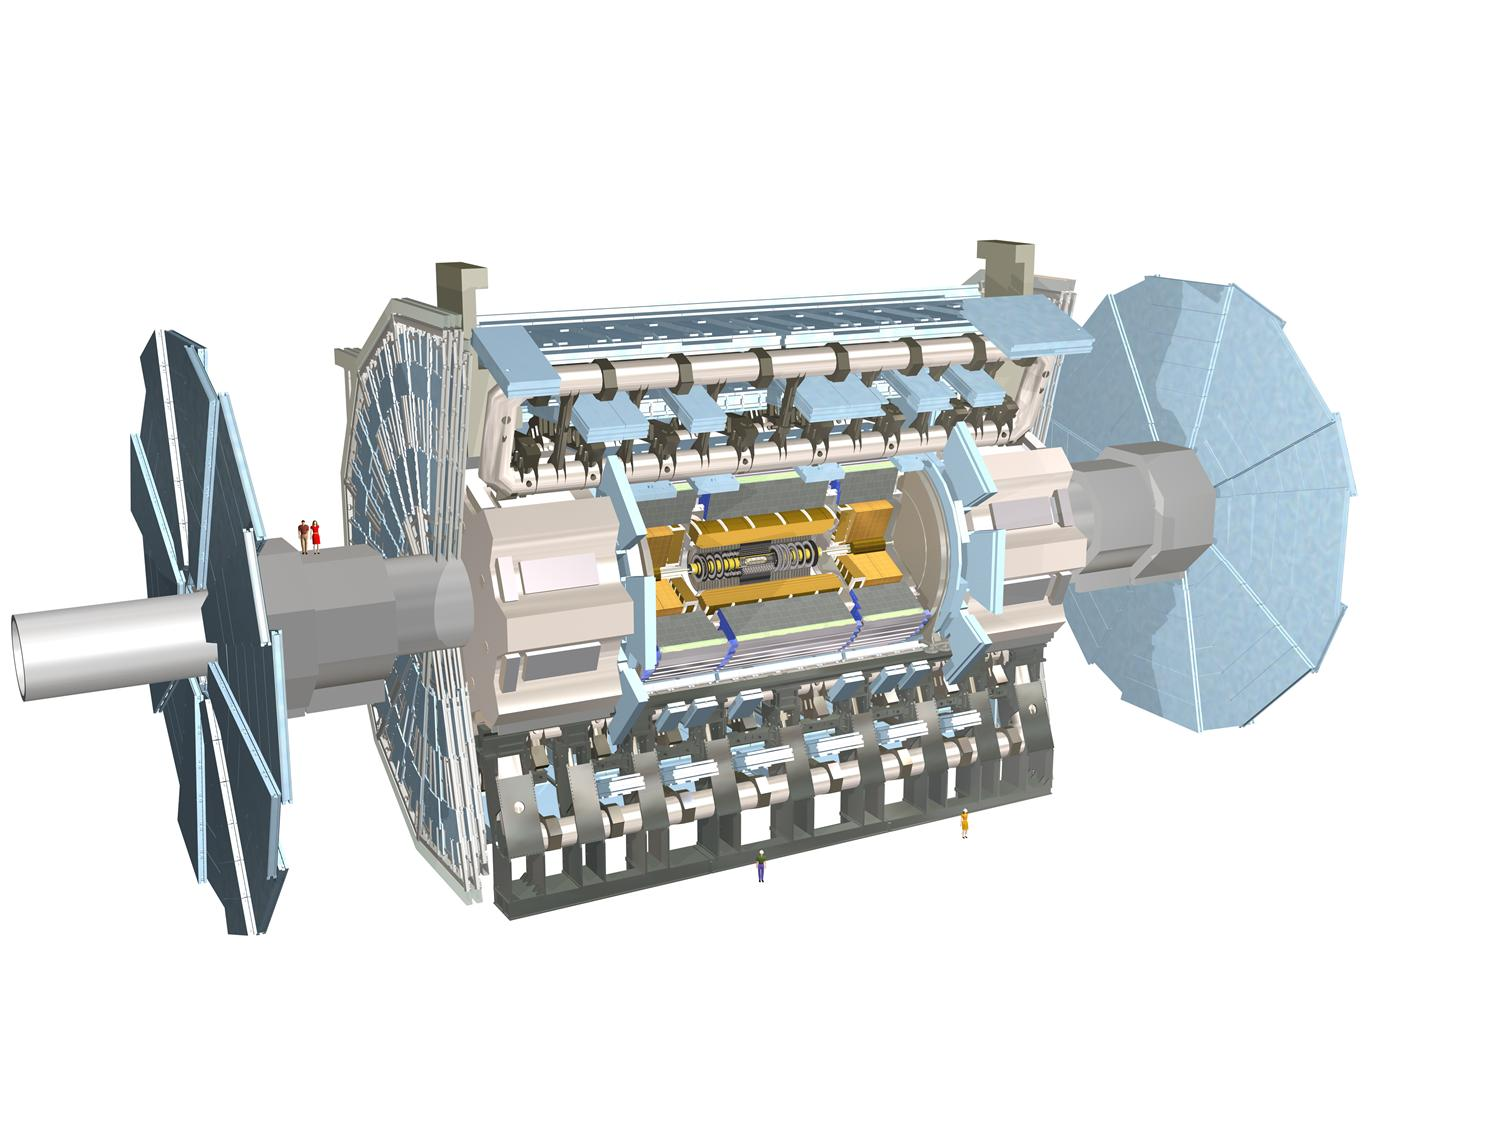
\includegraphics[width=.7\textwidth]{Images/intro/ATLAS_detector.jpg}
    \captionsetup{width=.8\linewidth}
    \caption{Overview of the ATLAS detector. From \cite{atlasDetectorTechnology}}
    \label{fig:ATLAS}
\end{figure}


\section{The ATLAS experiment}%\label{chap:ATLAS}

ATLAS (\textbf{A} \textbf{T}oroidal \textbf{L}HC \textbf{A}pparatu\textbf{S}) is a general purpose detector built for probing \textit{p-p} and \textit{A-A} collisions (\textit{proton-proton} and \textit{heavy ion-heavy ion}, respectively). Currently, the experiment's main detector systems are: the Inner Detector, the Calorimeters, the Muon Spectrometer and the Magnet System \cite{Collaboration_The_ATLAS2008}. 

\begin{figure}[ht]
    % \centering
    % \subfloat[Radial view of the ATLAS Inner Detector. From \cite{atlasInnerDetector}]{
    %     \includegraphics[width=.48\linewidth]{Images/intro/ATLAS_inner_detector_radial_description.jpg}
    %     \label{fig:ATLAS_inner_detector_radial}}
    % \hfill
    \centering
    \subfloat[The Inner Detector and its three components: the Pixel Detector, the Semiconducor Tracker and the Transition Radiation Tracker. From \cite{atlasInnerDetector}.]{
        \includegraphics[width=.45\linewidth]{Images/intro/ATLAS_inner_detector.jpg}
        \label{fig:ATLAS_inner_detector}}
    \hfill
    \centering
    \subfloat[The Calorimeters: the Liquid Argon Calorimeter (LAr), comprising the barrel, electromagnetic and hadronic end-cap, and foward sections, and the Tile Hadronic Calorimeter, divided into barrel and extended barrel sections. From \cite{atlasCalorimeter}.]{
        \includegraphics[width=.45\linewidth]{Images/intro/ATLAS_calorimeter_description.jpg}
        \label{fig:ATLAS_calorimeter}}
    \caption{Cutaway views of the ATLAS Inner Detector (left) and Calorimeter system (right).}
\end{figure}


\subsection{Inner Detector}\label{sec:ATLAS_inner_detector}
\marginpar{\flushleft }
The main purpose of the Inner Detector is to reconstruct the verteces of the collisions, it comprises three sub-detectors (Figure \ref{fig:ATLAS_inner_detector}).

The Pixel Detector is the first point of detection, only \qty{3}{\centi\meter} away from the LHC beam line and it is made of four layers of silicon pixels, more than 92 million in total. Charged particles originated from the collision points leave a small amount of energy that can be measured by the pixels with a precision of almost \qty{10}{\micro\meter}. These signals are then used to reconstruct the origin and the momentum of the particles.

The Semiconductor Tracker surrounds the Pixel Detector and complements it in the detection and reconstruction of the tracks of charged particles. It consists of over 6 million "micro-strips" silicon detectors with a precision of up to \qty{25}{\micro\meter}.

The final layer of the Inner Detector is the Transition Radiation Tracker (TRT). Unlike its neighbouring silicon sub-detectors, TRT is composed of \num{300000} \qty{4}{\milli\meter} diameter tubes with a \qty{30}{\micro\meter} gold-plated tungsten wire in the centre and filled with a mixture of gas. As charged particles pass through the volume they ionize the gas, which creates detectable electric signals. The location can then be determined, helping with the tracks reconstruction and the momentum measurement. Additionally, the moving particles emit transition radiation\footnote{Transition Radiation occurs when a charged particle traverses materials with different refraction index, such as the boundary between two different media \cite{wikipediaTransitionRadiation}.}, and the intensity of this radiation depends on the $\gamma$ Lorentz factor, thus allowing to distinguish between heavier and lighter particles.


\subsection{Calorimeter}\label{sec:ATLAS_calorimeter}

% \begin{figure}[!ht]
%     \centering
%     \includegraphics[width=.8\textwidth]{Images/intro/ATLAS_calorimeter_description.jpg}
%     \captionsetup{width=.8\linewidth}
%     \caption{Layout of the components inside the Calorimeter. From \cite{atlasCalorimeter}}
%     \label{fig:ATLAS_calorimeter}
% \end{figure}

Calorimeters are designed to absorb most of the incoming particles, forcing them to deposit all of their energy and stop within the detector. They are divided into two categories: electromagnetic and hadronic calorimeters. Electromagnetic calorimeters (ECAL) measure the energy of electrons and photons while they interact with matter via electromagnetic force. Hadronic calorimeters, on the other hand, measure the energy of hadrons\footref{footnote:hadrons} as they interact with atomic nuclei via strong force. Calorimeters can stop most known particle, with the exception of muons\footref{footnote:muons} (observed with \ref{sec:muon_spectrometer}) and neutrinos.

The ATLAS calorimetry system uses two different technologies: the Liquid Argon Calorimeter (LAr) and the Tile Hadronic Calorimeter.

The Liquid Argon Calorimeter (LAr) features layers of metal (either tungsten, copper or lead), with liquid argon in-between, kept a temperature of \qty{-184}{\degreeCelsius}. Several modules are placed cylindrically around the beam (the barrel) and at the extremities (endcaps). The LAr forward (FCal) covers the region close to the beam using three disks of metal (copper, tungsten and tungsten).

The Tile Hadronic Calorimeter surrounds the LAr calorimeter, it has the goal of measuring hadronic particles that did not deposit all of their energy in the LAr. It consists of alternating layers of steel and plastic scintillating tiles. Particles hitting the steel layer create a shower of other particles, the plastic scintillators in turn produce photons, which are then converted into an electric current to determine the original particle's energy.

\subsection{Muon Spectrometer}\label{sec:muon_spectrometer}

The outer layer of the ATLAS experiment is composed of muon\footnote{Muons are particles similar to electrons but $\sim$200 times heavier. This allows them to penetrate much deeper into matter, due to less emitted radiation as they decelerate. \label{footnote:muons}} detectors, which identify and measure the momenta of muons. It employs several detector technologies separated into two categories: Fast-Response Detectors, to quickly select collisions potentially interesting for physics, and Precision Detectors, to provide very precise positions of muons.

In the first group there are: 
\begin{itemize}
    \item Resistive Plate Chambers (RPCs): gaseous detectors surrouding the central region of ATLAS. They are pairs of parallel plates at an electric potential difference, separated by gas.
    \item Thin Gap Chambers (TGCs): wire-based gas detectors found at the ends of ATLAS, consisting of \qty{30}{\micro\meter} parallel wires in a gas mixture.
\end{itemize}
Both of these detectors measure the electric signals of particles as they ionize the gas.

Finally, for the role of Precision Detectors, Monitored Drift Tube (MDTs) are able to determine the position of a muon to an accuracy of \qty{100}{\micro\meter}. They are consituted by more than \num{380000} aluminium tubes with a wire at the tube's center and filled with a gas mixture. They are stacked up over several layers, to precisely trace the path of each muon.


\subsection{Magnet System}\label{sec:magnet_system}

\begin{figure}[!ht]
    \centering
    \subfloat[The Central Solenoid Magnet at its installation, 2004. From \cite{atlasMagnetSystem}.]{
        \includegraphics[width=.45\linewidth]{Images/intro/ATLAS_central_solenoid_magnet.JPG}
        \label{fig:ATLAS_central_solenoid}}
    \hfill
    \centering
    \subfloat[The installation of the eighth and final coild of the Barrel Toroid Magnet, 2005. From \cite{atlasMagnetSystem}.]{
        \includegraphics[width=.45\linewidth]{Images/intro/ATLAS_barrel_toroid_magnet.JPG}
        \label{fig:ATLAS_barrel_toroid}}
    \caption{Photos of ATLAS magnets during their installation.}
\end{figure}

Powerful magnets are used to bend the trajectories of charged particles, enabling the measurement of their momentum and charge. In ATLAS this is done two different types of superconducting magnet systems: toroidal and solenoidal, utilized in the three main sections: Central Solenoid Magnet, Barrel Toroid and End-cap Toroids.
\begin{itemize}
    \item Central Solenoid Magnet: surrounds the inner detector at the core of ATLAS. It provides a \qty{2}{\tesla} magnetic field in just \qty{4.5}{\centi\meter} thickness (Figure \ref{fig:ATLAS_central_solenoid}).
    \item Barrel Toroid: the largest toroidal magnet ever constructed, providing a magnetic field of up to \qty{3.5}{\tesla}. It is used to measure the momentum of muons.
    \item Two End-cap Toroids: placed at each end of the experiment, extending the magnetic field to deflect particles escaping the detector along the beam pipe.
\end{itemize}

\subsection{ATLAS upgrades}\label{subsec:ATLAS_upgrades}

As part of the \nameref{subsec:high_luminosity_upgrade}, the ATLAS detector will undergo several changes, including \cite{MANGHI2024169917}: %% (not exhaustive)

\begin{itemize}
    \item Inner Tracker (ITk): a new all-silicon tracker will replace the \nameref{sec:ATLAS_inner_detector}. It will be composed of outer Si strip sensors (4 barrel layers and 6 end-cap disks) and inner Si pixel sensors (5 barrel layers and end-cap rings). The new pixel system will cover an area of about \qty{13}{\meter^2}, a significant increase compared to \qty{1.9}{\meter^2} of the current pixel detector. The pseudorapity range will also increase from $\eta=2.5$ to $\eta=4$ \cite{Buttar:2024imj}.
    \item Calorimeter electronics: both calorimeters will see the replacement of all electronics to comply with a new Trigger and Data Acquisition architecture, which will provide improved precision and granularity. 
    \item Muon spectrometer: two new chamber technology systems \cite{2106380} will be installed on the New Small Wheel \cite{Kawamoto:2013udg}. Micromegas (MicroMEsh GAseous Structure), which will serve as primary tracking detector, and Small-Strip Thin-Gap Chambers (sTGCs), which will function as primary trigger detector.
    \item HGTD: a new silicon pixel detector that will provide timing information in the forward region, to improve vertex reconstruction. The design of the detector and its modules are described in more detail in the next chapter (\nameref{chap:HGTD_LGADs}.)
\end{itemize}

\marginpar{\flushleft there is also LUCID-3 in \cite{MANGHI2024169917}, PMTs for luminosity measurements.}

%%% what LGADs are
%%% working principles
%%% requirements for the detector
%%% other studies 
%%% expected results
\chapter{HGTD and LGADs}\label{chap:HGTD_LGADs}

%%% I have to put an actual "summary" of the chapter
% In this chapter we motivate the construction of HGTD, illustrate its general layout and describe the specific type of silicon sensors (LGADs) that constitute the active components of the detector.
The upcoming High-Luminosity phase has the goal of increasing the integrated luminosity by a factor \(10\), enhancing the potential of new physics discoveries. However, it will also bring a variety of new complications, most importantly the increase in pileup interactions\footnote{Multiple collisions happening during the same bunch crossing, on top of a main event of interest.}.
%%% HGTD as a solution 
A new way to mitigate this effect for higher pseudorapidity values will be "\textit{to use high-precision timing information to distinguish between collisions occurring very close in space but well-separated in time}" \cite{CERN-LHCC-2020-007}. This is set to be accomplished by the High Granularity Timing Detector (HGTD).
The HGTD will improve the object reconstruction capabilities of ATLAS, complementing the ITk. This, in turn, will help study a variety of processes that rely on the precise identification and measurement of the physics objects produced during \(p-p\) collisions, such as jets and leptons.
The detector's active elements will be silicon sensors, which will provide precise timing information and will withstand the additional radiation of the HL. To achieve the HGTD's preicison goal of \qty{30}{\pico\second} (\qty{50}{\pico\second}) at start life (end life), the sensors will need to have a time resolution per hit of \qty{35}{\pico\second} (\qty{70}{\pico\second}). Additionally, a hit efficiency above \(95\%\) and %a due to the electronics' spefications,
a minimum collected charge of \qty{4}{\femto\coulomb} will also be required.
% I need to add the sensor requirements: time resolution, charge and efficiency 

In this chapter we describe the general design of the HGTD, its benefits to object reconstruction and the special type of silicon sensors (LGAD) that will form its basic components.

\section{The High Granularity Timing Detector}\label{sec:HGTD}
%%% ITk
One of the updates to the ATLAS detector will be the installation of the new ITk, which will improve the tracking\footnote{Tracking refers to the process of reconstructing the paths of charged particles as they fly through a detector. From the curvature of the track the momentum and the charge can be inferred. It is a fundamental part of event reconstruction.} and will extend the pseudorapidity range up to \(\eta=4\). While this extension will improve the reconstruction of physics objects, it will bring some difficulties too.

%%% event reconstruction
Event reconstruction relies strongly on the precise assignment of a track to the location of the first collision (primary vertex). % (track-to-vertex association).
Generally, a track is associated to a vertex if the track's origin is compatible with the vertex, this compatibility can be determined with:

\begin{equation}\label{eq:compatibility_vertex}
    \frac{\left|z_0 - z_{vertex}\right|}{\sigma_{z_0}} < s \,.
\end{equation}
 
Where \(z_0\) is the longitudinal impact parameter, \(z_{vertex}\) is the vertex position, \(\sigma_{z_0}\) is the spacial resolution and \(s\) is a significant cut (typically 2.5 or 3)\cite{cernTechnicalDesign}. 

\begin{figure}[h!tbp]
    \centering
    \subfloat[Simulation of the local pileup vertex densities for two values of \(<\mu>\) (average number of collisions per bunch crossing), indicative of the current and future collision rates. From~\cite{cernTechnicalDesign}.]{
        \includegraphics[width=.45\linewidth]{Images/intro/pileup_density_simulation.png}
        \label{fig:pileup_densities}}
    \hfill
    \centering
    \subfloat[Simulation of the longitudinal resolution of the ITk as a function of \(\eta\), for muons with \(p_T=\qty{1}{\giga\electronvolt}\) and \(p_T=\qty{10}{\giga\electronvolt}\) From~\cite{cernTechnicalDesign}.]{
        \includegraphics[width=.46\linewidth]{Images/intro/ITk_z_resolution_for_eta.pdf}
        \label{fig:ITk_spacial_resolution}}
    \caption{Simulations of the pileup densities (left) and the ITk spacial resolution (right).}
\end{figure}

%%% difficulties/problems
Some problems arise. 
Firstly, as \(\eta\) increases, tracks become more parallel to the beam and are subject to multiple scattering effects due to more material compared to the central barrel region. Secondly, the HL-LHC will see a rise in the number of collisions per bunch %\footref{footnote:particle_beam_bunches} %%% this footnote is from the previous chapter, so it gives the wrong number
 and, as a direct consequence, an increase in the average density of hard-scatter vertices (Figure~\ref{fig:pileup_densities}). Lastly, the resolution of the ITk in the z direction (i.e. the beam direction) worsens considerably at higher pseudrapidities, as shown in the simulation in Figure~\ref{fig:ITk_spacial_resolution} for two values of \(p_T\)\footnote{\(p_T\) is the transverse momentum: the component of the momentum perpendicular to the beam line.}.

%%% check if I mention how these problems will be solved

%%% HGTD provides time measurements
The HGTD will provide time information of charged particles with a time resolution of 30ps (up to 50ps at the end of life). %This will enhance the physics capabilities of ATLAS in three main ways:
This will improve object reconstruction, for example of forward jets and leptons, which is key in many processes, like VBF (vector bosons fusion) and VBS (vector bosons scatter). % where interesting events must be separated from the background.

The most powerful way to utilise this timing information is to require each track to satisfy:

%%% time window compatibility (formula) t-t_0 / sigma < s
\begin{equation}
    \frac{t_{track}-t_0}{\sigma_t} < s \,.
\end{equation}

%%% other advantages
Where \(t_0\) is the time of the primary vertex, \(t_{track}\) is the time of the track, \(\sigma_t\) is the combined error and \(s\) is a significant cut, analogously to Eq~\ref{eq:compatibility_vertex}. % It should be noted, however that the experimental challenges of the determination of \(t_0\) will limit the full power of this approach \cite{cernTechnicalDesign}.
The detector will also introduce new timing information to the data, independent of other detector measurements. And finally, the HGTD will provide an additional, precise way to measure luminosity both online (instantanous, during operations) and offline (calculated after data taking), contributing to the ATLAS goal of 1\% uncertainty on luminosity, which is the largest source of uncertainty in many analyses, such as for precision measurements of the Higgs boson~\cite{CERN-LHCC-2020-007}.

% %%% I put these points above
% \begin{itemize}
%     \item Improving object reconstruction, for example forward jets and leptons, which is key in many processes, like VBF (vector bosons fusion) and VBS (vector bosons scatter).% where interesting events must be separated from the background.
%     \item Introducing new information based on timing measurements that is independent of other detectors.
%      %%% HGTD measures luminosity 
%     \item Providing an additional, precise way to measure luminosity both online (instanteous, during operations) and offline (calculated after data taking), contributing to the ATLAS goal of 1\% uncertainty on luminosity, which is the largest source of uncertainty in many analyses, such as for the Higgs boson~\cite{CERN-LHCC-2020-007}.
% \end{itemize}

%%% detector layout
% eta=2.4 -> theta=10.367°      eta=4 -> theta=2.0986°
The detector will cover pseudrapidities between \(2.4 < \eta < 4.0\) (so an incident angle roughly between 2° and 10°), complementing the ITk (Inner Tracker).
% picture of HGTD
\begin{figure}[h!tbp]
    \centering
    \subfloat[The detector will be placed outside the volume of the future Inner Tracker, between the Barrel ande Forward Calorimeters]{
        \includegraphics[width=.6\linewidth]{Images/intro/HGTD_position_and_layout.png}
        \label{fig:HGTD_location}}
    \hfill
    \centering
    \subfloat[The overlap between modules on the front and the back was optimized to give an approximately uniform performance (as a function of radius) \cite{CERN-LHCC-2020-007}.]{
        \includegraphics[width=.35\linewidth]{Images/intro/HGTD_disks_alignment.png}
        \label{fig:HGTD_schema}}
    \captionsetup{width=\captionwidth}
    \caption{Location (left) of the HGTD inside ATLAS and orientation (right) of the two faces on each disk. From \cite{cernTechnicalDesign}.}
\end{figure}

%%% detector layout
The detector consists of two thin disks with that will be placed outside the ITk, as shown in Figure~\ref{fig:HGTD_location}. Each disk includes two instrumented double-sided layers, a hermetic vessel and two moderator pieces, inside and outside the vessel (to reduce the back-scattered neutrons created by the end-cap/forward calorimeters). The detector is further divided into three concentric active regions, as can be seen in Figures \ref{fig:HGTD_location} and \ref{fig:HGTD_schema}, ranging: \qty{120}{\milli\meter}-\qty{230}{\milli\meter}, \qty{230}{\milli\meter}-\qty{470}{\milli\meter} and \qty{470}{\milli\meter}-\qty{640}{\milli\meter} \cite{CERN-LHCC-2020-007}. Beyond the outer region are the peripheral electronics.
%%% the modules
The two disks are covered by 8032 modules in total, each module containing two silicon sensors and two ASICs (Application-Specific Integrated Circuit). Each sensor features 15x15 pads of Low Gain Avalanche Detectors (LGAD), a specific type of silicon sensors (\nameref{sec:LGADs}).

%%% radiation damage and replacement
The radiation that the components will withstand depends strongly on the radius. Due to electronics and sensors specifications, a minimum charge of \qty{4}{\femto\coulomb} is required. This is achievable up to a radiation damage level of \qty{2.5e15}{\neutroneq\centi\meter^{-2}} (neutron equivalent\footnote{The radiation damage equivalent to neutrons at \qty{1}{\mega\electronvolt}}); as a result, the sensor and electronics within the smallest ring will be replaced after each \qty{1000}{\femto\barn^{-1}} and the ones within the middle ring will be replaced at half of the data-taking (\qty{2000}{\femto\barn^{-1}}).


\section{Low Gain Avalanche Detectors}\label{sec:LGADs}

\marginpar{\flushleft Other image/photo of LGAD?}

A special type of silicon sensors were chosen as the active element for the HGTD. Due to their precision, limited thickness and internal gain.

\subsection{Working principles of silicon sensors}

The core of a silicon sensor consists of a junction between two differently doped layers (Figure~\ref{fig:p-n_junction_reverse_bias_voltage}), which means that small concentrations of impurities with either higher atomic number (donors, \(n\)-type) or lower (acceptors, \(p\)-type) are introduced inside the crystals.
This forms a \(pn\)-junction, and when a voltage is applied with positive potential on the \(n\)-side and negative on the \(p\)-side (reverse bias) the volume between the two layers is depleted of mobile charges, and it becomes an insulator with an internal electric field.

%%% Figure~WITH MINIPAGE (for side caption)
\begin{figure}[h!tbp]
    \begin{minipage}[c]{.25\linewidth}
        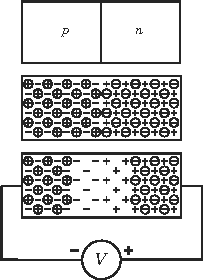
\includegraphics[width=1\linewidth]{Images/LGADs/p-n junction with voltage.png}
    \end{minipage}
    \hfill
    \begin{minipage}[c]{.6\linewidth}
        \caption{\\Top: adjacent regions of \(p\)-doping (left) and \(n\)-doping (right) forming a \(pn\)-junction.\\
        Middle: the circled mobile charges (holes for \(p\)-type and electrons for \(n\)-type) balanced by the charge of atomic cores.\\
        Bottom: when an external (reverse) voltage is applied to the junction, an electric field builds up in the central region, depleting it of free mobile charges \cite{10.1093/acprof:oso/9780198527848.003.0001}.}
        \label{fig:p-n_junction_reverse_bias_voltage}
    \end{minipage}
\end{figure} 

When a charged particle traverses this depletion layer it frees up electron-hole pairs, which move to the electrodes and can be observed as a pulse in the electric potential.
Silicon sensors generally offer several advantages over other type of detectors. The lower energy requirement to produce electron-hole pairs leads to improved energy resolution. Moreover, compared to gas detectors for example, silicon sensors have much higher density, allowing precise measurements in significantly thinner layers. However, this type of device has typically higher manufacturing costs and suffers more considerably from radiation damage.

\subsection{LGADs}

\begin{figure}[h!tbp]
    \begin{minipage}[c]{.45\linewidth}
        \includegraphics[width=1\linewidth]{Images/LGADs/LGADs_schema_of_work.png}
    \end{minipage}
    \hfill
    \begin{minipage}[c]{.4\linewidth}
        \caption{Cutaway view of an LGAD, not to scale. The depletion region makes the majority of the volume of the sensor, and above it, lies the avalanche region. On the left of the picture there is a qualitative plot of the electric field along the vertical axis of the sensor, highlighting the strong electric field in the avalanche region. From \cite{cernTechnicalDesign}.}
        \label{fig:LGADs_schema}
    \end{minipage}
\end{figure} 

A particular type of silicon sensors are Low Gain Avalanche Detectors (LGAD), an illustration is shown in Figure~\ref{fig:LGADs_schema}. The major innovation over standard silicon sensors is an additional \(p\)-type layer below the \(n+\) electrode. This creates a high electric field region which leads to an avalanche effect\footnote[2]{When electrons acquire enough energy they can create new electron-hole pairs ('impact ionization'), which can themselves create new pairs and initialize a multiplication chain that leads to an enhanced signal} of the electrons. 
Charged particles in standard silicon produce roughly 65 e-h pairs per \unit{\micro\meter} of thickness \cite{meroli_energy_loss2011}, equivalent to around \qty{0.52}{\femto\coulomb} for \qty{50}{\micro\meter}. The avalanche effect magnifies the signal around 8-20 times (i.e. a \textit{gain} of 8-20), bringing the collected charge up to \qty{4}{\femto\coulomb}-\qty{10}{\femto\coulomb} \cite{cernTechnicalDesign}. % charged particle in 50 um of silicon produce ~0.52 fC of charge or 3280 e-h pairs

The intrinsic multiplication in LGADs amplifies the signal, improving the signal-to-noise ratio (S/N) and mitigating the signal degradation caused by radiation-induced noise.

The key metrics of the sensors are: time resolution, collected charge and efficiency.

\subsubsection{Time Resolution}

To accomplish a time resolution per track of \(\approx\qty{30}{\pico\second}\) (start) and \(\approx\qty{50}{\pico\second}\) (end), the sensors will require a time resolution per hit of \(\approx\qty{35}{\pico\second}\) (start) \(\approx\qty{70}{\pico\second}\) (end) \cite{CERN-LHCC-2020-007}.

Three major effects determine the time resolution of the sensors: time walk from amplitude variations\footnote{Time walk refers to the variation in signal timing caused by pulses with different amplitudes reaching a fixed threshold at different times.}, electronic noise jitter, and Landau fluctuations from charge deposition non-uniformities. 
\marginpar{\flushleft The plot of time walk effect }

\begin{equation}\label{eq:time_resoltuion_LGADs}
    \sigma^2 = \sigma_{TimeWalk}^2 + \sigma_{Jitter}^2 + \sigma_{Landau}^2  \, .
\end{equation}

 Both time walk and noise jitter depend on the type of readout electronics and depend inversely on the signal slope \(dV/dt\).

\begin{itemize}
    \item \(\sigma_{TimeWalk} = \left[ \frac{V_{th}}{S/t_{rise}}\right]_{RMS}\) where \(V_{th}\) is the threshold voltage, S is the signal (proportional to the gain) and \(t_{rise}\) is the time taken by a signal to go from 10\% to 90\% of the maximum amplitude.
    \item \(\sigma_{Jitter} = \frac{N}{dV/dt} \approx \frac{t_{rise}}{S/N}\) where \(S/N\) is the signal-over-noise ratio.
    \item \(\sigma_{Landau}\) depends on the thickness of the sensor (thinner is better) and the setting of the threshold voltage.
\end{itemize}

It can be noticed that the lowest jitter and time walk errors are achieved with high S/N and small rise time, i.e. thin sensors with high gain. Time walk can also be corrected with reconstruction algorithms, such as constant-fraction-discrimination (CFD), Figure~\ref{fig:constant fraction}.

\begin{figure}[h!btp]
    \centering
    \includegraphics[width=.8\linewidth]{Images/methods/Constant_fraction_1.pdf}
    \captionsetup{width=\captionwidth}
    \caption{Illustration of the \textit{time walk} effect: two pulses with similar shapes, but different amplitudes, can have distinct Time Of Arrivals. Two reconstruction algorithms are compared: Constant Threshold Discriminator (left) and Constant Fraction Discriminator (right). CTD has a fixed threshold value, so the TOA \(t\) is set when the pulse crosses the threshold. For CFD, the time \(t\) corresponds to the moment the pulse reaches a certain fraction of the maximum amplitude, removing the time walk effect.}
    \label{fig:constant fraction}
\end{figure} 


\subsubsection{Radiation damage}

Due to the harsh environment the sensors will be placed in, they will suffer significant damage caused by the extreme flux of highly energetic particles. At the microscopic level, this will cause irregularities in the silicon lattice, altering the bulk and surface properties. At the macroscopic level, there will be an increase in leakage current, a degradation in charge collection efficiency and a change in the effective doping concentration \cite{Moll:1999kv} (as the defects can behave as donors or acceptors). The leakage current can be sufficiently quenched by operating at low temperatures, the charge collection can be improved by applying higher bias voltages. But the last effect has the most detrimental impact on the properties of the sensors, which will deteriorate as the radiation dose increases.


\subsection{Signal generation by charged particles}\label{subsec:charged_particles_distribution}
%%% To find the gain of the sensors we have to first look at the charge deposited on a normal silicon sensor (without gain).
The theoretical probability distribution of the energy loss of heavy particles hitting a thin target (such as the active volume of a silicon sensor) has been solved rigorously by Vavilov in \cite{vavilov_1957}. The namesake distribution is a generalization of the Landau distribution, but its evaluation is more difficult, as it is expressed as an integral over some complicated functions \cite[Eq.(4)]{vavilov_1957}. Fortunately, it can be approximated by more straightforward functions depending on the value of a parameter \(\kappa\) (for a more detailed explanation see \ref{sec:vavilov_vs_landau_distribution}): for \(\kappa\rightarrow0\) the Vavilov distribution can be approximated by a Landau, for \(\kappa>>1\) by a Gaussian.

For the conditions of the tests studied in this thesis \(\kappa\approx \num{1e-8}\), well below the limit, thus the Landau function is a good approximation. It can be expressed by \cite{KOLBIG198497}:

\begin{equation}\label{eq:landau}
    \Phi (\lambda) = \frac{1}{\pi} \int_{0}^{\infty} e^{-\lambda u} u^{-u} \sin (\pi u ) \mathrm{d}u \, .
\end{equation}

Additionally, due to a combination of theoretical corrections \cite{PhysRevA.11.1286} (due to the atomic binding of the electrons) and statistical errors on the measurements, the final distribution of energy deposit follows more accurately the convolution of a Gaussian and a Landau distributions (Figure~\ref{fig:langau_convolution_plot}).

\begin{figure}
    \centering
    \includegraphics[width=.6\linewidth]{Images/LGADs/Landau_Gauss_convolution.png}
    \captionsetup{width=\captionwidth}
    \caption{Plot of Landau function (in blue) and the Landau x Gaussian convolution (in red), with equal Landau parameters and arbitrary units, both normalized to 1.}
    \label{fig:langau_convolution_plot}
\end{figure}



\chapter{Test Beam setup}\label{chap:testbeam_setup}

%%% motivate testbeam
A typical way to test the performance of sensors for High-Energy Physics applications is with test beams: the Devices Under Test (DUTs) are put through a focused flux of high energy particles and their response is read out and analyzed. %%% aka testbeam

The HGTD collaboration has run many test beam campaigns, mainly at CERN and at DESY (Deutsches Elektronen-Synchrotron). The focus of this analysis is the test beam campaign of May 2023, conducted at CERN using a beam of \qty{120}{\giga\electronvolt} pions, provided by SPS.

\begin{figure}[h!tbp]
    \centering
    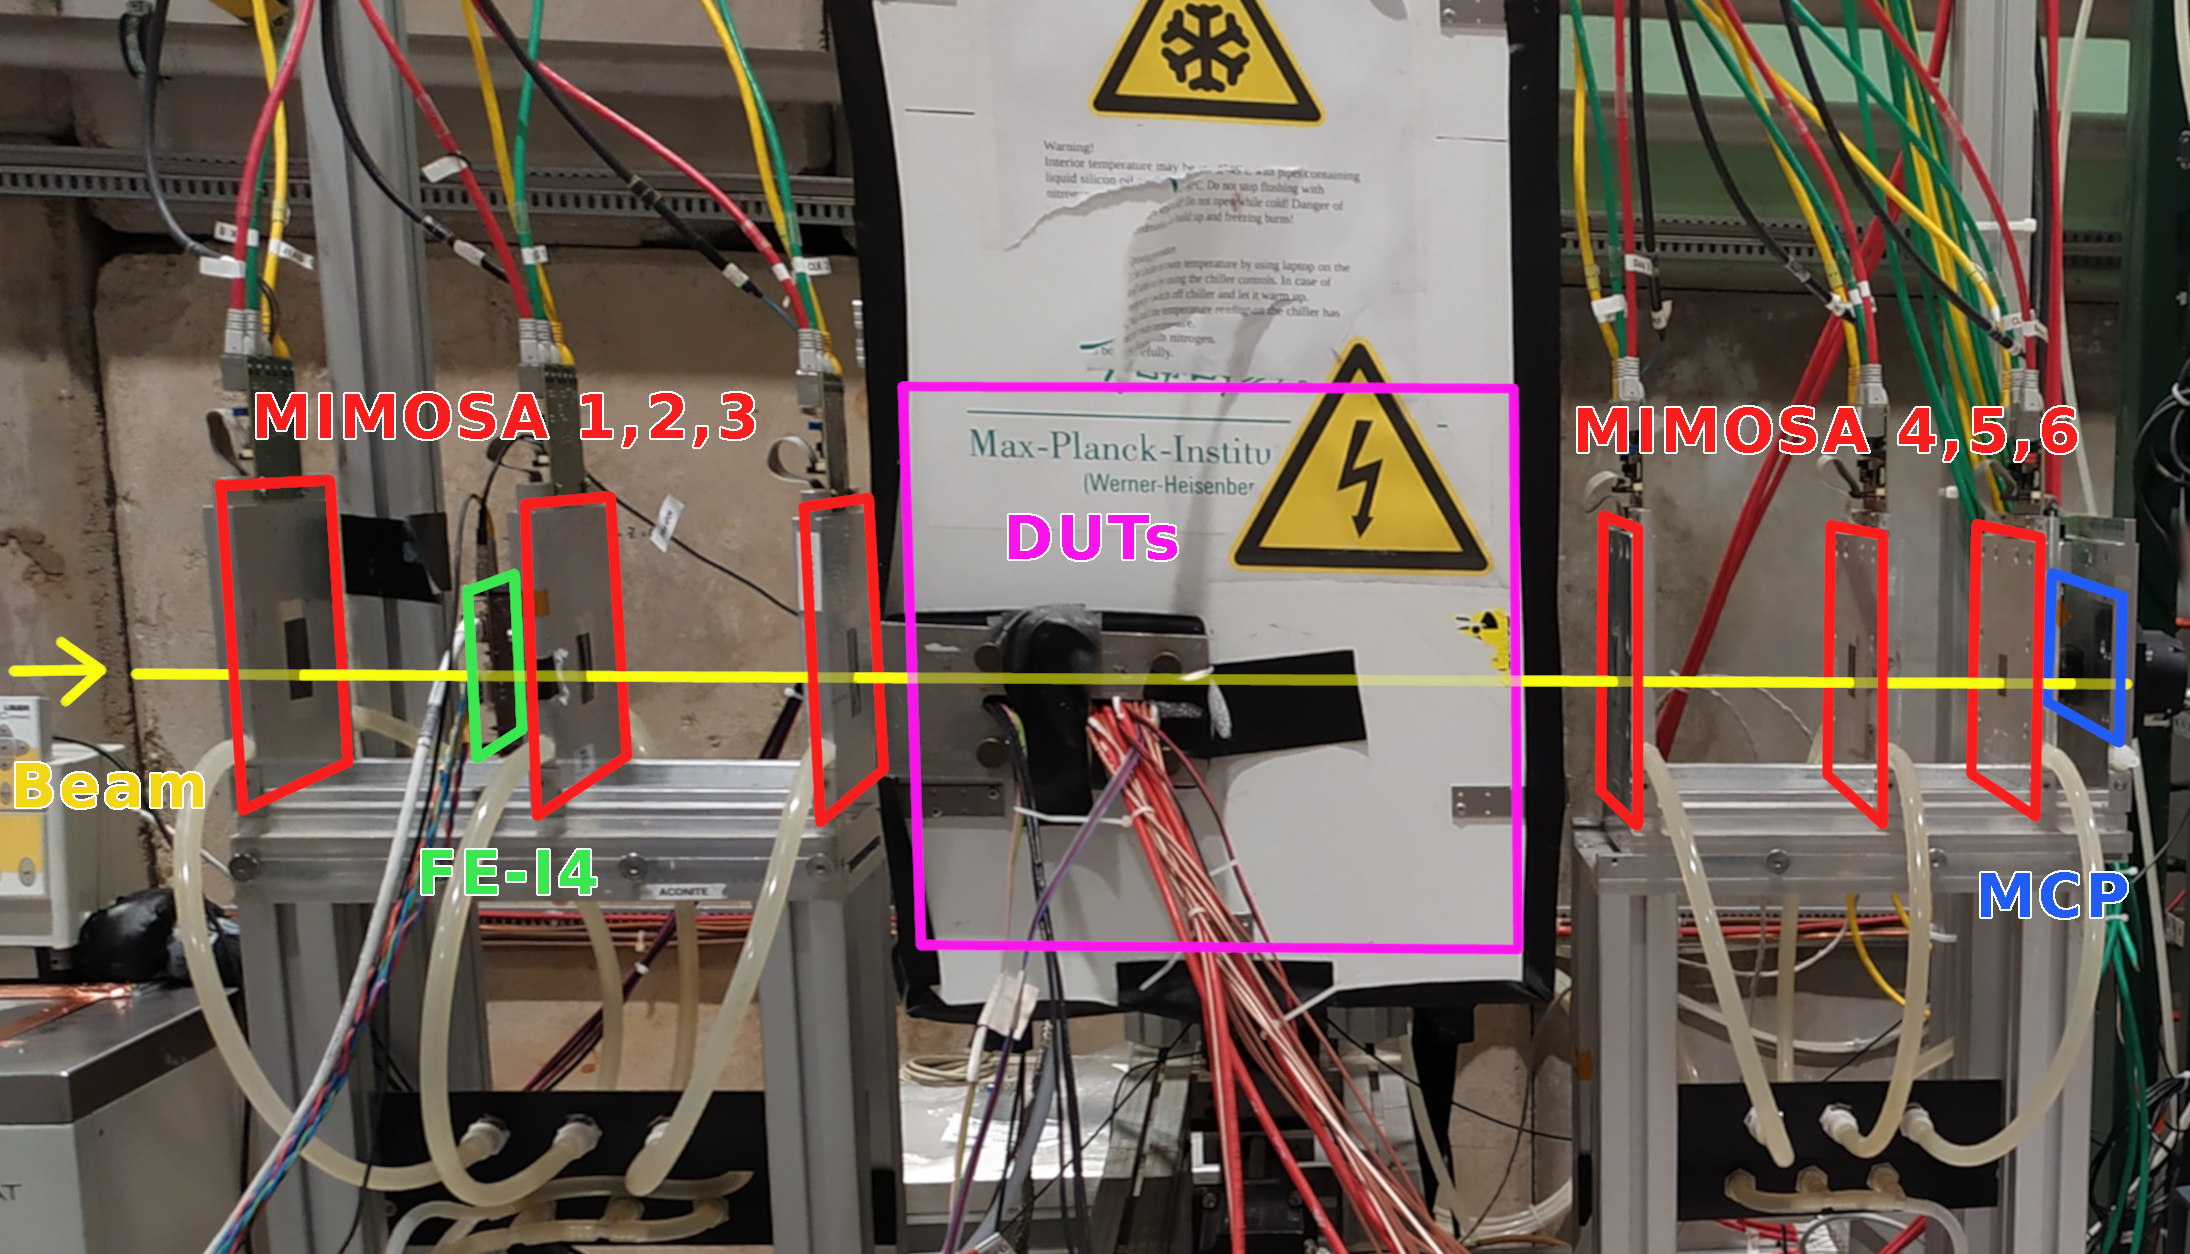
\includegraphics[width=.95\linewidth]{Images/TestBeam_setup/TestBeam_setup_redrawn.png}
    \captionsetup{width=\captionwidth}
    \caption{The main components of the test beam setup: the EUDET-type beam telescope with six MIMOSA planes, the FE-I4, the MCP and the cooling box containing the DUTs}
    \label{fig:testbeam_setup}
\end{figure}

The experimental setup of this campaign included:
\begin{itemize}
    \item FE-i4~\cite{Obermann:2014goa}: a hybrid pixel detector that provided a user-defined Region Of Interest (ROI), creating a HitOR\footnote{A binary signal generated when at least one pixel registers a hit} signal. %to avoid noisy pixels.
    \item Trigger Logic Unit (TLU): provided a trigger\footnote{A trigger is a signal that initiates data readout when a particle is detected}, combining the signals from a scintillator and the FE-i4. %% describe trigger??
    \item EUDET-type beam telescope equipped with 6 MIMOSA planes~\cite{Jansen:2016bkd}: used for precise spatial measurements of the particles in the beam, enabling track reconstruction.
    \item MicroChannel Plate detector (MCP)~\cite{LADISLASWIZA1979587}: measured the time of the moving particles, used as reference for the time resolution.
    \item Cooling box: contained the various DUTs, maintaining them at \qty{-30}{\degreeCelsius}.
    \item 2 oscilloscopes: acquired the data from the MCP and the DUTs. %%% I put later the channels
\end{itemize}

%%% maybe this should just be later

% description of components:
% • Trigger logic unit for particle passing
% • FEi4 to select a region of interest
% • Mimosa planes for tracking (X and Y position data)
% • MCP for time reference 
% • Cooling box containint the DUTs, (can be tilted with respect to the beam direction)
% • 120 GeV beam of pion

\section{TLU and FEi4}

The Trigger Logic Unit provided a trigger whenever a particle was detected. This trigger in turn instructed various components (in this case the oscilloscopes, the MIMOSA planes) to initiate data acquisition. More specifically the TLU took input from a scintillator and the FE-i4 to create a trigger.

The FE-i4 (Front-End-Iteration 4)~\cite{Obermann:2014goa} is a pixel readout chip with a planar silicon sensor bump bonded to it. It has a configurable sensitive area of up to \(\num{16.8} \times \qty{20}{\milli\meter^2}\) made up of 80 columns (\qty{250}{\micro\meter} pitch) and 336 rows (\qty{50}{\micro\meter}). 

Selecting a specific ROI allowed to exclude the areas outside the DUTs surface and to reduce sources of noise (e.g. noisy pixels of MIMOSA planes). %%% maybe the next part is just a repetition of what I say later
%It should be noted that in some occasions, due to erroneous ROI selection or due to small positional shifts caused by temperature fluctuations, the DUTs fell outside said ROI and the analysis was negatively impacted. (Example in Appendix, later)

\section{EUDET-type beam telescope}
A EUDET-type beam telescope~\cite{Jansen:2016bkd} equipped with a total of 6 Minimum Ionizing MOS Active Pixel Sensor planes~\cite{Hu-Guo:2010lrq} provided precise spatial measurements of particle trajectories. Each plane consists of 576 rows and 1152 columns of pixels, each sized \(\qty{18.4}{\micro\meter} \times \qty{18.4}{\micro\meter}\), covering an active area of around \(\num{21.2} \times \qty{10.6}{\micro\meter^2}\). Three of the planes were located before the DUTs, in the direction of the beam, and three were located after. The hits provided by the planes enabled the reconstruction of the tracks of the particles in the beam.

\section{MCP}\label{sec:MCP_description}
The microchannel plate (MCP) detector~\cite{LADISLASWIZA1979587} consists of a single block of resistive material with numerous evenly spaced small tubes (microchannels) connecting one face to the other. The main working principle is similar to that of an electron multiplier. When a voltage is applied between the two sides a potential gradient is established along the channels. Whenever a charged particle hits the inner wall of the tubes multiple secondary electrons are emitted, these electrons then are accelerated and hit the opposite wall in the channel, causing the emission of further secondary electrons. As a result, an exponentially increasing number of electrons can be extracted from the output. This detector can provide very fast response time and, for this reason, it was used as a reference for the time resolution of the other devices.


\begin{figure}
\begin{minipage}[c]{.45\linewidth}
    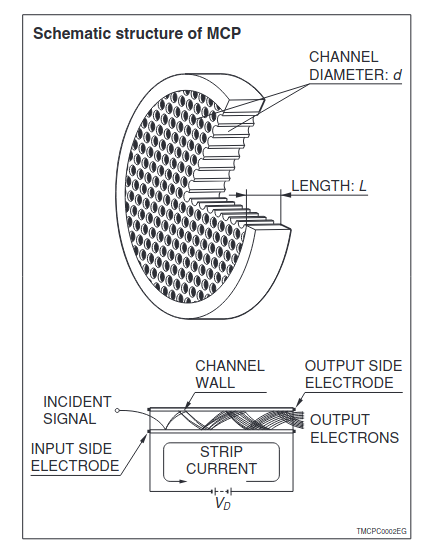
\includegraphics[width=1\linewidth]{Images/TestBeam_setup/MCP diagram HAMAMATSU.png}
\end{minipage}
\hfill
\begin{minipage}[c]{.5\linewidth}
    \caption{
    Schematics of an MCP.\\ 
    Top: structure of the detector with a cross-sectional view of the channels, highlighting the diameter \(d\) and the length \(L\) of the micro-channels. Standard MCPs are fabricated with a diameter of \(10\)s \unit{\micro\meter} and a ratio \(\alpha\) (\(\alpha = L / d\)) 40 to 60.\\
    Bottom: when a voltage (\(V_D\)) is applied, the channel walls behave as continuous electron multiplier: when a target object (electron, ion or photon) hits the inner walls, electrons are released in a parabolic trajectory, and they start a chain reaction which produces a signal amplified by \(10^4-10^7\) times. From~\cite{MCP_figure}.}
\end{minipage}
\label{fig:MCP_diagrame}
\end{figure}


\subsection{Time resolution of the MCP}
The time resolution of the MCP was first calculated by comparing the time difference of two independent sensors (CNM-W4 and CNM-W5, described in Section~\ref{sec:the_sensors}) and the MCP. In this way, it was possible to build a system of three equations of the time differences.

\begin{equation}\label{eq:time_res_system_eqs}
    \begin{cases}
        t_{1-2} = t_1 - t_2  \\
        t_{1-MCP} = t_1 - t_{MCP} \\
        t_{2-MCP} = t_2 - t_{MCP} \, .
    \end{cases}
\end{equation}

The time distributions (left sides of the equations) were fitted with a Gaussian function, each with a width \(\sigma_{ij} = \sigma_i \oplus \sigma_j\), where \(i\) and \(j\) are two of the devices in Equation~\ref{eq:time_res_system_eqs} (i.e. MCP, CNM-W4 and CNM-W5). Assuming that the devices were all independent, their time resolutions would also be independent. This gave a system of three equations with three unknowns, which could be solved analytically to find each individual time resolution: \(\sigma_1\), \(\sigma_2\), \(\sigma_{MCP}\).

This procedure was repeated for all available runs, and the results computed this way are shown in Table \ref{tab:MCP_time_resolution}.
\begin{table}[h!tbp]
    \begin{center}
        \captionsetup{width=\captionwidth}
        \caption{Time resolution values of the MCP. The uncertainty is the standard deviation of all the computed runs.}
        \label{tab:MCP_time_resolution}
        \begin{tabular}{ | c | c | c | c | }
            \hline
            Voltage [\(\si{V}\)] & 2500 & 2600 & 2800 \\ 
            \hline 
            Time resolution [\(\si{ps}\)] & 36.52 & 16.48 & 3.73 \\  
            Uncertainty [\(\si{ps}\)] & \(\pm\)0.81 & \(\pm\)0.57 & \(\pm\)1.33 \\
            \hline
        \end{tabular}
    \end{center}
\end{table}


\section{Oscilloscopes}
The signal generated by the DUT was recorded by two four-channel oscilloscopes: channel 1 (denoted as Ch1) of both oscilloscopes was connected to the MCP (whose signal was put through a splitter and sent to both oscilloscopes). Therefore, up to 6 channels were available in each batch to be attached to the DUTs.
The waveforms recorded by the oscilloscopes were then processed with the PyAna software~\cite{atlas_hgtd_pyana_2025}. 
%  \marginpar{\flushleft I explain this later in the methods}


\section{The sensors}\label{sec:the_sensors}
A variety of LGADs were tested: with different manufacturers, different designs and different fluence\footnote{Radiant exposure, here measured in neutron-equivalent over square centimeters}. They were divided into three main categories:
\begin{itemize}
    \item USTC: from the University of Science and Technology of China.
    \item IHEP: from the Institute of High Energy Physics, China.
    \item CNM: from the Centro Nacional de Microelectr\'onica, Barcelona, Spain.
\end{itemize}

The first two designs have both been manufactured by the IME (Institute of Microelectronics) of the Chinese Academy of Sciences. The two unirradiated CNM sensors (labeled CNM-W4 and CNM-W5) were used to measure the time resolution of another device, the MCP (Section~\ref{sec:MCP_description}), which was used as a time reference for the time measurements of all the other LGADs. 

Two other devices from CNM were irradiated at \qty{1.5e15}{\neutroneq} and \qty{2.5e15}{\neutroneq}. Two versions (v2 and v3) of the IME-IHEP sensors were available, both had a carbon implantation, which has the purpose of increasing the radiation hardness of the LGAD. The sensors were either a single pad or an array (2\(\times\)2 or 1\(\times\)3) of pads, and they were irradiated at fluences ranging from \(0\) to \qty{2.5e15}{\neutroneq}. Two USTC devices, also with carbon enrichment (version 2.1), were tested at zero and low fluence. 

Notably, the data from the irradiated USTC sensor was not available. Moreover, one pad of IMEv3-W12-2x2-1.5E15 was removed from the analysis due a possible wrong labeling (see in Appendix~\ref{sec:mislabeled_sensor}).

The sensors were then installed onto readout boards. In the case of multi-pads sensors, some number of pads were each connected to one channel of the board, so that they could be measured individually.

Table \ref{tab:devices_tested} provides the list of the devices that were characterized.

%%% for more detailed descriptions see Table in \nameref{chap:appendix}.
%%% TODO: maybe more complete table in appendix? with devices id

\begin{table}[h!tbp]  
    \centering
    \captionsetup{width=\captionwidth}
    \caption{List of the tested devices.}
    \label{tab:devices_tested}

    % \makebox[1\textwidth][c]{
    \begin{tabular}{|l|l|l|l|l|l|}
    \hline %%% I NEED TO TRY TO USE TABULAR INSTEAD OF SHORTSTACK
        \textbf{Device name} & \textbf{Vendor} & \begin{tabular}{@{}l@{}}\textbf{Pads,} \\ \textbf{used channels}\end{tabular} & \begin{tabular}{@{}l@{}}\textbf{Fluence} \\ \([n_{eq}/\si{cm^2}]\) \end{tabular} & \begin{tabular}{@{}l@{}} \textbf{Radiation} \\ \textbf{type} \footnotemark \end{tabular}& \textbf{Notes} \\
        \hline
        CNM-W4  & CNM & single & 0 & - & reference \\ 
        CNM-W5  & CNM & single & 0 & - & reference \\ 
        CNM-W5-1.5E15  & CNM & single & \(\num{1.50E+15}\) & neutron & - \\ 
        CNM-W3-2.5E15  & CNM & single & \(\num{2.50E+15}\) & neutron & - \\ 
        USTC2.1-W17 & USTC & 2\(\times\)2, 2 channels  & 0 & - & - \\ 
        USTC2.1-W17-2E14 & USTC & 2\(\times\)2, 1 channel & 0 & - & not available\\ 
        IMEv3-W12-2x2  & IHEP & 2\(\times\)2, 2 channels  & 0 & - & \\ 
        IMEv3-W12-1x3  & IHEP & 1\(\times\)3, 2 channels  & 0 & -  &\\ 
        IMEv3-W12-2x2-1.5E15 & IHEP & 2\(\times\)2, 3 channels  & \(\num{1.50E+15}\) & neutron & only two channels \\ 
        IMEv2-W7-1E14  & IHEP & single & \(\num{1.00E+14}\) & proton & -\\ 
        IMEv2-W7-6.5E14  & IHEP & single & \(\num{6.50E+14}\) & proton  & - \\ 
        IMEv3-W16-8E14  & IHEP & single & \(\num{8.00E+14}\) & proton & - \\
        IMEv3-W16-1x3-1.5E15  & IHEP & 1\(\times\)3, 1 channel  & \(\num{1.50E+15}\) & neutron & no usable batches \\ 
        IMEv3-W16-2.5E15  & IHEP & single & \(\num{2.50E+15}\) & neutron  & - \\ 
        \hline
    \end{tabular}
\end{table}

\footnotetext{\label{footnote:radiation_type} As protons and neutrons interact differently with the atoms of the silicon lattice, they can introduce distinct defect structures. In addition, the enrichment of various impurities may lead to further differences in the type of damage \cite{Ruzin:1999ck}.}

%%% NOT UPDATED ANYMORE, LOOK AT THE EXCEL FILE, I MIGHT DELETE THIS LATER
%%% I have to reorganize these and associate them with the more accurate descriptions
% device name:        vendor:        sensor ID:            fluence:    irradiation type:    type:        board name:    channels:
% CNM-W4              CNM          CNM-R15973-W4-D168      unirradiated      -             single pad     JSI-B12      1
% CNM-W5              CNM          CNM-R15973-W5-D138      unirradiated      -             single pad     JSI-B14      1
% CNM-W3-2.5E15       CNM          CNM-R15973-W3-D29       $\num{2.5e15}     neutron       single pad     JSI B5       1
% CNM-W5-1.5E15       CNM          CNM-R15973-W5-D29       $\num{1.5e15}     neutron       single pad     JSI PP1      1
% USTC2.1             USTC         USTC2.1-W17-P6-A          0                -             2\(\times\)2           CERN-3       1,2
% USTC2.1 IRRADIATED (MISSING)
% IMEv3-W12-C2         IHEP        IMEv3-W12-C2-2-2          0               -              2\(\times\)2          CERN-1       channels 1,2
% IMEv3-W12-C3         IHEP        IMEv3-W12-C3-1-4 (and 5)  0               -              1x3          CERN-1       channles 3,4  (small GR), bonded
% CERN2-CH0-IMEv3-W12  IHEP        IMEv3-W12-B2-2-9-1       1.5e15           neutron        2\(\times\)2 sensor    CERN-2       channels 1,2,3
% CERN2-CH1-IMEv3-W12  IHEP 
% CERN2-CH2-IMEv3-W12  IHEP 
% CERN2-CH4-IMEv3-W16  IHEP        IMEv3-W16-Q4-D4-1-4      1.5e15           neutron        1x3          CERN-2       channel:  2(?)
% JSI-B6-IMEv2-W7-1E14    IHEP       W7-II-C2-1-7 IMEv2-W7Q2    1e14          proton        single       JSI-B6
% JSI-PP4-IMEv2-W7-6.5E14 IHEP       W7-II-C2-1-7 IMEv2-W7Q2    6.5e14        proton        single       JSI-PP4
% JSI-B7-IMEv3-W16-8E14   IHEP       IHEP-IMEv3-W16_Q4_D3_1-4   8e14          (unsure)        single       JSI-B7
% JSI-B13-IMEv3-W16-2.5E15 IHEP      IHEP-IMEv3-W16_Q4_E3_1-4   2.5e15       (unsure)      single        JSI-B13
                 

\chapter{Analysis}\label{chap:methods}
%%% I need to restructure deeply

The data recorded by the oscilloscopes, in the form of waveforms, was pre-processed using the software PyAna~\cite{atlas_hgtd_pyana_2025}. Another software, PaTrack~\cite{atlas_hgtd_patrack_2025}, used the spacial information from the MIMOSA planes to reconstruct the tracks of the particles. The data was then combined into ROOT files to be further analyed.


Some quality cuts were applied to the data, to remove extra noise. To illustrate the analysis procedure that was followed in this study, a single DUT was picked as an example. All the plots in this chapter (unless otherwise stated) refer to the sensor IMEv3-W12, a 2\(\times\)2 array of LGADs, operated at \qty{-30}{\degreeCelsius} and perpendicular to the beam.

\section{Data pre-processing}

The pre-processing was performed by other collaborators prior to this analysis. The steps of the pre-processing are described below.

\begin{figure}[h!btp]
    \centering
    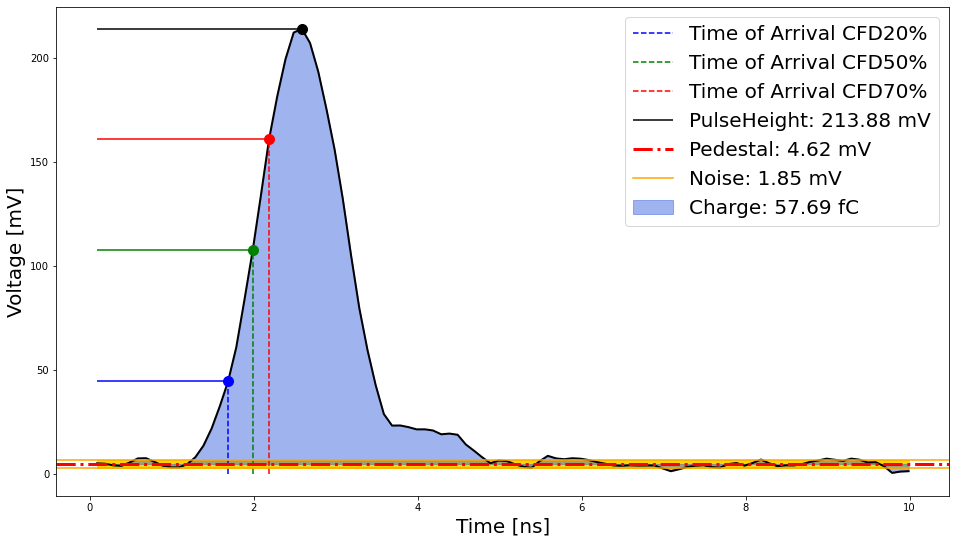
\includegraphics[width=1\linewidth]{Images/methods/Waveform of particle, channel2, with CFD (ns).png}
    \captionsetup{width=\captionwidth}
    \caption{An example of a pulse with its main features highlighted. The pedestal (red dotted line) is the mean of the background signals, the noise (yellow) is its standard deviation, the pulseheight (black) is the maximum amplitude and the charge (light blue) is the area under the pulse. The remaining three dashed lines (blue, green and red) correspond to the TOA associated to three different values of CFD (20\%, 50\% and 70\%, respectively).}
    \label{fig:waveform_features}
\end{figure} 

%PyAna, aka pulse description
Whenever a trigger was detected, the oscilloscopes recorded an event. For each event, at least 2000 samples were collected, spaced every \qty{25}{\pico\second}, an example of one event (a pulse) is shown in Figure~\ref{fig:waveform_features}. This pulse (waveform) was then processed with PyAna.

Firstly, the pedestal and the noise were measured by computing the mean and standard deviation, respectively, using the first 240 samples, where no signal is expected \cite{Allaire:2018bof}. Secondly, the maximum of the pulse was found by a second-degree polynomial fit, in a \qty{400}{\pico\second} window around the sample with the highest amplitude. After subtracting the pedestal, the total charge was computed as the integral of the pulse divided by the transimpedance\footnote{Trasfer impedance, it is the ratio of output voltage to input current in the readout board, expressed in \unit{\ohm}} value of the board the LGAD is mounted on (Equation~\ref{eq:charge_integral}). The integral is computed in a window wide enough to contain the full pulse.

\begin{equation}\label{eq:charge_integral}
    Q = \frac{\int_{t_1}^{t_2} V(t)dt}{R_b} \, .
\end{equation}
Where \(Q\) is the charge, \(V\) is the voltage (as a function of time \(t\)), \(R_b\) is the transimpedance and \(t_2-t_1\) is the integration window.

%%% PaTrack, aka MIMOSA plane
The spacial information was processed with the PaTrack software to create tracks of the particles. Two straight tracklets, an "upstream" and a "downstream" tracklet passing through MIMOSA planes 1,2,3 and 4,5,6, respectively, were reconstructed to best fit the hits on each plane and meet at the longitudinal (z) location of the DUTs, Figure~\ref{fig:mimosa_tracking}. This provided each event with the XY intersection of the track onto the plane of each DUT. 

\begin{figure}[h!btp]
    \centering
    \includegraphics[width=1\linewidth]{Images/methods/MIMOSA tracking scheme.png}
    \captionsetup{width=\captionwidth}
    \caption{Scheme of the reconstructed tracks, made of two tracklets, one upstream and one upstream, as they best fit the hits on the MIMOSA planes before and after the DUTs.}
    \label{fig:mimosa_tracking}
\end{figure} 


To measure the time resolution it is crucial to define the Time of Arrival (TOA), i.e. the time at which the particle hits the sensor and the pulse is recorded. There are several ways to make this choice, including: Constant Threshold Discriminator (CTD), Constant Fraction Discriminator (CFD) and Zero Crossing Detector (ZCD).

\begin{figure}[h!btp]
    \centering
    \includegraphics[width=.8\linewidth]{Images/methods/Constant_fraction_1.pdf}
    \captionsetup{width=\captionwidth}
    \caption{Comparison of Constant Threshold Discriminator (left) and Constant Fraction Discriminator (right), for two pulses with similar shapes but different amplitudes. CTD has a fixed threshold value, the TOA \(t\) is set when the pulse crosses the threshold. For CFD, the time \(t\) corresponds to the moment the pulse reaches a certain fraction of the maximum amplitude. This illustrates the \textit{time walk} effect.}
    \label{fig:constant fraction}
\end{figure} 

In this study we chose to use the Constant Fraction Discriminator. More specifically, for the MCP a value of 50\% CFD was chosen, while for the DUTS a value of 20\% was chosen in all cases except for heavily irradiated sensors, in which 70\% yielded improved results overall.

\FloatBarrier

\section{Quality cuts}\label{sec:qualtiy_cuts}

% To remove the various sources of noise some quality cuts were applied to the data. %; in this section we explain these choices.
To ensure that only physically meaningful events were used in the measurements, it was necessary to apply some quality cuts to the initial data. These cuts were designed to reject events affected by various sources of noise or not meaningful to the analysis. 
%%% TODO: maybe more examples? 

To begin with, we removed events with low signal peak (or high noise). Subsequently, we used the pulse height information to identify the outline of each pad and select only events passing through it. Finally, we established a time window around the peak of the distribution to avoid negative effects caused by the neighbouring pads and the edges of the sensors (outside the gain layer).

\subsection{Noise cut}\label{subsec:noise_cut}
The most straightforward trimming consisted in the exclusion of signals which had a pulseheight less than 3 times greater than the noise:

\begin{equation*}
    P > b + 3\sigma \, .
\end{equation*}

Where \(P\) is the maximum of the pulse (pulseheight), \(b\) is pedestal baseline and \(\sigma\) is the noise. This ensured the exclusion of events that could simply be particularly highly peaked noise. %%% don't know about this sentence

\subsection{Pulse height cut}\label{subsec:pulseHeight_cut}

% I think I want to cut out the title
\begin{figure}[h!tbp]
    \centering
    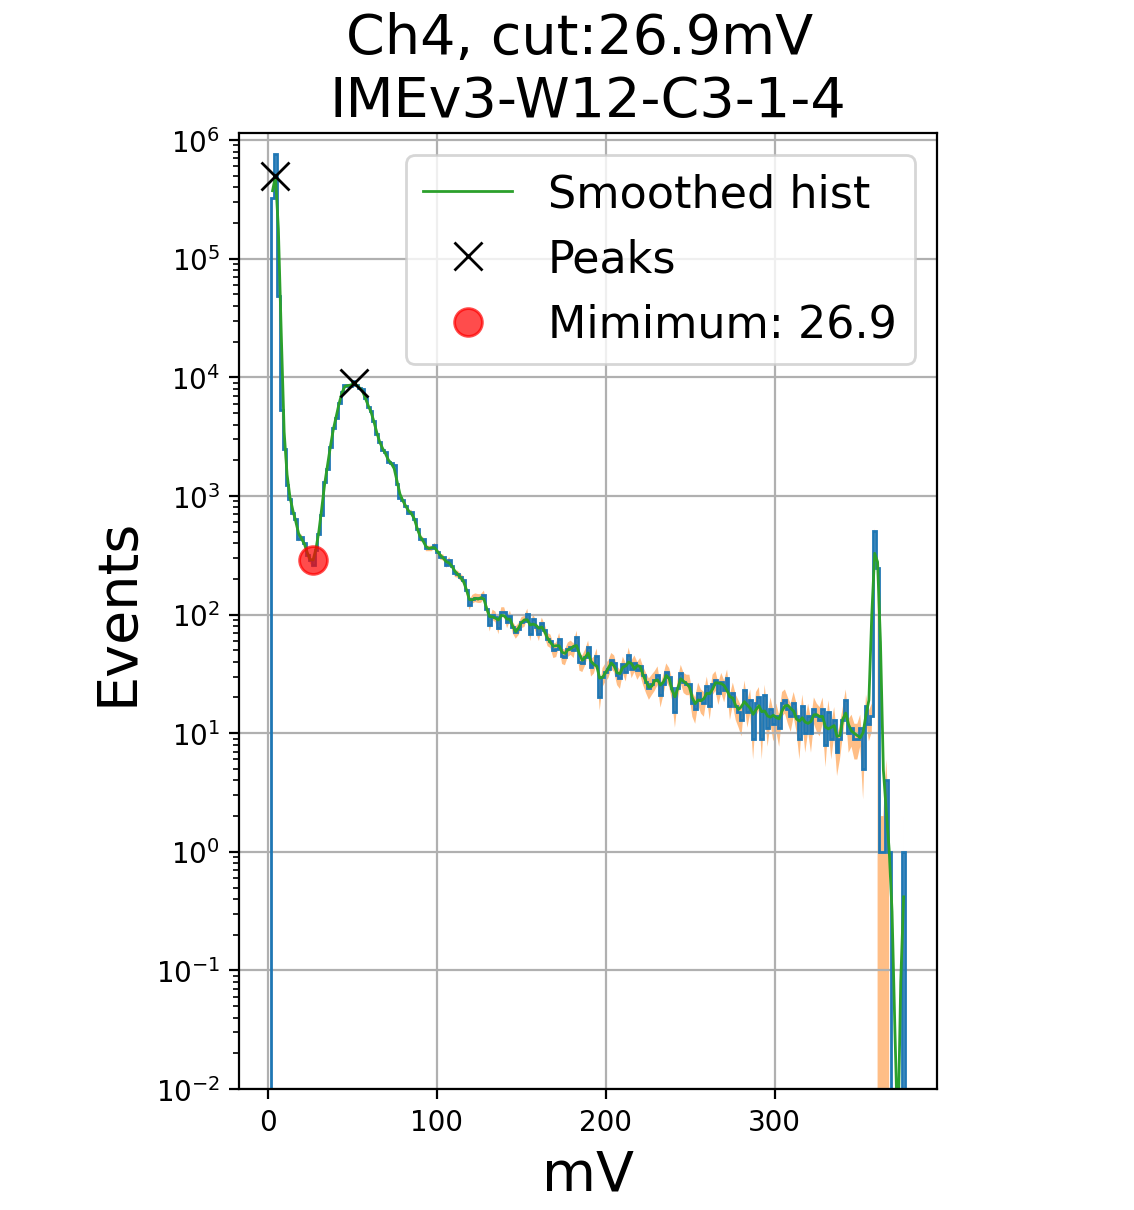
\includegraphics[width=.5\linewidth]{Images/methods/2D_Sensors_401 S1 pulseHeight cut_pulse.png}
    \captionsetup{width=\captionwidth}
    \caption{The pulse height cut was defined by the position of the local minimum between the two main peaks (identified as to noise and signal)}
    \label{fig:pulseHeight_cut}
\end{figure}

By plotting the distribution of pulse height values, we applied a cut to the pulses located below the local minimum in the distribution\footnote{A Kernel Density Estimator was used in order to smooth the distribution before identifying the minimum}, to separate guaranteed signals from potential noise. The goal of this cut was to select only events that were detected by the DUT, and use this information to find the physical outline of the pad.

Using this selection of events, the X and Y coordinates of the tracks were plotted, giving the result shown in Figure~\ref{fig:pulseHeight_cut_highlight}. The outline of the sensor is distinctly shown, making possible the subsequent quality cut: the selection of tracks that passed through the surface of the pad, i.e. a \textit{geometry cut}

\subsection{Geometry cut}\label{sec:geometry_cut}

\begin{figure}[h!tbp]
    \centering
    % \includesvg[width=1\linewidth]{Images/methods/locating_edges_Xtr_batch_401_S1_DUT3}
    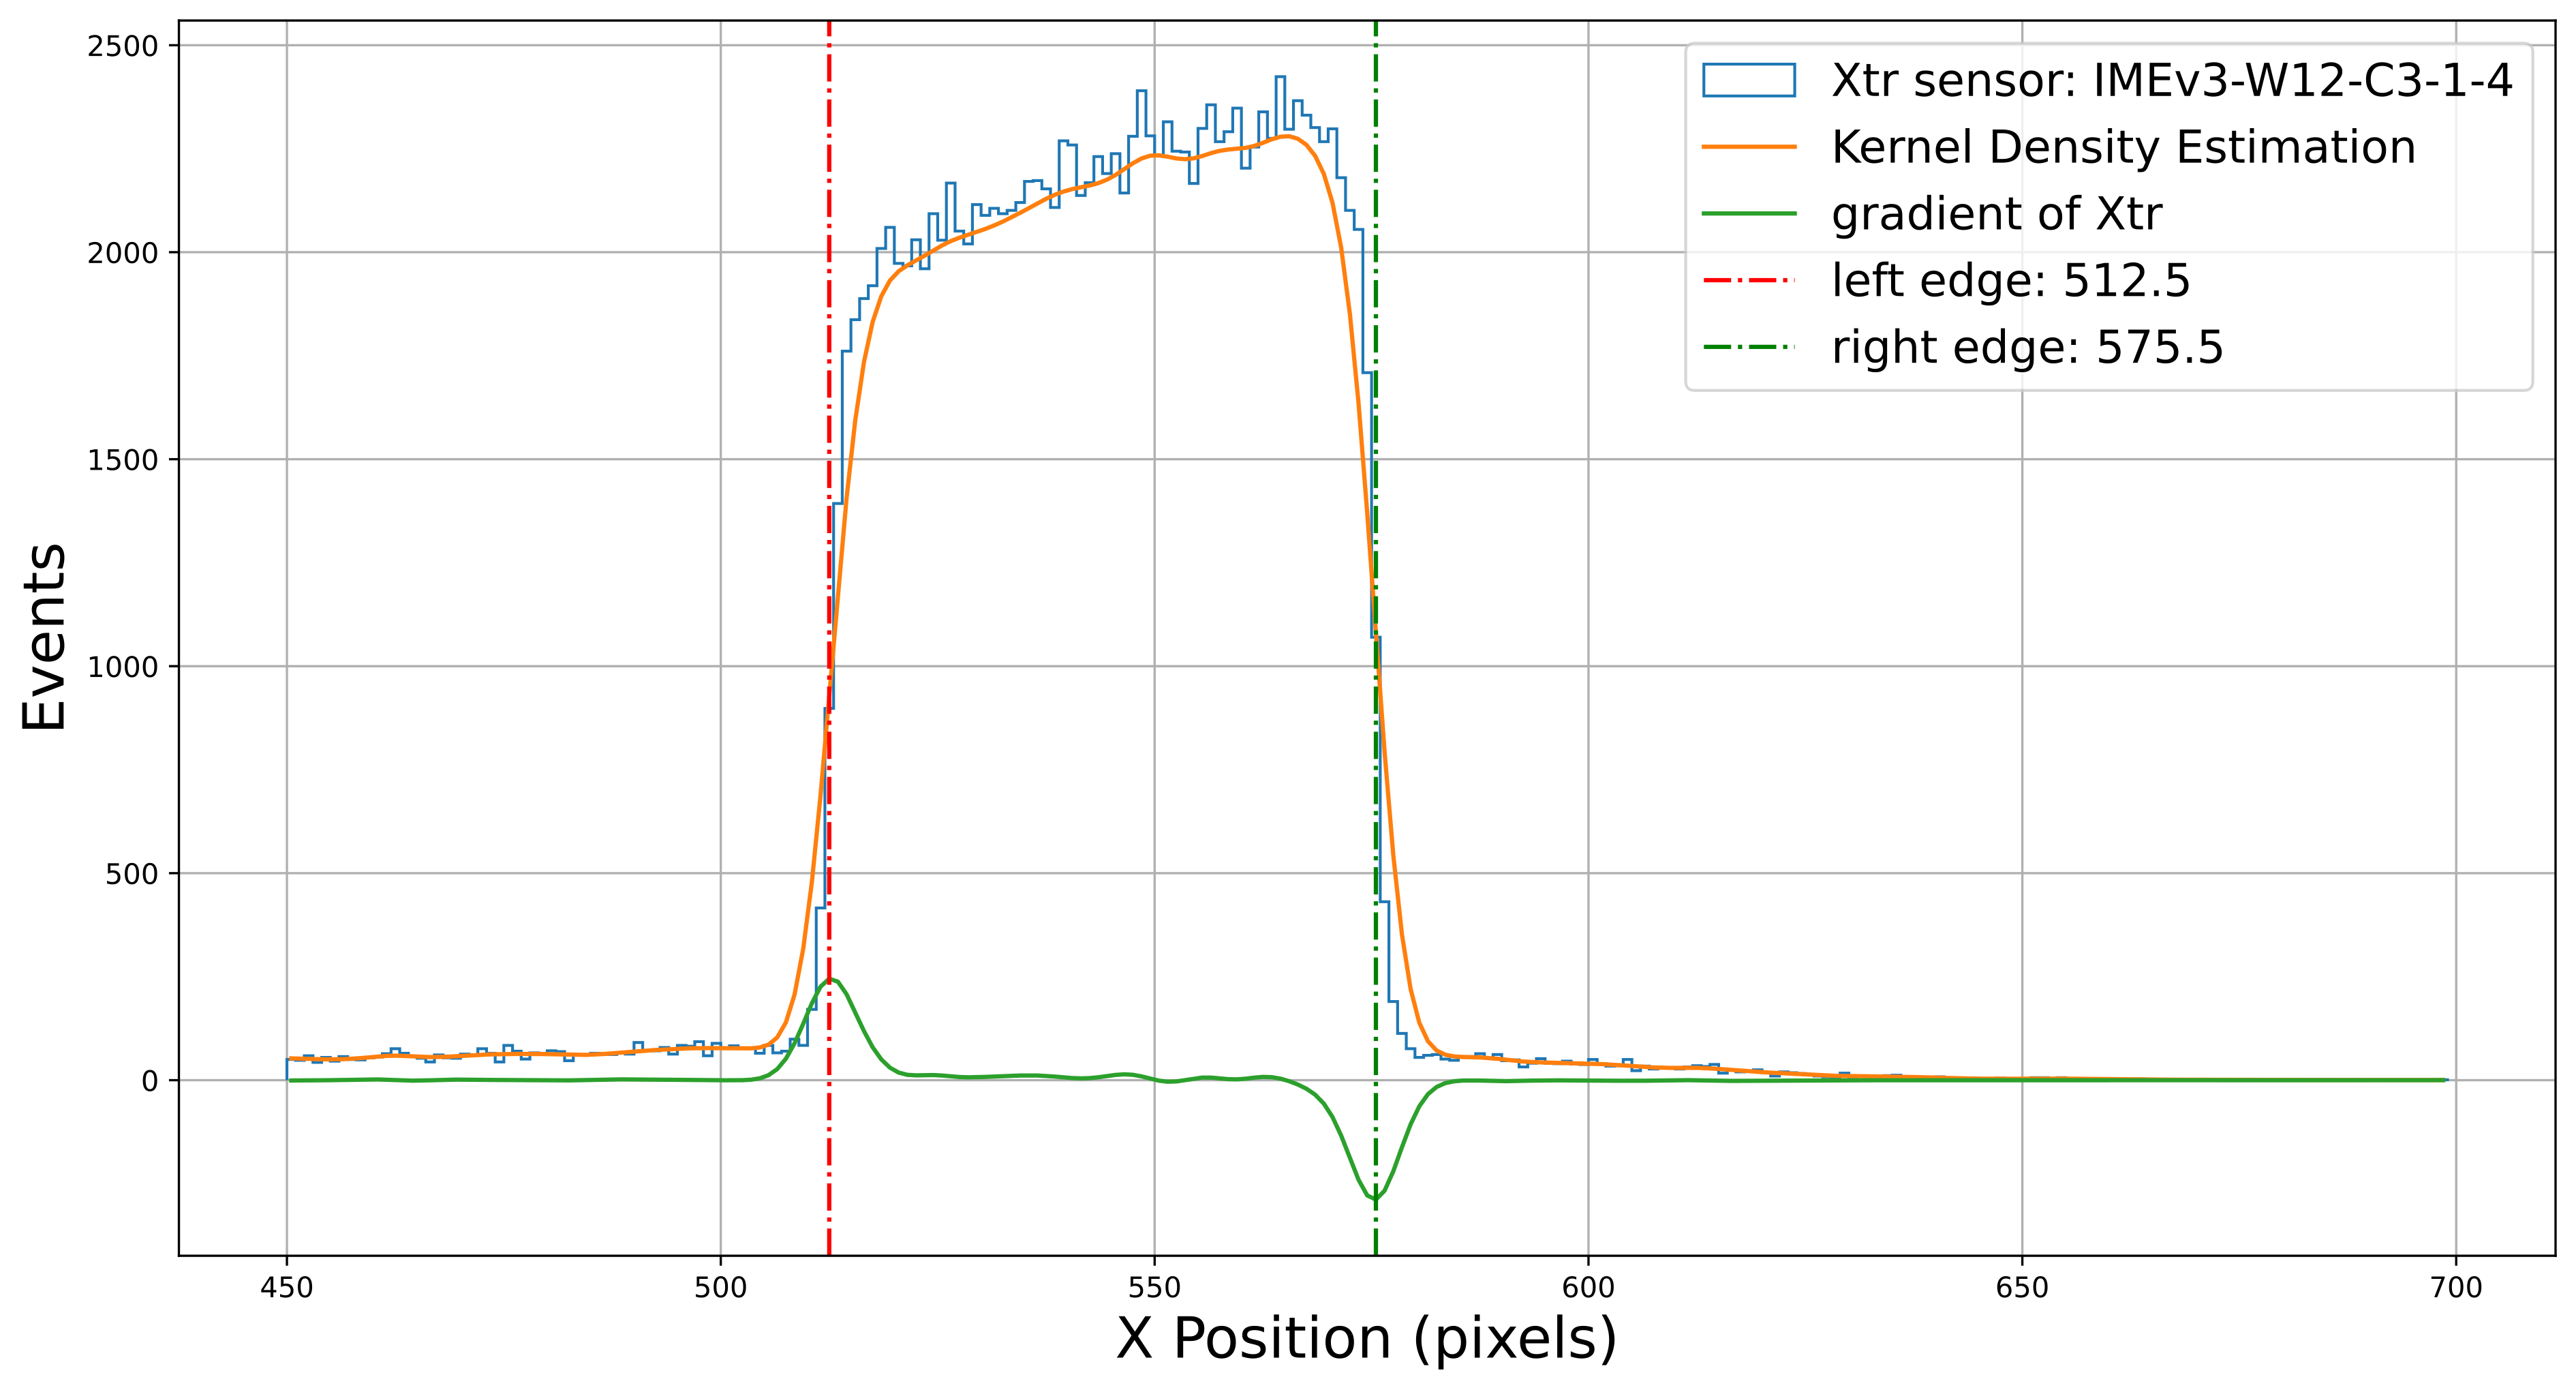
\includegraphics[width=.7\linewidth]{Images/methods/locating_edges_Xtr_batch_401_S1_DUT3.png}
    \captionsetup{width=\captionwidth}
    \caption{Projection of hits on the X axis after the \nameref{subsec:pulseHeight_cut}. By taking its derivative, it was possible to determine the position of the edges of the sensor. The unit is pixels of MIMOSA planes.}
    \label{fig:edges_of_the_sensor}
\end{figure}

Looking at the projections of hits on the X and Y coordinates, it was possible to determine the outline of the pad. The distribution was smoothed\footnote{Using a Kernel Density Estimator, as done previously for the pulse height distribution in Section \ref{subsec:pulseHeight_cut}} and its gradient (derivative) was calculated. This gave rise to two remarkably pronounced peaks shown in Figure~\ref{fig:edges_of_the_sensor}, which could be interpreted as the edges of the pads. By applying this procedure to both the X and Y projections we determined the horizontal and vertical edges, respectively. The final rectangular shape can be seen in Figure~\ref{fig:pulseHeight_cut_highlight}, alongside with the density of hits after applying a \textit{pulseHeight cut}. In few cases the sensors were slightly tilted in the XY plane, giving rise to slightly imprecise outlines, this is shown in Appendix, although it did not have a significant impact on the rest of the analysis.
%%% TODO: example of imprecise outlines

% NOTE: the edges defined like this are smaller than the real size of the pad (which is 1.3x1.3 mm\(^2\)) \cite{Agapopoulou_2022} \marginpar{\flushleft There is an outer guard ring isolating, so maybe the size is correct}

For certain properties that were analysed (such as efficiency and time resolution) it became clear that the rough selection of the contour of the pad was not always sufficient. Thus, an additional \textit{central area cut} was set up. A region of \(0.5\times0.5\si{mm^2}\) in the center of the pad was selected (similarly to what had been done in \cite{Agapopoulou_2022}) in order to avoid undesirable effects originating from the region outside the gain layer of the LGAD. (maybe details about LGADs guard ring and front view?)

\begin{figure}[h!tbp]
    \centering
    \subfloat[The heatmap of the reconstructed tracks without any cuts applied. The large rectangular shape is produced by the region of interest (ROI) selected with the FE-I4.]{
        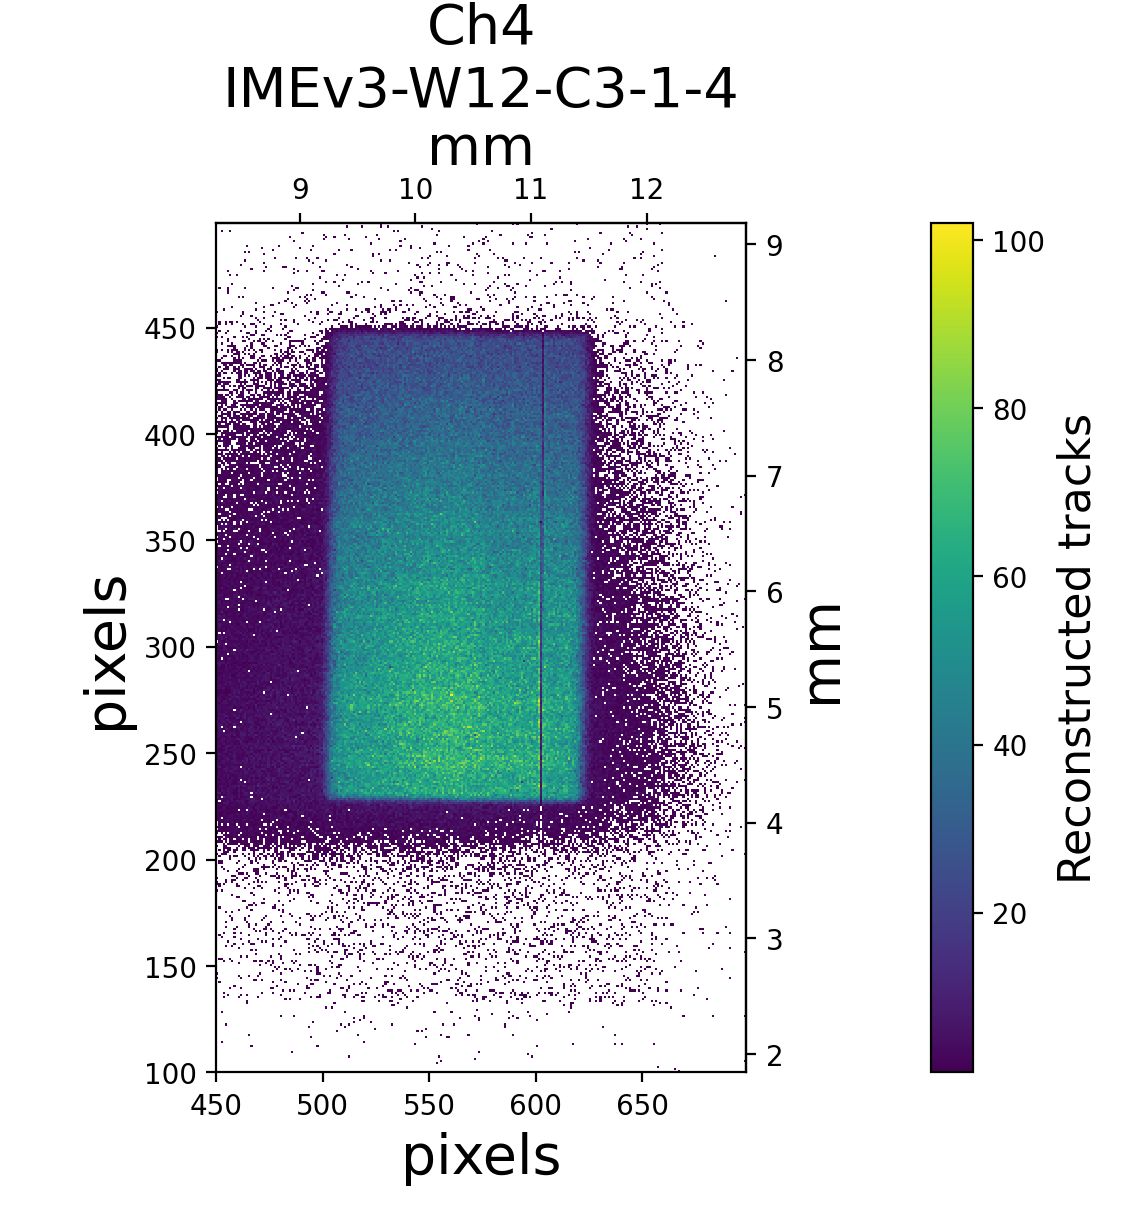
\includegraphics[width=.47\linewidth]{Images/methods/2D_Tracks_401 S1 (no cuts)_DUTs_3.png}
        \label{fig:hits_no_cuts}}
    \hfill
    \subfloat[The smaller rectangle corresponds to the area of the pad (highlighted in red with sides lengths) found by applying a \textit{pulseHeight cut}.]{
        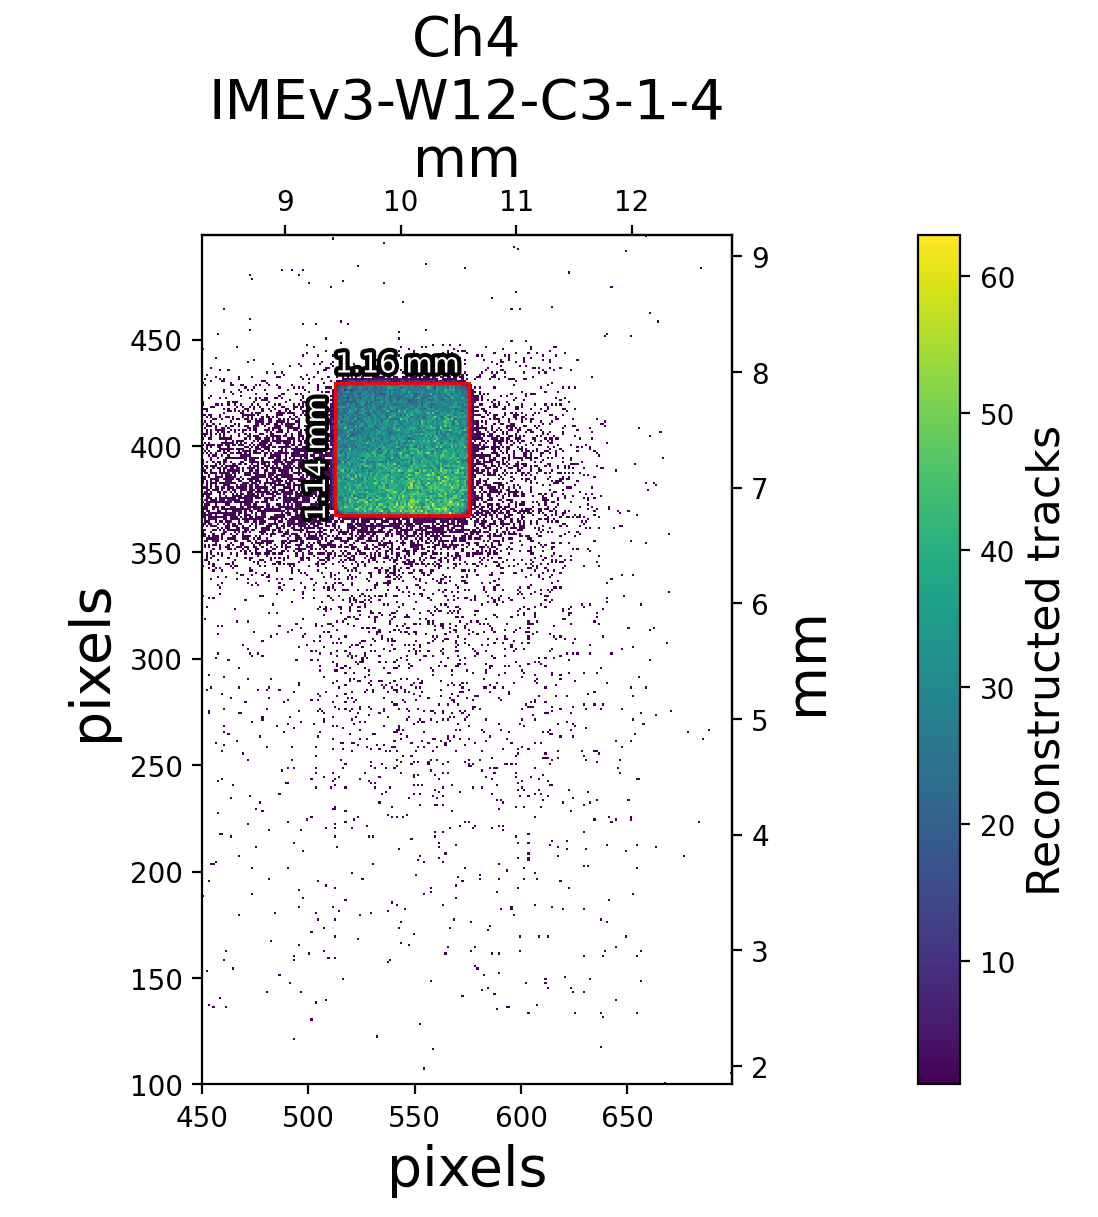
\includegraphics[width=.45\linewidth]{Images/methods/2D_Tracks_401_S1 highlight geometry cut (using pulseHeight).png}
        \label{fig:pulseHeight_cut_highlight}}
    \captionsetup{width=\captionwidth}
    \caption{later}
\end{figure}

\subsection{Time cut}\label{subsec:time_cut}

Additionally, to further clean the data, a cut on the \(\Delta t\) was applied.

Firstly the distribution of \(\Delta t\) (\(t_{DUT}-t_{MCP}\), time of arrival of the DUT - MCP) without any other cut was fit with a Gaussian plus a uniform background (Figure~\ref{fig:time_cut_gauss+bg_fit}):

\begin{figure}[h!tbp]
    \centering
    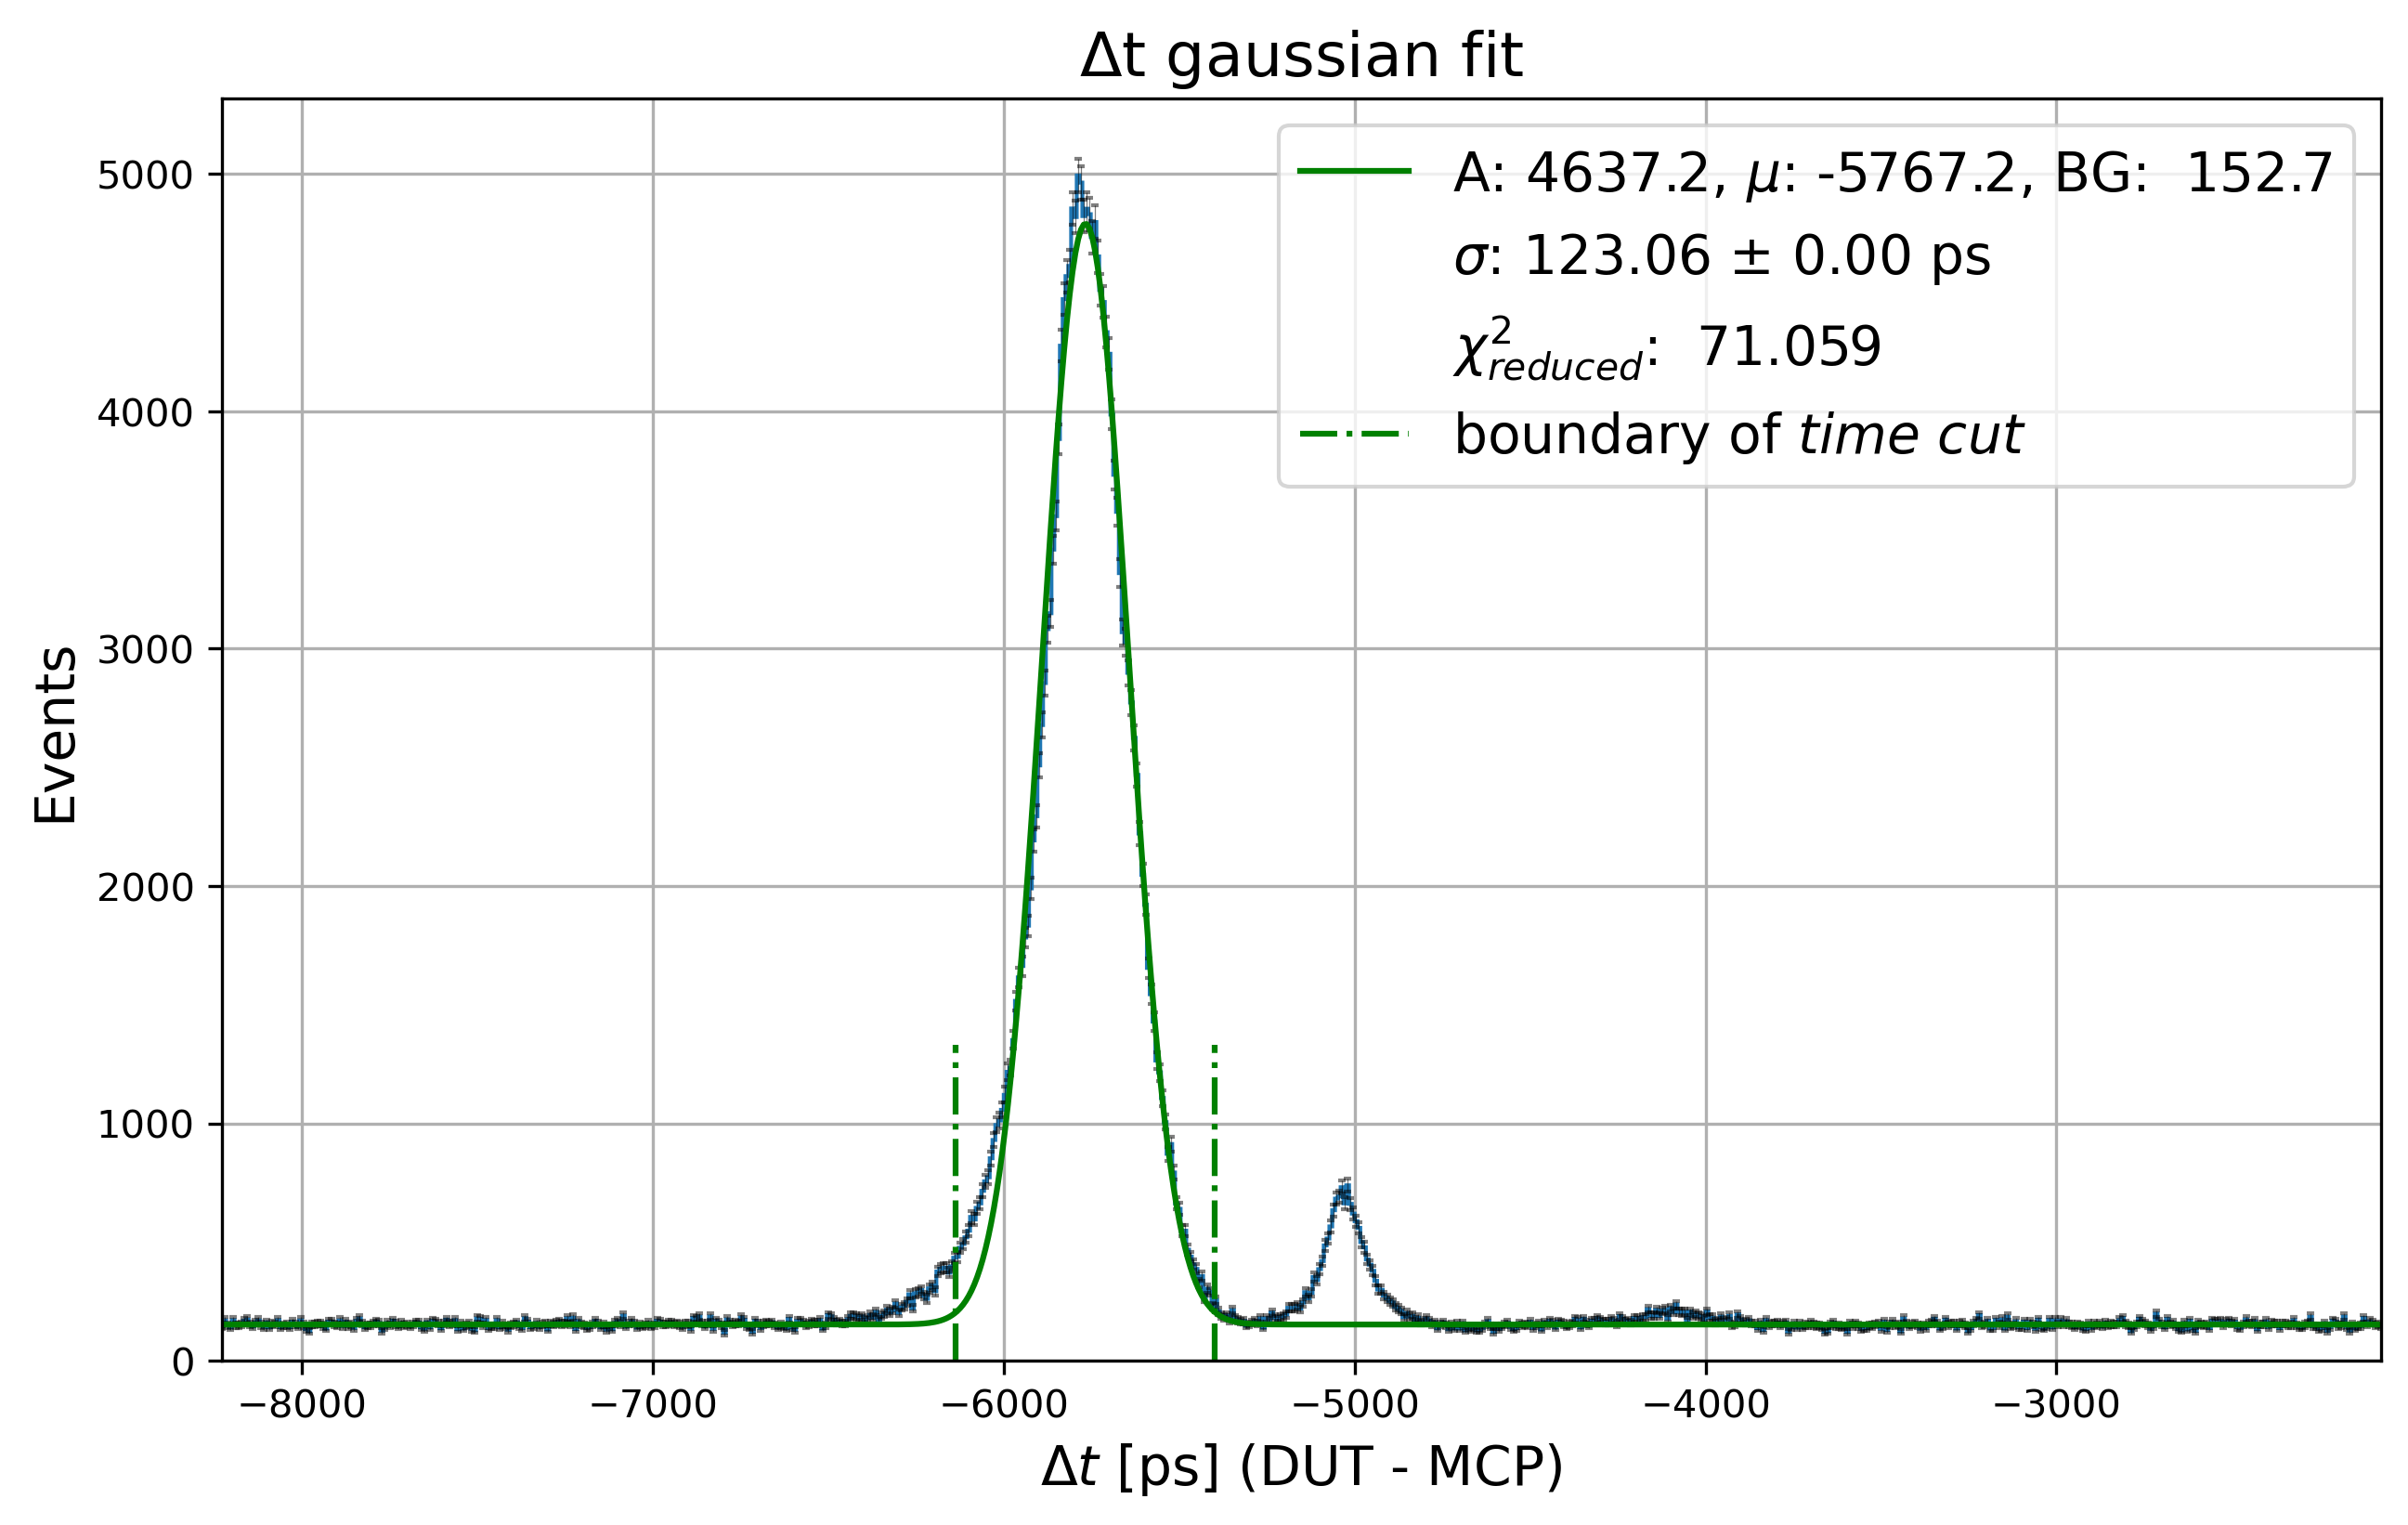
\includegraphics[width=.9\linewidth]{Images/methods/time_difference_603_S2_gauss_fit_no_cuts_DUT2.png}
    \captionsetup{width=\captionwidth}
    \caption{Time difference distribution (\(t_{DUT}-t_{MCP}\)) fit with a Gaussian + uniform background. The vertical dashed lines represent the boundary set as \textit{time cut}. The secondary peak 
     the right (i.e. delayed) is caused by a neighbouring pad, more detailed explanation in Section~\ref{sec:multiple_peaks}.}
    \label{fig:time_cut_gauss+bg_fit}
\end{figure}

\begin{equation*}
    f(x,A,\mu,\sigma,BG) = A \cdot e^{-\frac{1}{2}\left(\frac{x-\mu}{\sigma} \right)^2} + BG  \, .
\end{equation*}

\(A:\) Amplitude (n° of events);\quad \(\mu:\) Mean of the gaussian;\quad \(\sigma:\) Standard deviation;\quad \(BG:\) Uniform BackGround.

Ultimately, a \textit{time cut} was defined as all the events lying inside an interval of a number \(n\) of standard deviations \(\sigma\):

\begin{equation}
    (\mu-n\sigma;\mu+n\sigma) \, .
\end{equation}

Given that roughly 99.7\% of all values of a normal distribution lie within 3 standard deviations, \(n=3\) was deemed an adequate choice.

This cut proved to be especially useful in calculating the total efficiency of each pad and in fitting the charge distribution.

Some peculiarities became apparent, namely the second peak shifted to the right of the main one (meaning delayed compared to the latter) and some discrepancy with the expected Gaussian distribution around the left tail. These effects were further investigated and will be explained later in Sections \ref{sec:multiple_peaks} and \ref{sec:deviations_from_gaussian}.

\subsubsection{Heavily radiated sensor case}\label{subsec:geometry_cut_w/pulse_cut}

In some cases, typically for heavily radiated sensors, the noise in the pulse height distribution was too large (Figure~\ref{fig:pulseHeight_cut_failed}) to allow a \textit{pulseHeight cut} as in \ref{subsec:pulseHeight_cut}. This happened due to the pulse height decreasing and the noise peaks rising, so the separation between the two became less marked. In these situations it was possible to apply a \textit{time cut} instead and still get a satisfactory contour of the pad. The results between the two methods were very similar (Figure~\ref{fig:geometry_cut_comparison} in \nameref{chap:appendix}) so this seemed a good alternative.

\begin{figure}[ht]
    \centering
    \subfloat[Pulse height distribution, without a clear boundary between noise and signal.]{
        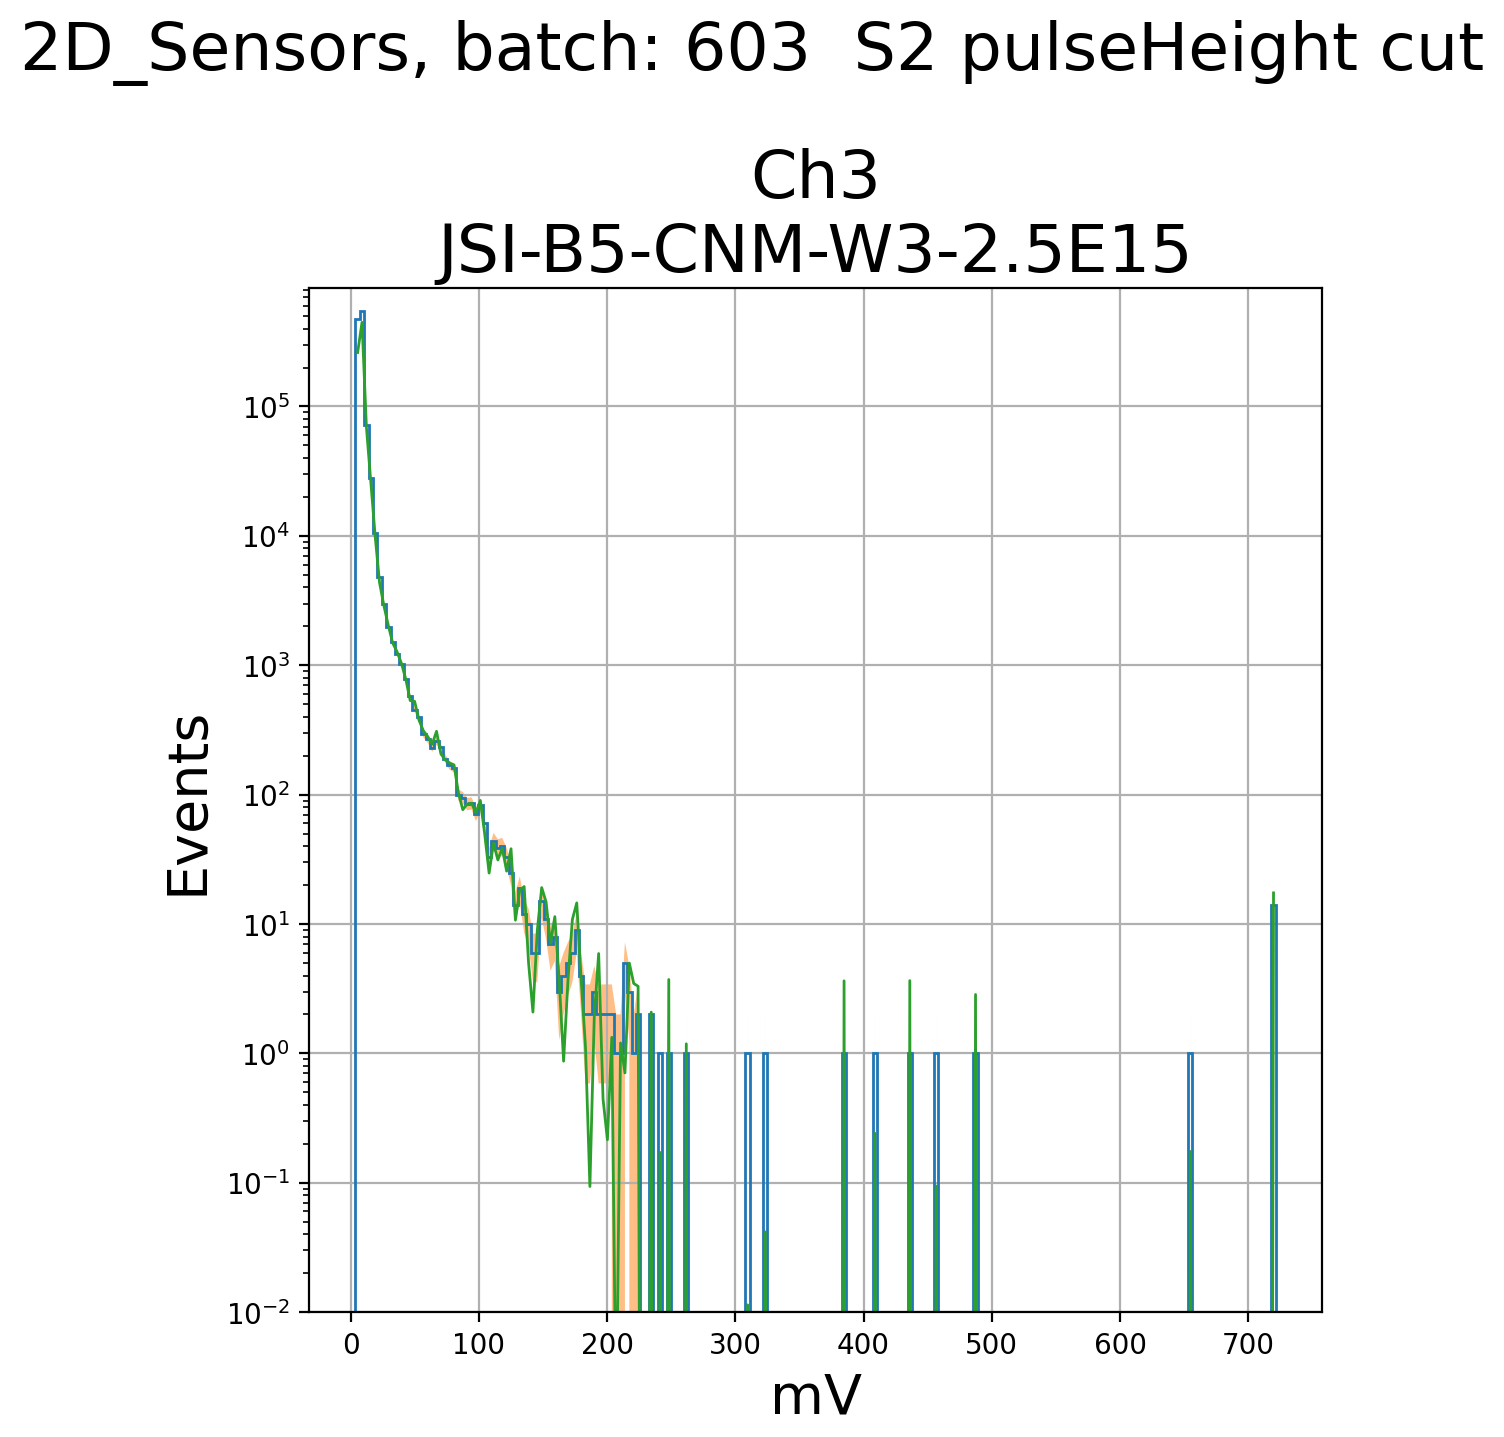
\includegraphics[width=.5\linewidth]{Images/methods/2D_Sensors_603 S2 pulseHeight cut_only_pulse.png}
        \label{fig:pulseHeight_cut_failed}}
    \hfill
    \centering
    \subfloat[Contour of the pad, highlighted in red, found by applying a time cut to the data. The irregular shape of the pad is caused by the ROI selected by the FEi4.]{
        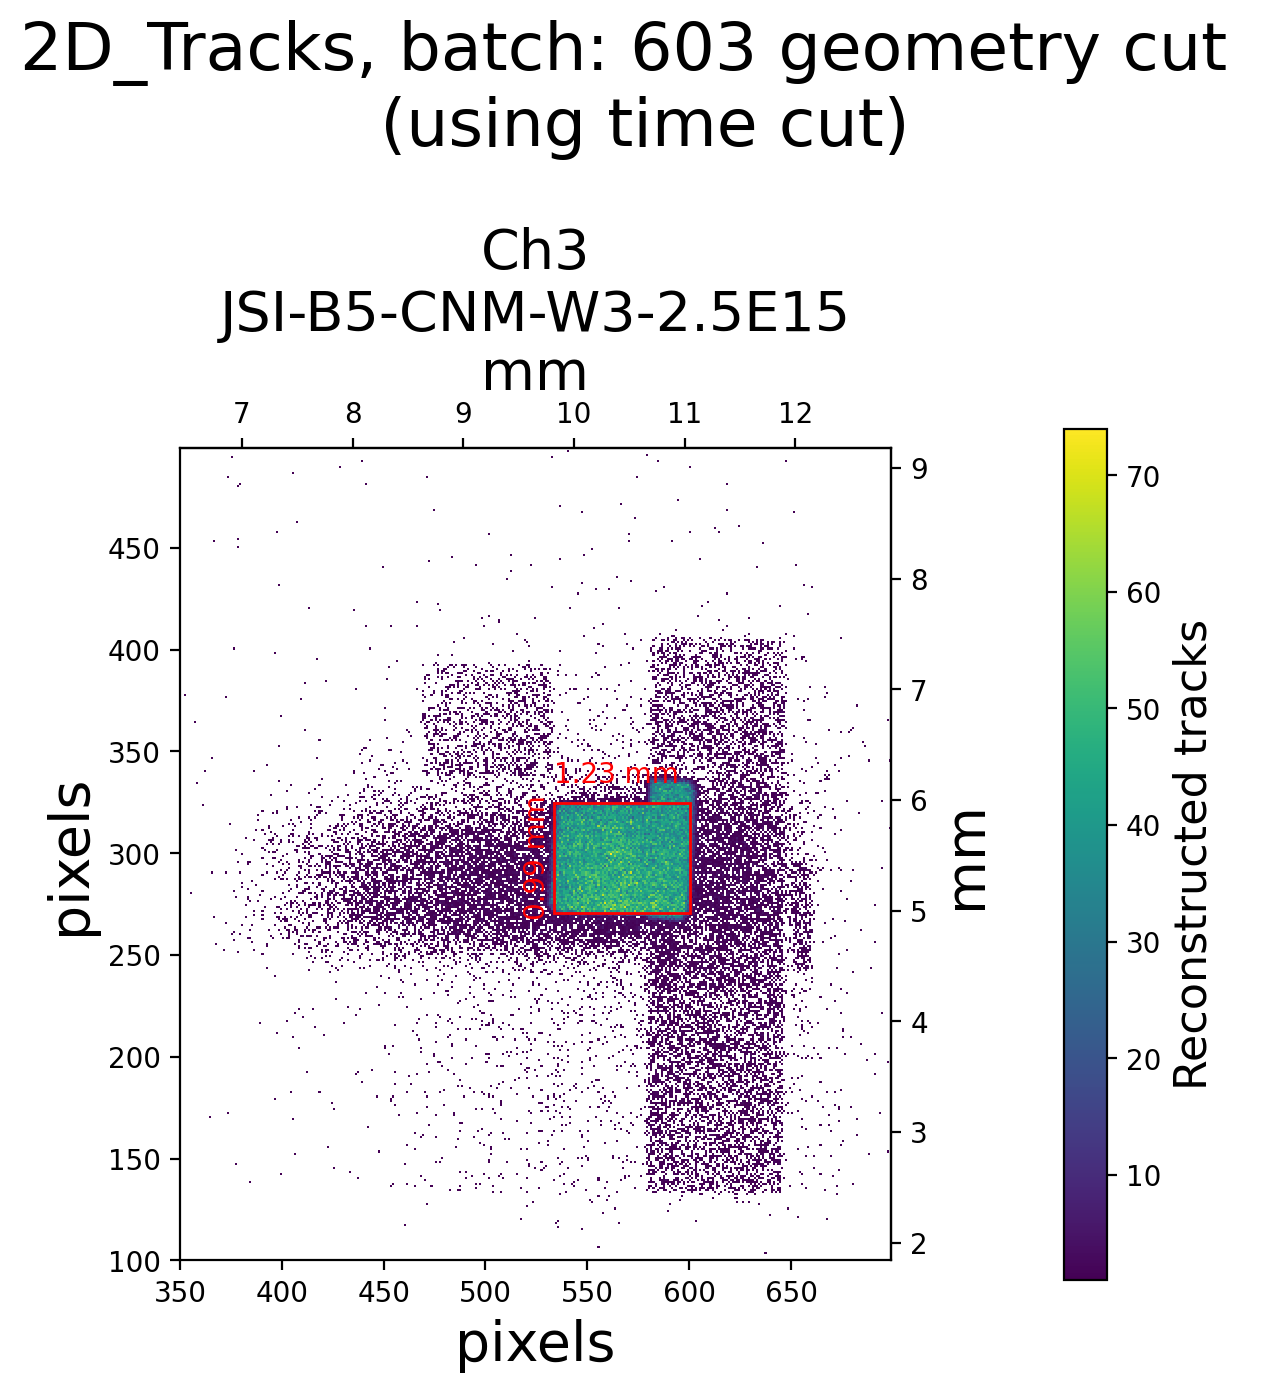
\includegraphics[width=.45\linewidth]{Images/methods/2D_Tracks_603_S2 highlight geometry cut (using time).png}
        \label{fig:time_cut_highlight}}
    \captionsetup{width=\captionwidth}
    \caption{Example of a different sensor (\textbf{irradiated}), for which the previous \textit{pulse height cut} became impractical (left), but using \textit{time cut} yielded a reasonable outline of the pad (right)}
\end{figure}

\subsection{Quality cuts validation}

To qualitatively confirm the soundness of the cuts performed, we plotted the density distribution of events of \(\boldsymbol{\Delta t}\) vs \textbf{pulse height} (Figures~\ref{fig:time_pulseHeight_nocut} and \ref{fig:time_pulseHeight_center}). The left plot shows all the available tracks, the right plot shows only the tracks that pass through the smaller central area of the DUT (a square of \(0.5\times0.5\si{mm^2}\) explained in Section~\ref{sec:geometry_cut}).

The plot on the right shows a narrow selection of events very likely to be a real signal (as they are guaranteed to have passed through the sensor). By comparing it with the plot on the left it can be noticed that a horizontal cut (\nameref{subsec:pulseHeight_cut}) and two vertical cuts (\nameref{subsec:time_cut}) provide indeed a good filter for physically meaningful events. 


\begin{figure}[h!tbp]
    \centering
    \subfloat[Density plot of all the event without any cuts applied. The red line and the green line show where \textit{pulse height cut} and \textit{time cut} would be applied, respectively.]{
        \includegraphics[width=.45\linewidth]{Images/methods/Time_pulseHeight_401_S1_with_info.png}
        \label{fig:time_pulseHeight_nocut}}
    \hfill
    \centering
    \subfloat[Density plot selecting only tracks passing through the central \(0.5\times0.5\si{mm^2}\) area of the pad.]{
        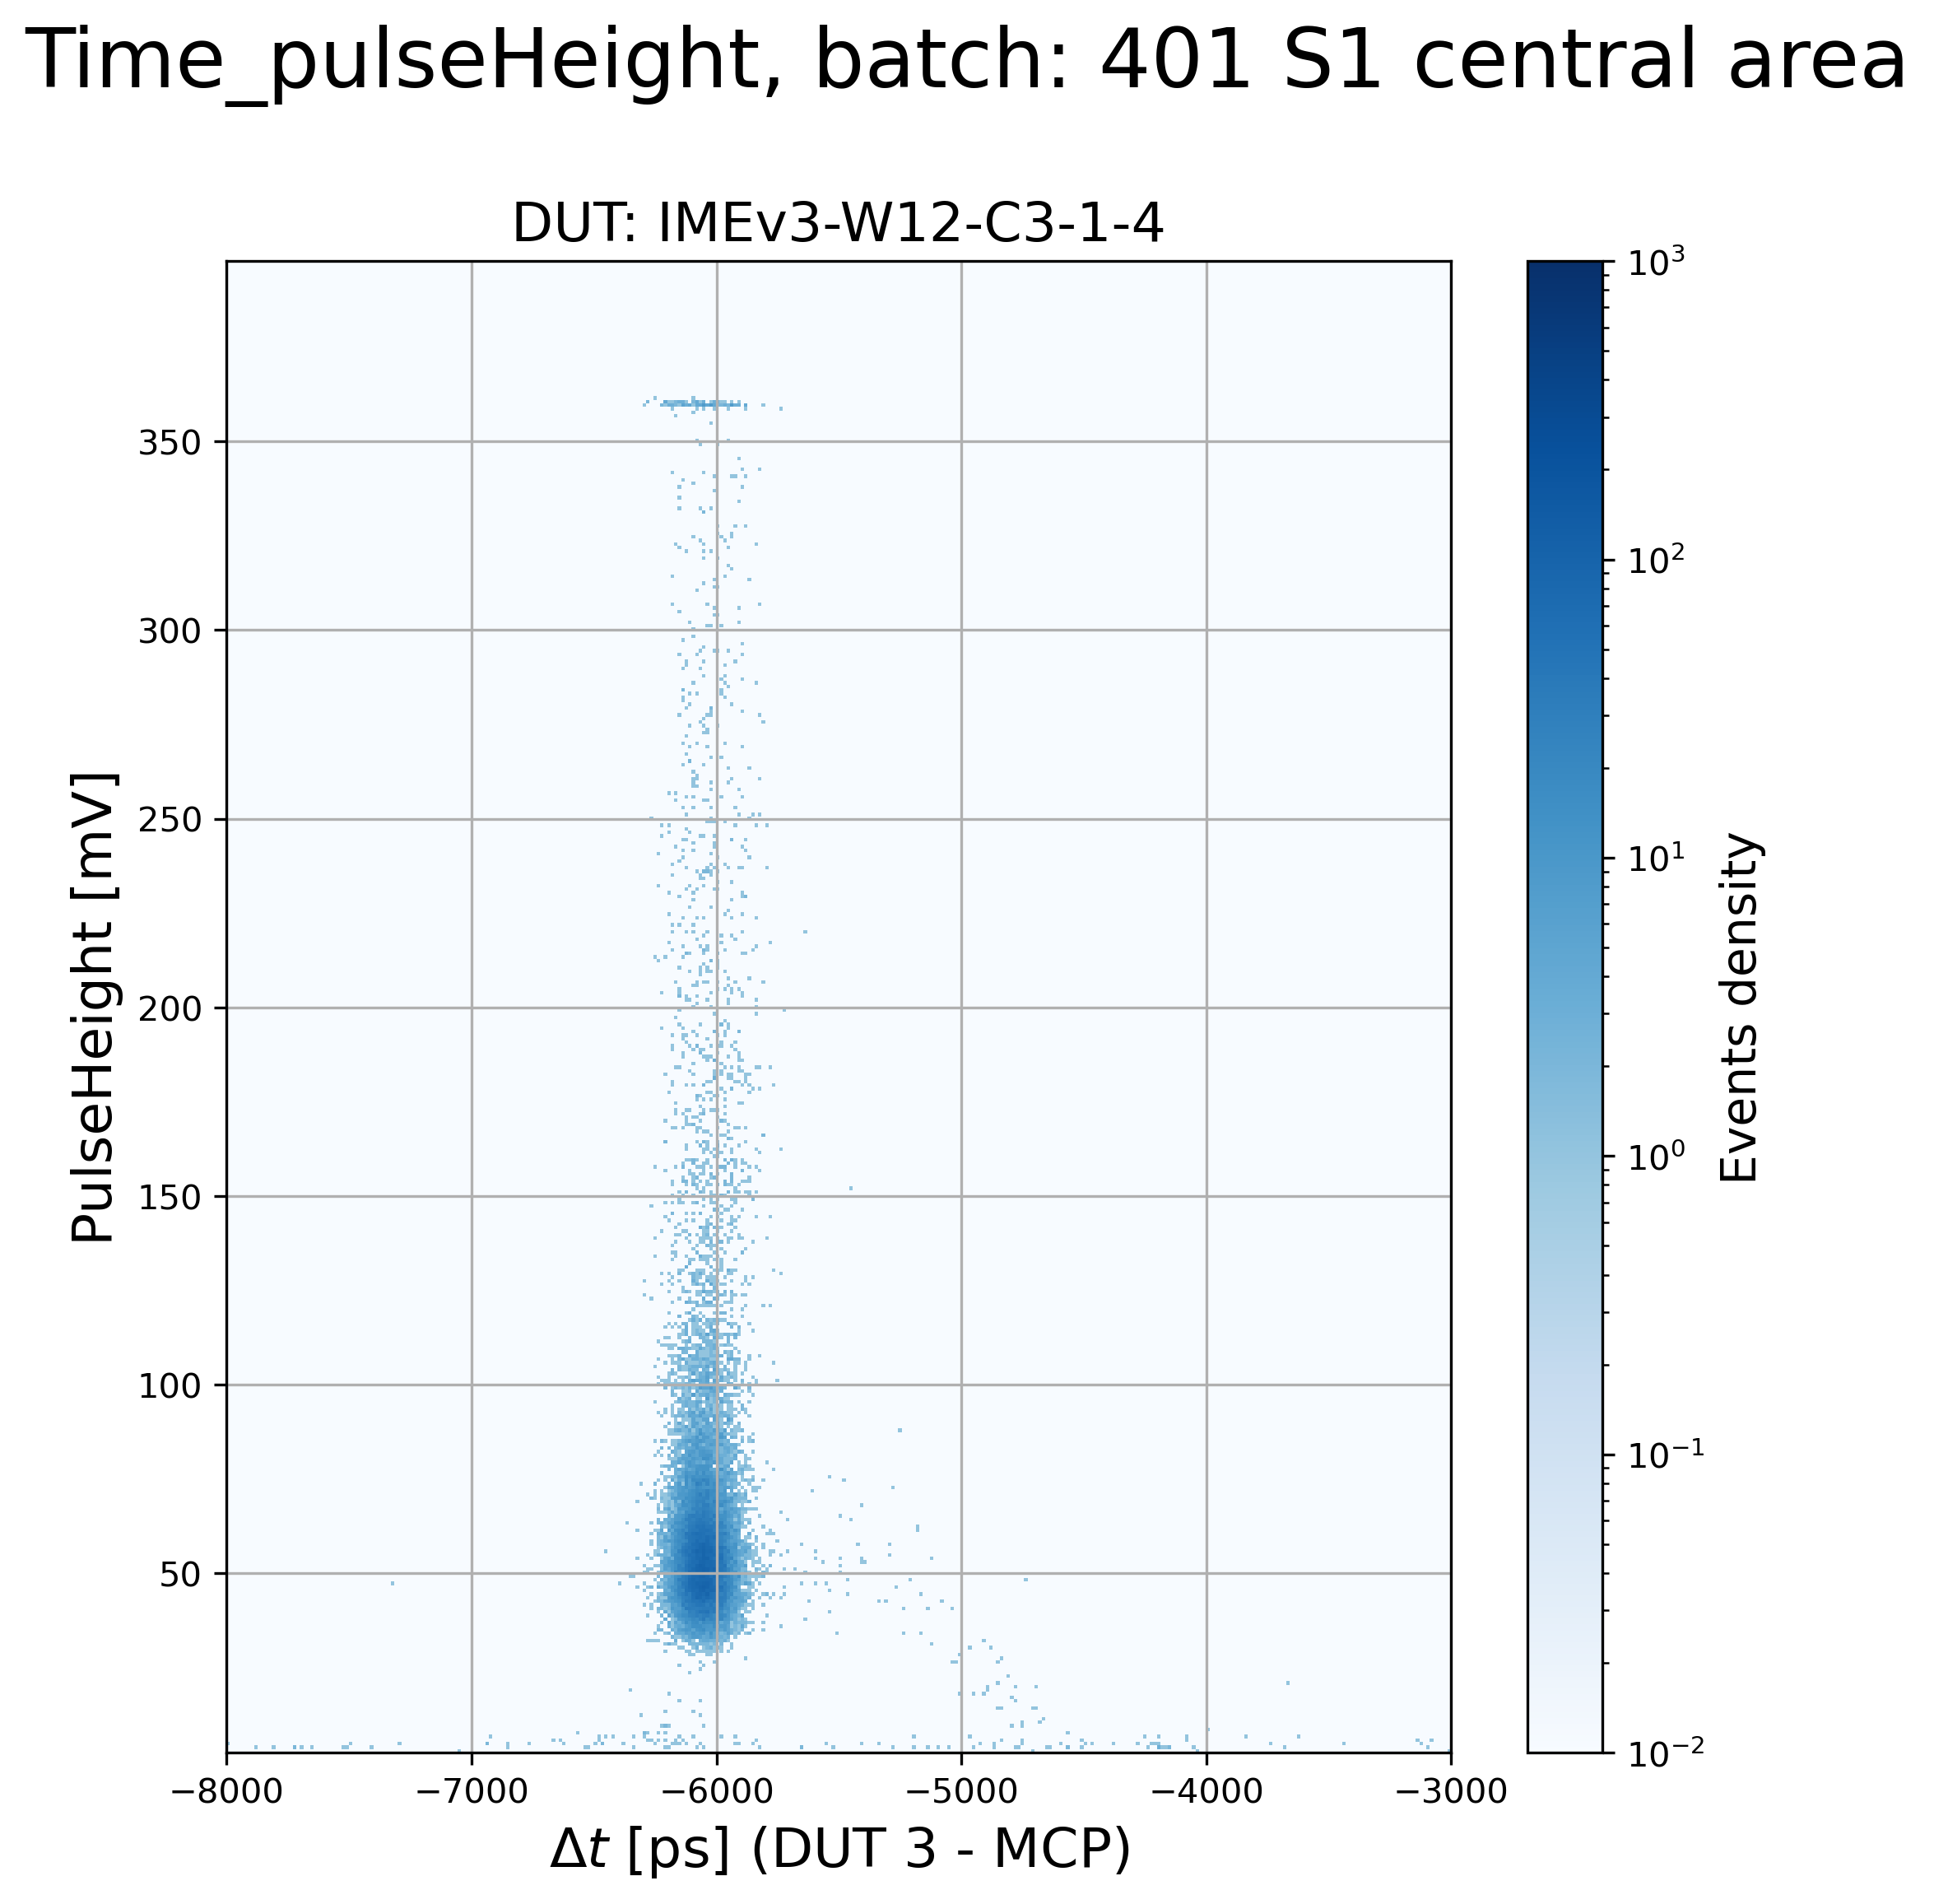
\includegraphics[width=.5\linewidth]{Images/methods/Time_pulseHeight_401S1 central area.png}
        \label{fig:time_pulseHeight_center}}
    \captionsetup{width=\captionwidth}
        \caption{Density plot of events when no cuts are applied (left) and when only a central square in the sensor is selected (right). The comparison between the two plots validates our choices made for quality cuts.}
\end{figure}


\section{Collected charge}\label{sec:methods_collected_charge}

A central goal of this study was to measure the distribution of the charge collected by the pads and verify their correspondence with the theoretical distribution: a convolution of a Gaussian and a Landau distribution (Appendix \ref{sec:vavilov_vs_landau_distribution}).

To achieve this, all the quality cuts defined in Section \ref{sec:qualtiy_cuts} were applied, and a fit was carried out using an implementation of the Gaussian*Landau convolution provided by the ROOT framework~\cite{Brun:1997pa} (Figure~\ref{fig:charge_ROOT_fit}).

The collected charge of a sensor is defined as the most probable value (MPV) of the charge, i.e. the highest point in the distribution.

\begin{figure}[h!tbp]
    \centering
    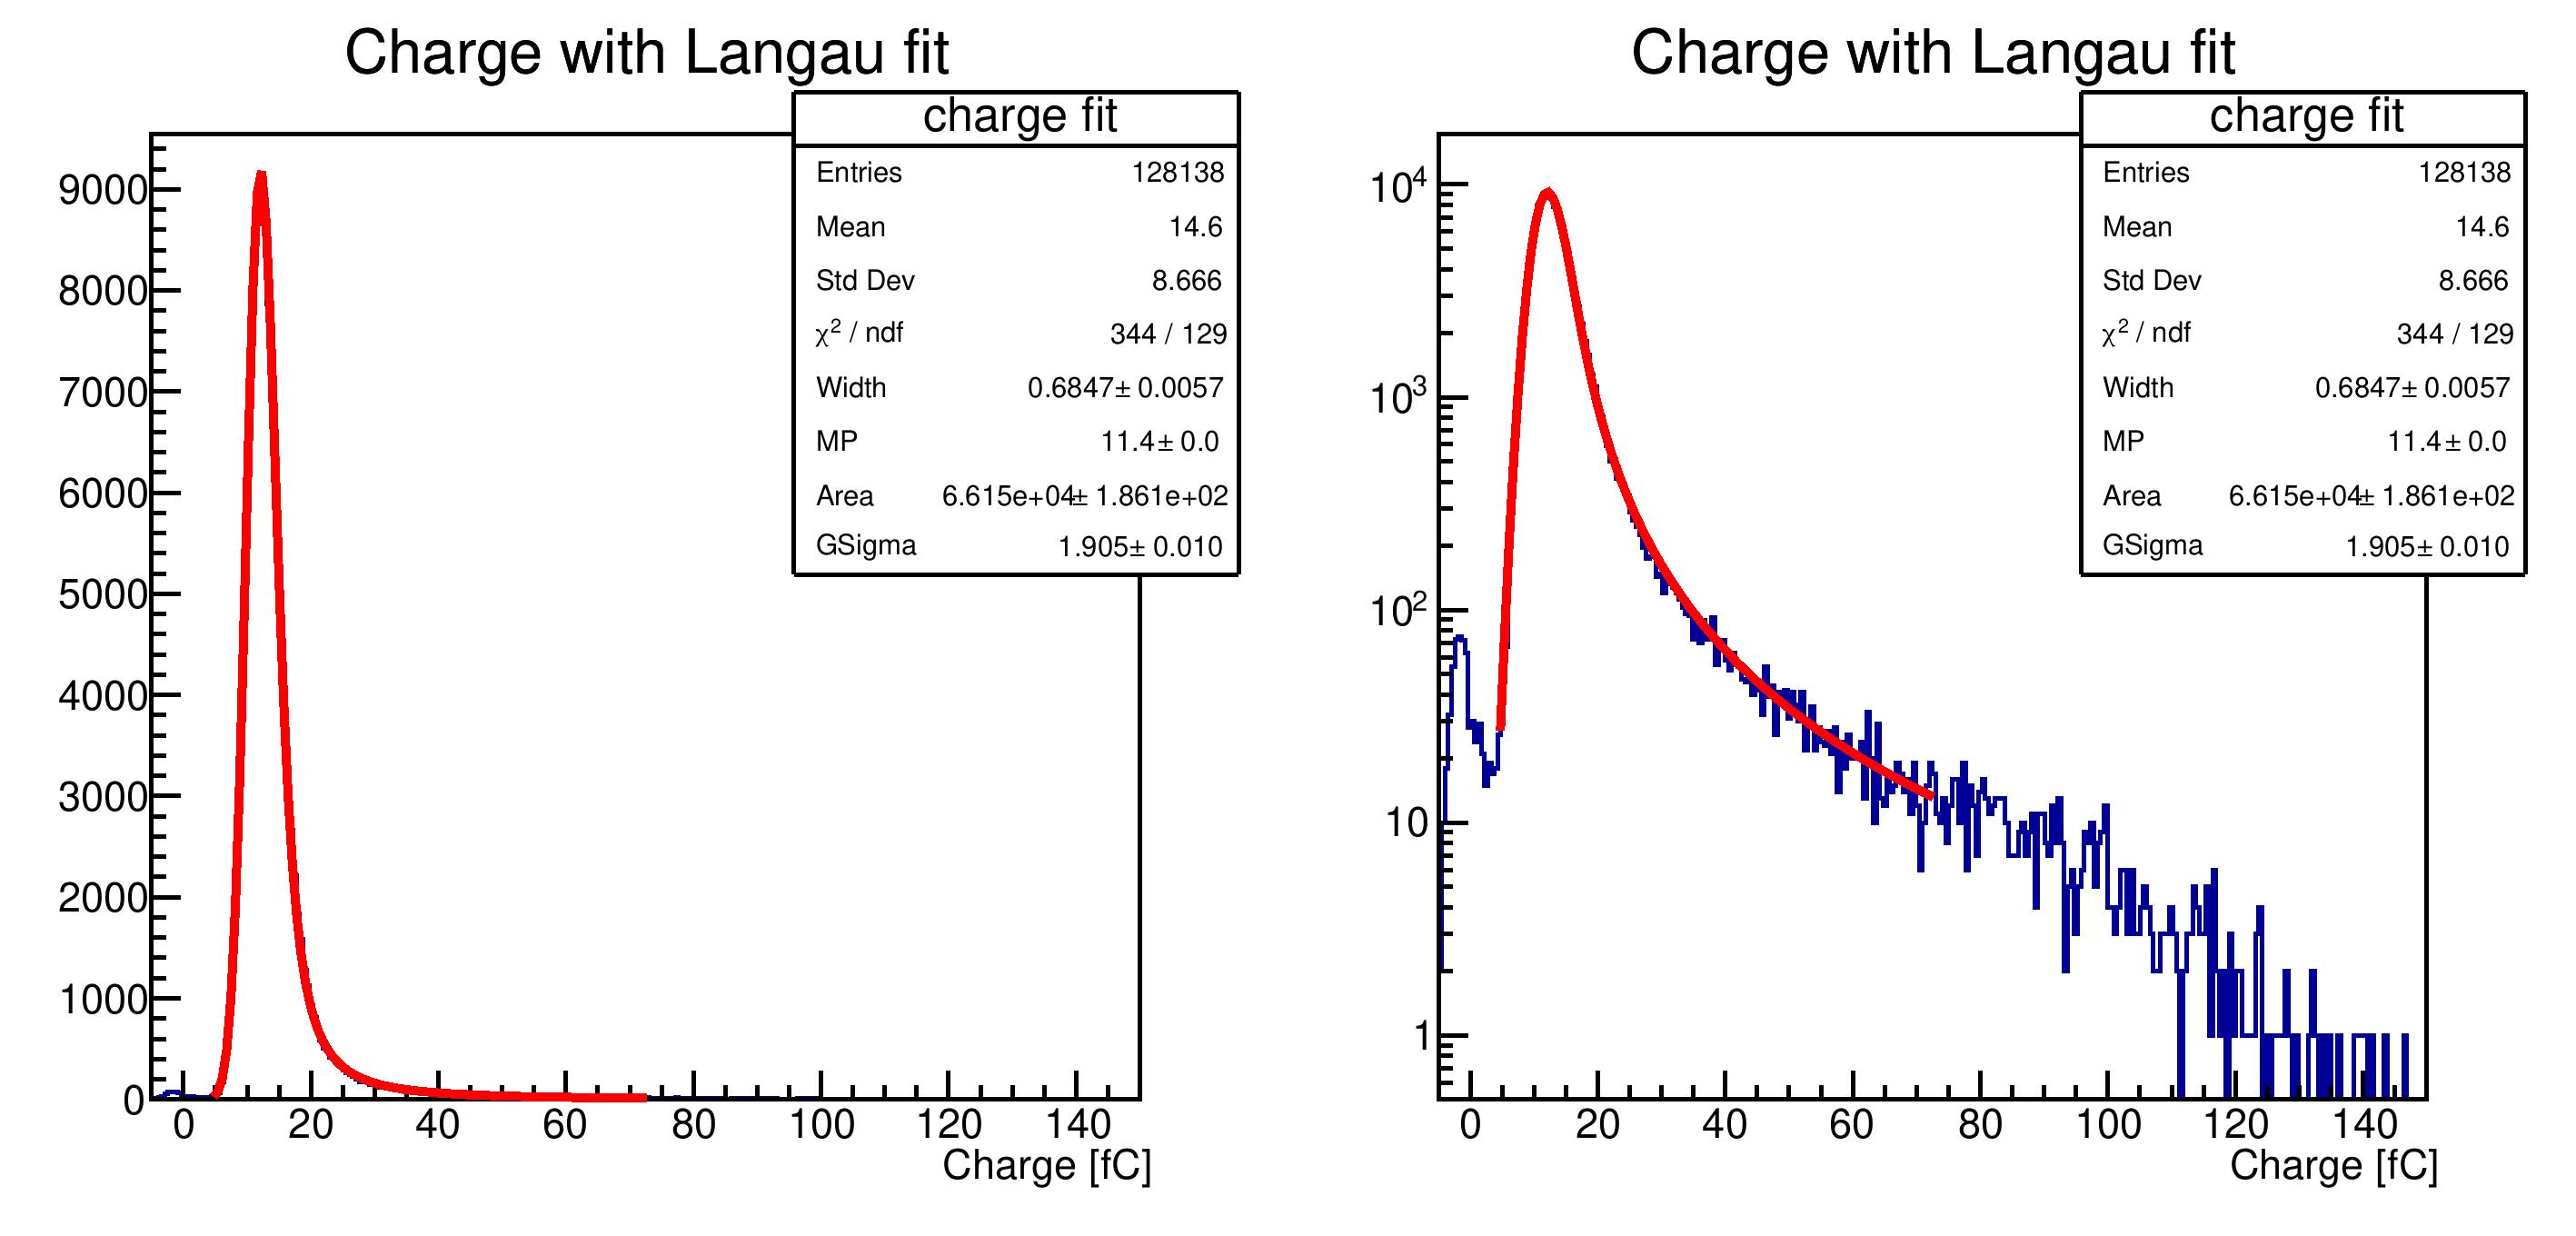
\includegraphics[width=1\linewidth]{Images/charge_plots/charge_data_all_cuts_401_S1_3_Charge_fit_ROOT_double_plot.png}
    \captionsetup{width=\captionwidth}
    \caption{Fit of the charge distribution (red) carried out with ROOT. On the right it is shown the same plot in logarithmic scale, to highlight the extra noise at \(\approx 0\).}
    \label{fig:charge_ROOT_fit}
\end{figure}

\subsubsection{Gain}
% charged particle in 50 um of silicon produce ~0.52 fC of charge or 3280 e-h pairs
The gain is obtained by dividing the most probable value of the collected charge by the expected charge from a minimum ionizing particle (MIP) in a silicon sensor without gain. For a \qty{50}{\micro\meter} thick sensor, this value is \(3280\) e-h pairs, equivalent to \qty{.52}{\femto\coulomb} \cite{meroli_energy_loss2011}.

\subsubsection{Extra noise}
Despite all the trimming to the data, a noticeable part of the noise centered at \(\approx 0\) could not be removed. We could not pinpoint the origin of this extra noise, but a lot of factors could contribute to it: track reconstruction, other electronic noise etc.
Considering this point, the fit was performed in a smaller interval, avoiding the noise (Figure~\ref{fig:charge_ROOT_fit}). The left limit was fixed at \(4\si{fC}\), as this is also the lowest signal that the electronic board is able to measure, the right limit was adjusted to include only bins with significant amount of data (and account for the \nameref{subsec:tail_discrepancies}, described in Appendix).

%%% maybe I can put a table to show which cuts I applied to which variables


\section{Efficiency}\label{sec:methods_efficiency}

The efficiency (\(\epsilon\)) was defined as the total number of tracks with charge larger than a certain \textit{threshold charge} divided by the total number of reconstructed track (\textbf{after} quality cuts had been applied).

% \begin{equation*}
%     \text{Efficiency} = \frac{\text{Tracks with } q>Q_{threshold}}{\text{Total tracks}}  \, .
% \end{equation*}

\begin{equation*}
    \epsilon = \frac{\text{Tracks with } q>Q_{threshold}}{\text{Total tracks}}  \, .
\end{equation*}

The threshold charge \(Q_{threshold}\) was chosen to be \(4\si{fC}\), which corresponds to the limit of sensitivity of the ASIC.

Before measuring the overall efficiency of the sensors, we applied a \textit{time cut} (as described in \nameref{subsec:time_cut}). Additionally, we elected to restrict the calculation to the smaller \textit{central area} of \(0.5\times0.5\si{mm^2}\) defined earlier in \nameref{sec:geometry_cut}. This area can be seen highlighted in red in Figure~\ref{fig:efficiency_2D_plot}, which also shows how the efficiency value computed for each individual squared binning of the surface.

Finally, the total efficiency was computed with different values of \textit{threshold charge} to obtain the plot in Figure~\ref{fig:efficiency_depending_threshold}, which shows that (in this example) the value remains constant well after the chosen threshold of \(4\si{fC}\).

\begin{figure}[h!tbp]
    \centering
    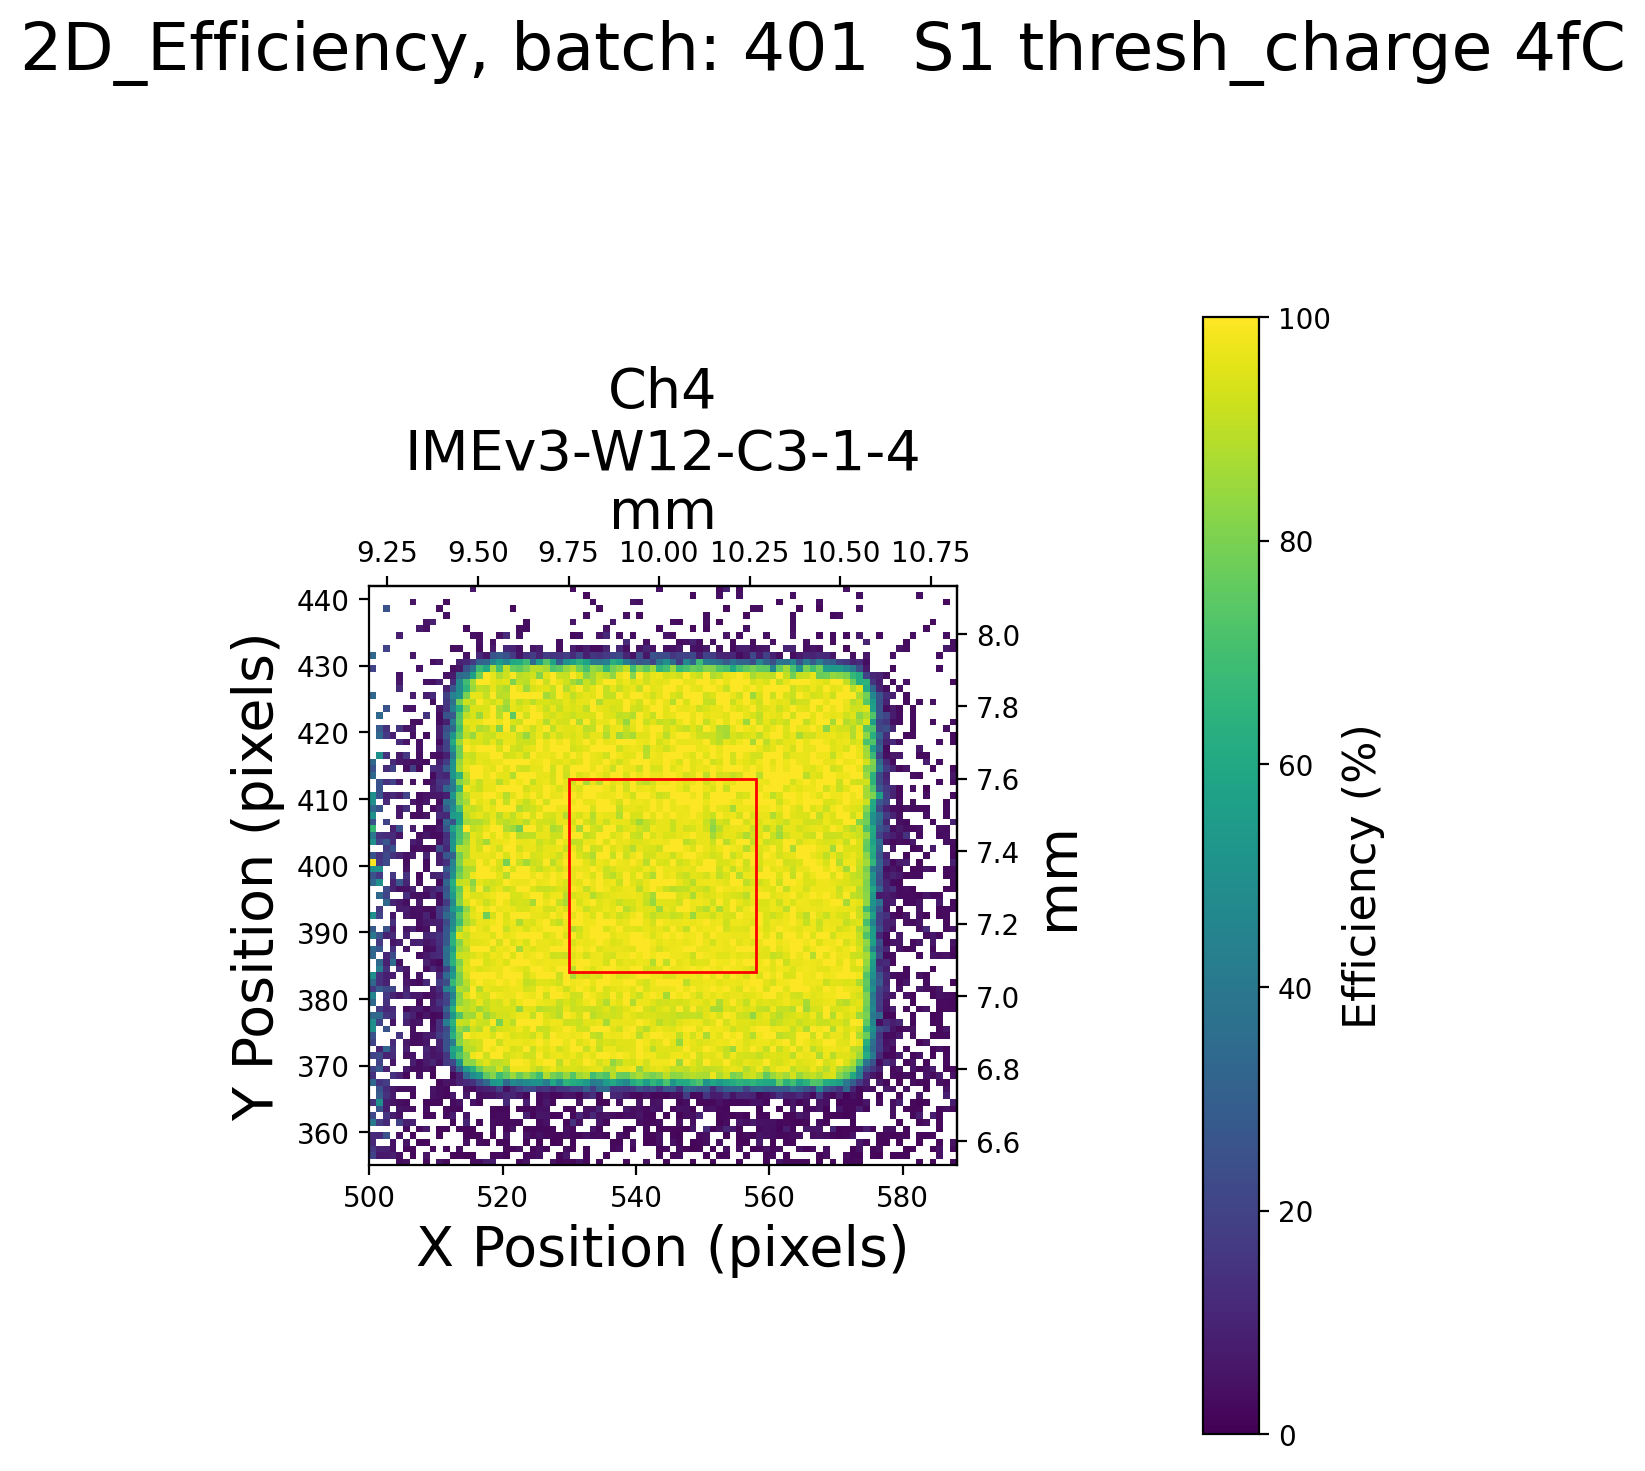
\includegraphics[width=0.7\linewidth]{Images/efficiency_plots/2D Efficiency_401_S1_with_center_highlight_DUTs_3.png}
    \captionsetup{width=\captionwidth}
    \caption{2D histogram plot of efficiency (per squared bin) and \textit{central area cut} highlighted in red.}
    \label{fig:efficiency_2D_plot}
\end{figure}

\begin{figure}[h!tbp]
    \centering
    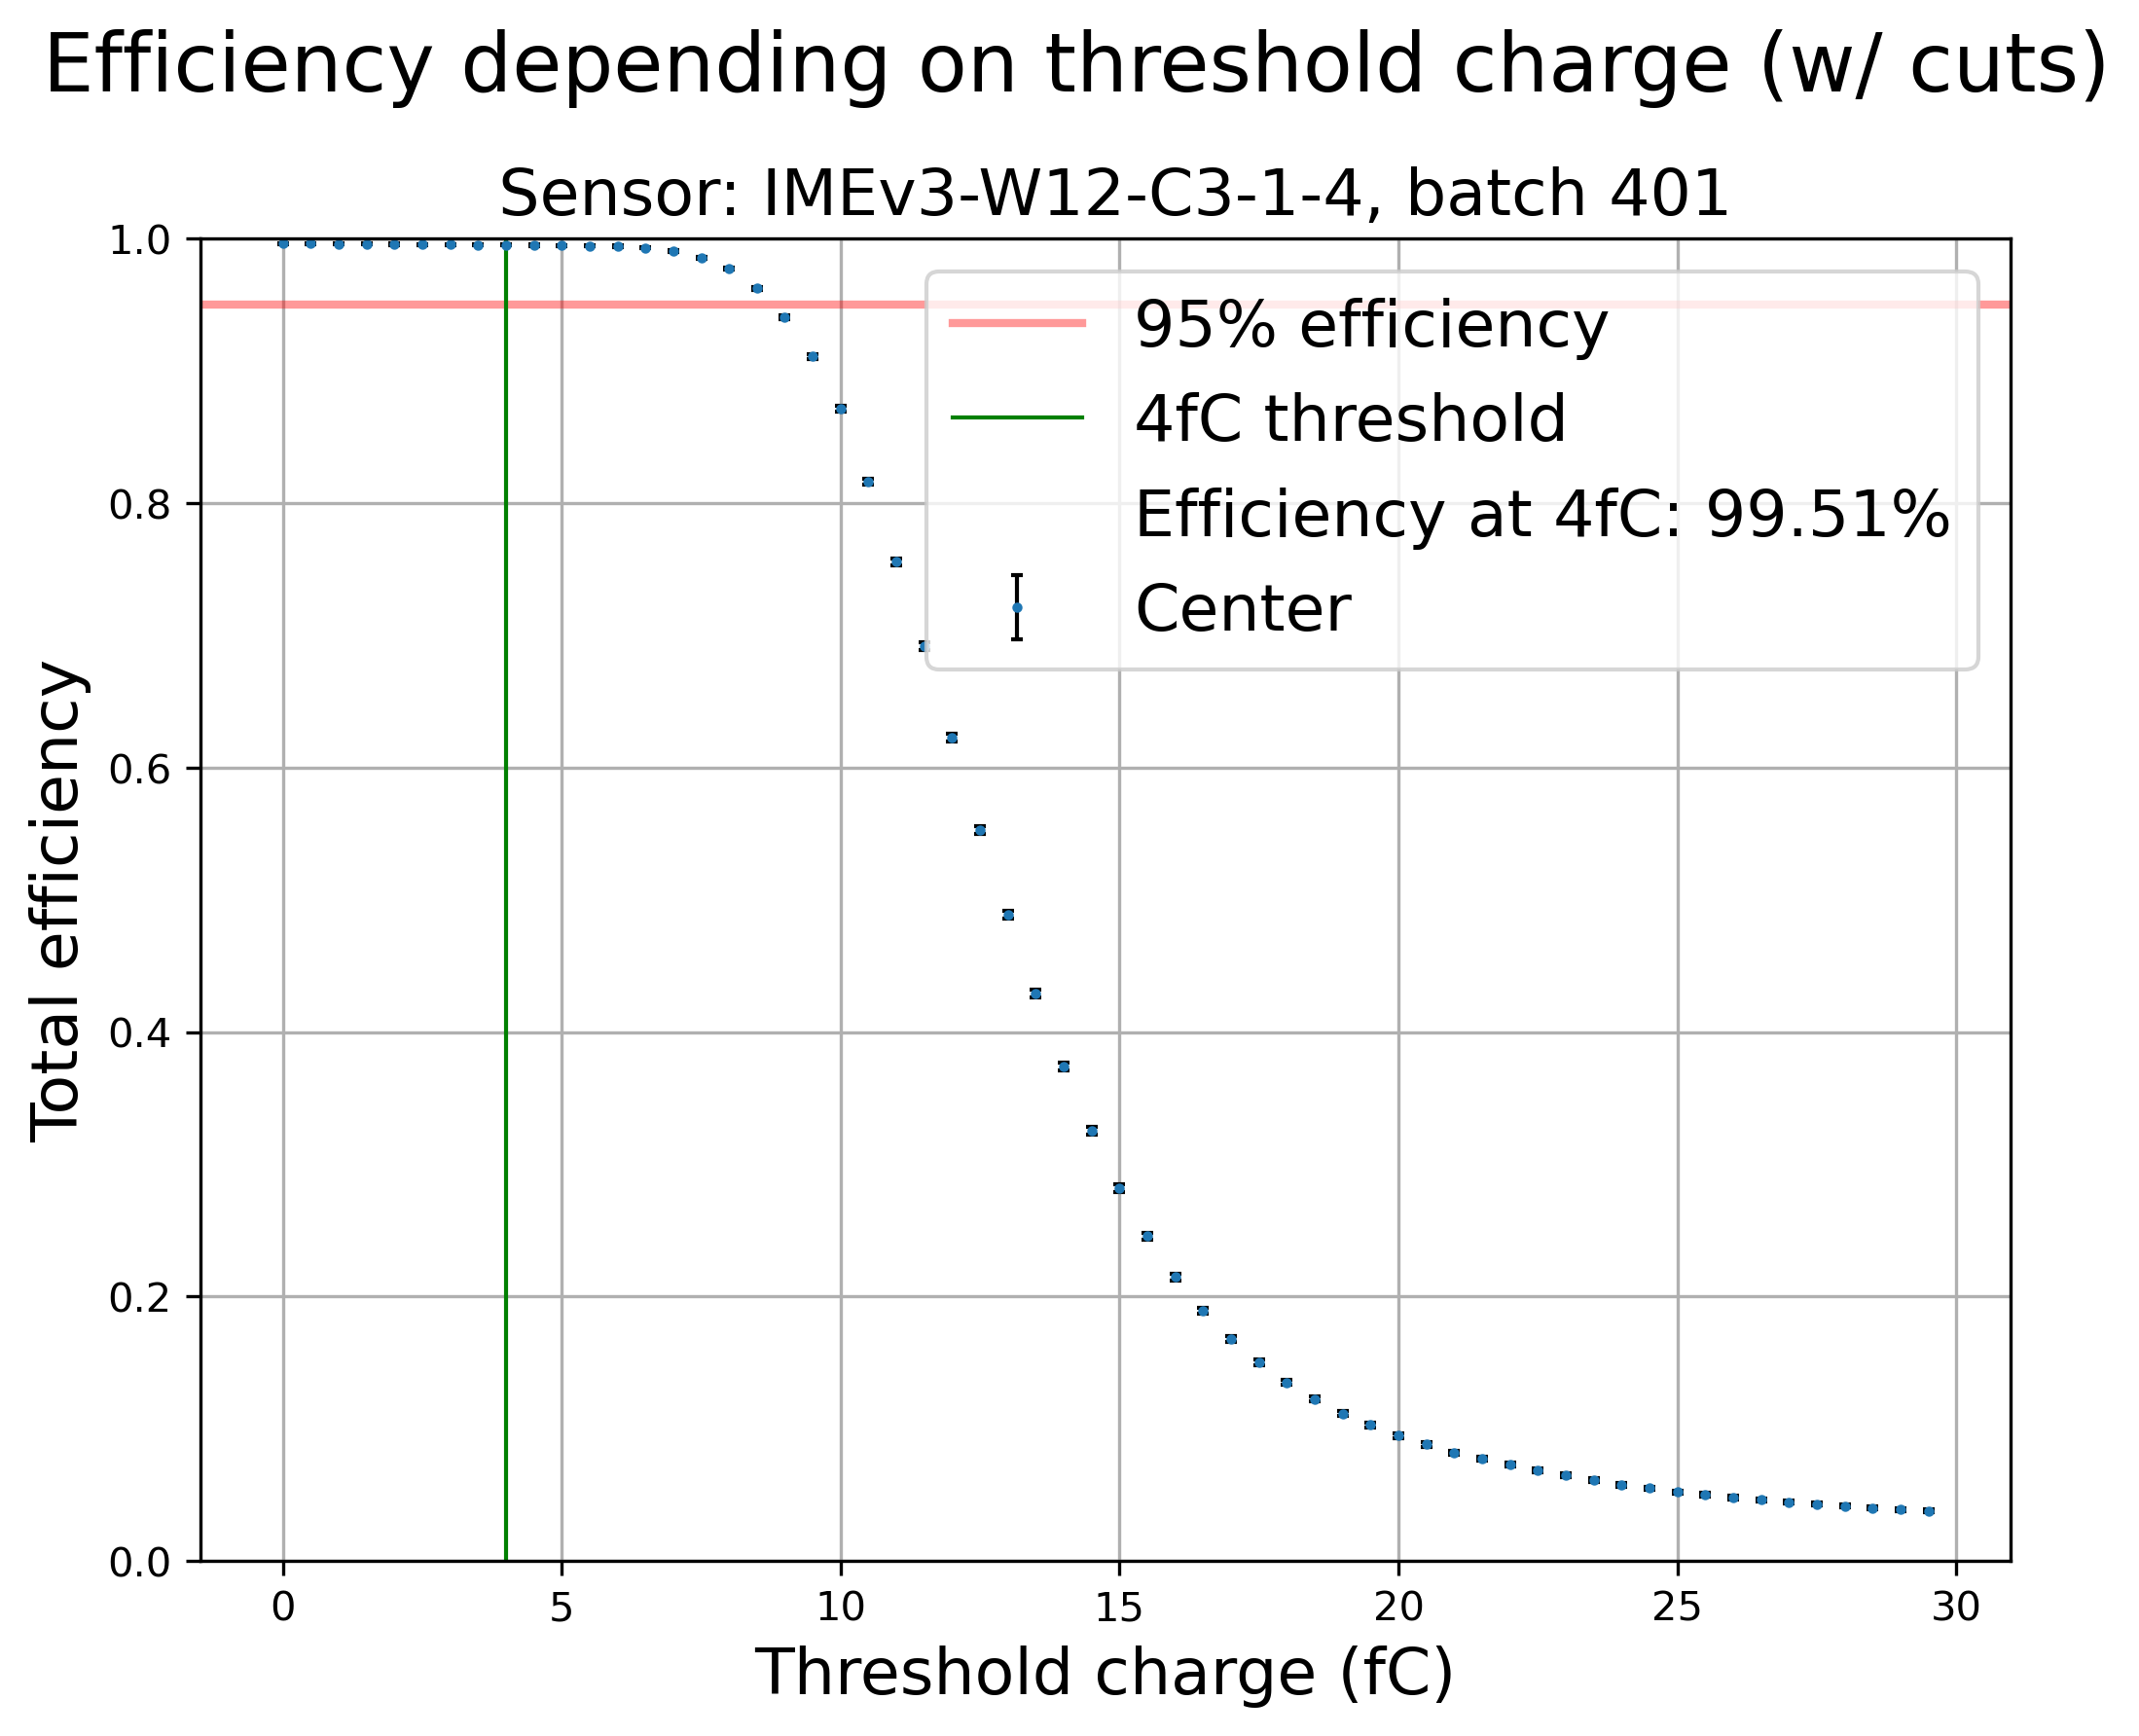
\includegraphics[width=0.5\linewidth]{Images/efficiency_plots/Efficiency depending on threshold charge (with cuts) batch 401 S1.png}
    \caption{Total efficiency when changing the threshold value, ensuring that there is a large plateau of high efficiency.}
    \label{fig:efficiency_depending_threshold}
\end{figure}


\section{Time Resolution}\label{sec:methods_time_resolution}

The difference of times of arrival between the DUT and the MCP was fitted with a normal distribution. The standard deviation of said distribution corresponded to the time resolution of the DUT and MCP combined. Using simple error propagation, the time resolution of the DUT was computed: 

\begin{equation*}
    \begin{gathered}
    \sigma_{dut+MCP} = \sigma_{dut} \oplus \sigma_{MCP} \\
    \downarrow \\
    \sigma_{dut+MCP}^2 = \sigma_{dut}^2 + \sigma_{MCP}^2 \\
    \sigma_{dut} = \sqrt{\sigma_{dut+MCP}^2-\sigma_{MCP}^2}  \, .
    \end{gathered}
\end{equation*}

For this sensor (Figure~\ref{fig:time_resolution_plot}) the final time resolution was \(\sigma_{dut} = 49.38\pm0.81\si{\ps} \)

\begin{figure}[h!tbp]
    \centering
    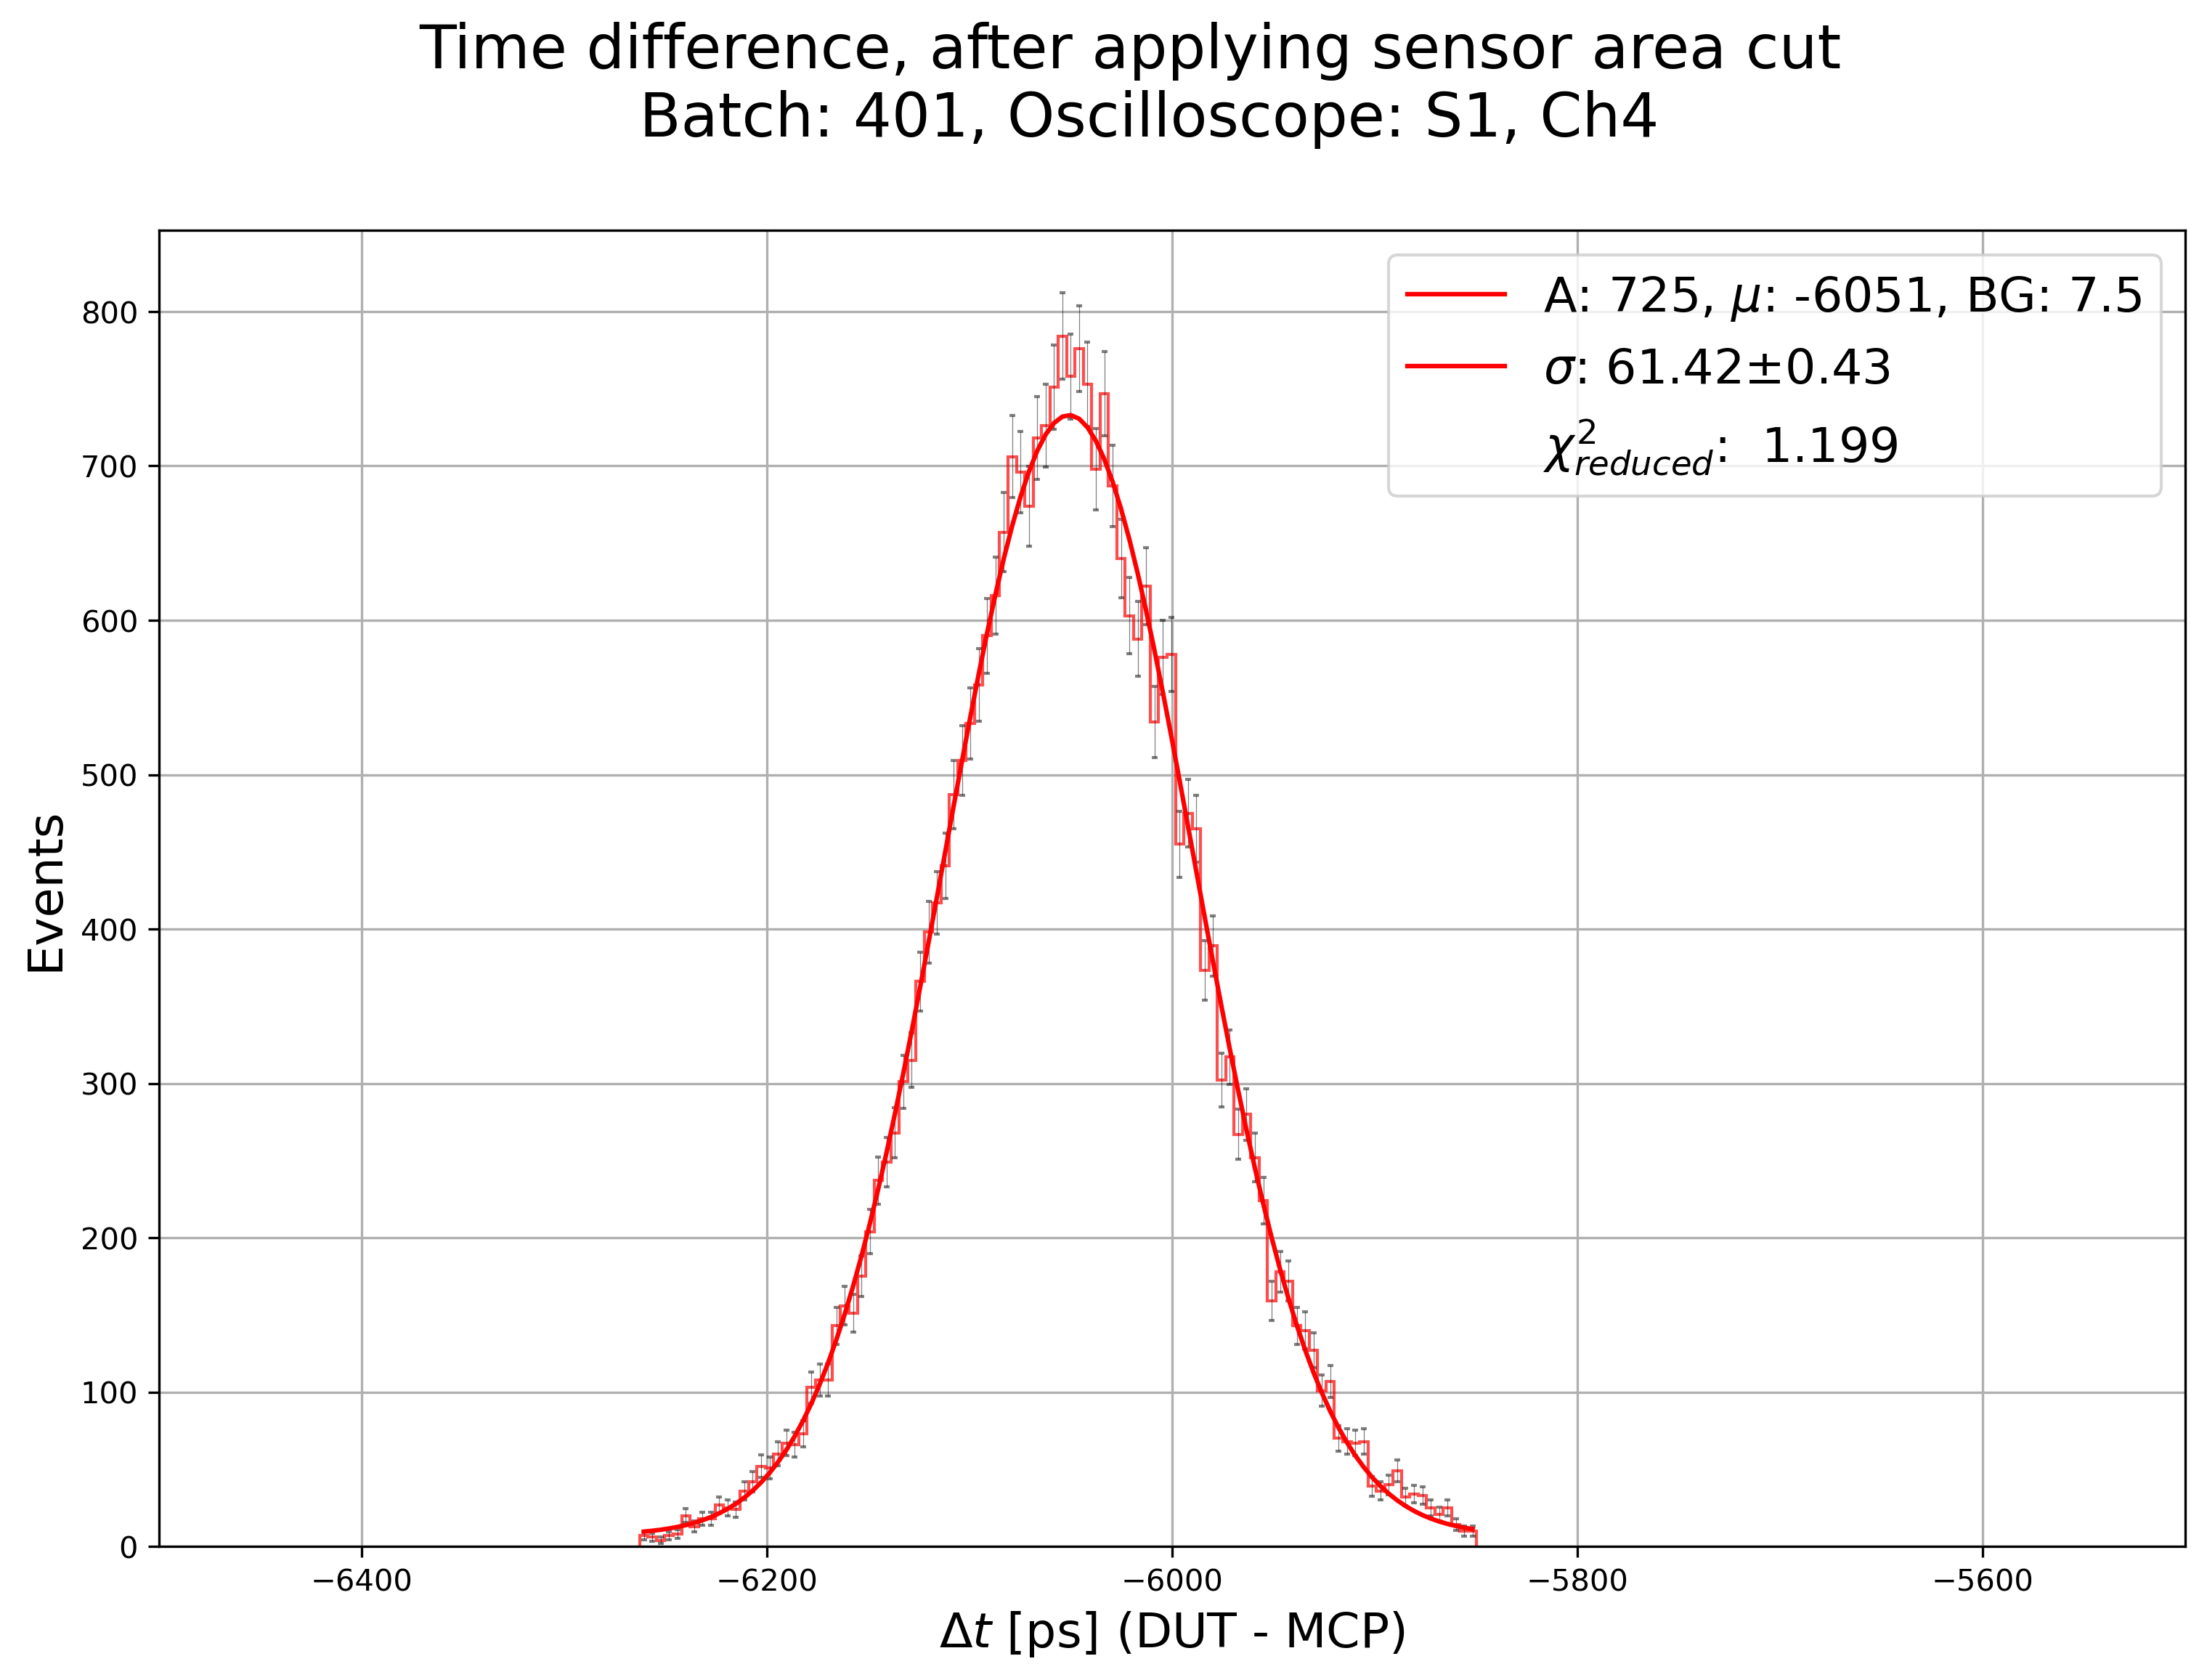
\includegraphics[width=0.7\linewidth]{Images/time_resolution_plots/time_difference_401_S1_zoomed_and_gauss_fit_with_cuts_central_area_DUTs_3.png}
    \captionsetup{width=\captionwidth}
    \caption{Gaussian fit of \(\Delta t\) to find the time resolution (\(\sigma\)), the error bars are the statistical poissonian error (\(y_{err}=\sqrt{N}\)).}
    \label{fig:time_resolution_plot}
\end{figure}




\chapter{Results}\label{chap:results}

The main goal of this analysis was to quantify key metrics of the performance of LGAD sensors. In particular, we analyzed the collected charge, the time resolution and the efficiency at the temperature of \qty{-30}{\degreeCelsius}, which will be the temperature of the detector in operation. We compared the results between unirradiated and differently irradiated sensors to test whether the requirements at start and end of life were satisfied. The sensors were also studied at angles between \qty{0}{\degree} and \qty{14}{\degree} relative to the beam direction, in line with the HGTD's expected pseudorapidity coverage: between \(2.4\) and \(4\), which corresponds to incident angles of \qtyrange{2}{10}{\degree}.

Additionally, some other properties and effects that arose during the analysis were also investigated. Such as, signal coming from neighbouring pads, noise coming from outside the gain layer of the pads, and properties of the region lying between two adjacent pads. Certain anomalies were also successfully explained, and the root cause was found in the incorrect voltage range set on an oscilloscope, which caused pulses to be "clipped" below a specific threshold. Moreover, due to a temporary malfunction of the cooling box, one batch of data showed neatly the sensitivity of LGADs to temperature variations.

\section{Main Results}

\begin{figure}[h!tbp]
    \centering
    \includegraphics[width=.9\linewidth]{Images/Results/Irradiated/IME_voltage_charge_.png}
    \captionsetup{width=\captionwidth}
    \caption{Overview of voltage vs collected charge for all the studied sensors from IME. \(\Phi\) is the radiation dose of each sensor in neutron-equivalent fluence.}
    \label{fig:irradiated_IME_voltage_charge}
\end{figure}


\begin{figure}[h!tbp]
    \centering
    \includegraphics[width=.9\linewidth]{Images/Results/Irradiated/IME_voltage_time_resolution_.png}
    \captionsetup{width=\captionwidth}
    \caption{Overview of voltage vs time resolution.}
    \label{fig:irradiated_IME_voltage_time_res}
\end{figure}

The most important properties of the sensors are:

\begin{itemize}
    \item Collected change: the most probable value (MPV) of the Landau*Gaussian convolution (Section~\ref{sec:methods_collected_charge}).
    \item Time resolution: the spread of the Gaussian distribution of the Time of Arrivals (Section~\ref{sec:methods_time_resolution}).
    \item Efficiency: the fraction of incident particles that produce a detectable signal in the sensor. (Section~\ref{sec:methods_efficiency}).
\end{itemize}

Overall all sensors behaved as expected: their collected charge increased with higher bias voltage and decreased with higher radiation dose (fluence), and most of them satisfied the HGTD's requirements.

\subsection{Irradiated samples performance}

\subsubsection{IME}

The sensors in the IME group were further split depending on versions and types, to enable more meaningful comparisons between devices with similar characteristics. More specifically:

\begin{itemize}
    \item IMEv3-W12: 2\(\times\)2 array unirradiated, 1\(\times\)3 array unirradiated and 2\(\times\)2 array at \qty{1.5e15}{\neutroneq}.
    \item IMEv2-W7: single pad at \qty{1e14}{\neutroneq} and single pad at \qty{6.5e14}{\neutroneq}.
    \item IMEv3-W16: single pad at \qty{8e14}{\neutroneq} and single pad at \qty{2.5e15}{\neutroneq}.
\end{itemize}

%%% IMEv3-W12, 0 and 
\begin{figure}[h!tbp]
    \centering
    \subfloat[Voltage vs Charge.]{
        \includegraphics[width=.49\linewidth]{Images/Results/Irradiated/IMEv3-W12_voltage_charge_irradiated.png}
        \label{fig:IMEv3-W12_voltage_charge}}
    \hfill
    \subfloat[Voltage vs Time resolution]{
        \includegraphics[width=.47\linewidth]{Images/Results/Irradiated/IMEv3-W12_voltage_time_resolution_irradiated.png}
        \label{fig:IMEv3-W12_voltage_time_res}}
    \vfill
    \subfloat[Voltage vs Efficiency]{
        \includegraphics[width=.47\linewidth]{Images/Results/Irradiated/IMEv3-W12_voltage_efficiency_irradiated.png}
        \label{fig:IMEv3-W12_voltage_efficiency}}
    \captionsetup{width=\captionwidth}
    \caption{IMEv3-W12. The non irradiated sensors (both the 2\(\times\)2 array and the 1\(\times\)3 array) had sufficiently high collected charge at all tested bias voltages, while the time resolution was just short of the \qty{35}{\pico\second} target in the case of the 2\(\times\)2 array, although this is likely to be solved with higher applied voltage. The lack of data for higher voltages was due to erroneous batches. It should be noted that the two pads of the 1\(\times\)3 array had significant and consistent discrepancies in charge and time resolution, presumably due to differences at the manufacturing stage. The sensors at \qty{1.5e15}{\neutroneq} had very good performance overall and still reached the target time resolution of beginning of operations (\qty{35}{\pico\second}) at \(\simeq60\%\) of the total expected dose. The efficiency satisfied the \(95\%\) goal above \(\approx\qty{400}{\volt}\).}
\end{figure}

\begin{figure}[p!htb]
    \centering
    \subfloat[Voltage vs Charge]{
        \includegraphics[width=.47\linewidth]{Images/Results/Irradiated/IMEv2-W7_voltage_charge_irradiated.png}
        \label{fig:IMEv2-W7_voltage_charge}}
    \hfill
    \subfloat[Voltage vs Time resolution]{
        \includegraphics[width=.45\linewidth]{Images/Results/Irradiated/IMEv2-W7_voltage_time_resolution_irradiated.png}
        \label{fig:IMEv2-W7_voltage_time_res}}
    \vfill
    \begin{minipage}[c]{.47\linewidth}
    \subfloat[Voltage vs Efficiency]{
        \includegraphics[width=.95\linewidth]{Images/Results/Irradiated/IMEv2-W7_voltage_efficiency_irradiated.png}
        \label{fig:IMEv2-W7_voltage_efficiency}}
        % \captionsetup{width=\captionwidth}
    \end{minipage}
    \hfill
    \begin{minipage}[c]{.5\linewidth}
        \captionof{figure}{IMEv2-W7. For both fluences (\qty{1e14}{\neutroneq} and \qty{6.5e14}{\neutroneq}, i.e. low fluence) charge, time resolution and efficiency were within the targets for larger voltages. Although, the more heavily irradiated sensor showed a significant variation in the efficiency, which increased from \(\approx30\%\) up to \(\approx95\%\).}
\end{minipage}
\end{figure}

\begin{figure}[p!htb]
    \centering
    \subfloat[Voltage vs Charge]{
        \includegraphics[width=.47\linewidth]{Images/Results/Irradiated/IMEv3-W16_voltage_charge_irradiated.png}
        \label{fig:IMEv3-W16_voltage_charge}}
    \hfill
    \subfloat[Voltage vs Time resolution]{
        \includegraphics[width=.45\linewidth]{Images/Results/Irradiated/IMEv3-W16_voltage_time_resolution_irradiated.png}
        \label{figIMEv3-W16_voltage_time_res}}
    \vfill
    \begin{minipage}[c]{.47\linewidth}
    \subfloat[Voltage vs Efficiency]{
        \includegraphics[width=.95\linewidth]{Images/Results/Irradiated/IMEv3-W16_voltage_efficiency_irradiated.png}
        \label{fig:IMEv3-W16_voltage_efficiency}}
    \end{minipage}
    \hfill
    \begin{minipage}[c]{.5\linewidth}
    \captionof{figure}{IMEv3-W16. The sensor at \qty{8e14}{\neutroneq} performed well overall, except for the batch at highest bias voltage, which saw a small but unexpected worsening of time resolution and efficiency. We investigated further the cause, but we were unable to pinpoint the exact source. The sensor at \qty{2.5e15}{\neutroneq}, corresponding to the end-of-life radiation dose, had a collected charge below the requirements, slightly below \qty{3}{\femto\coulomb} and very poor efficiency, but it showed satisfactory time resolution.}
\end{minipage}
\end{figure}

\FloatBarrier

\subsubsection{USTC}

The data from the USTC sensor was the most affected by missing and erroneous batches, as the data from the irradiated sensor was not available.

\begin{figure}[h!tbp]
    \centering
    \subfloat[Voltage vs Charge]{
        \includegraphics[width=.47\linewidth]{Images/Results/Irradiated/USTC_voltage_charge_.png}
        \label{fig:USTC_voltage_charge}}
    \hfill
    \subfloat[Voltage vs Time resolution]{
        \includegraphics[width=.45\linewidth]{Images/Results/Irradiated/USTC_voltage_time_resolution_.png}
        \label{fig:USTC_voltage_time_res}}
    \vfill
    \begin{minipage}[c]{.47\linewidth}
    \subfloat[Voltage vs Efficiency]{
        \includegraphics[width=.95\linewidth]{Images/Results/Irradiated/USTC_voltage_efficiency_.png}
        \label{fig:USTC_voltage_efficiency}}
    \end{minipage}
    \hfill
    \begin{minipage}[c]{.5\linewidth}
        \captionof{figure}{USTC. The sensor had very good collected charge and efficiency, albeit falling short of the time resolution aim. It also manifested evident differences between the two neighbouring pads. Unfortunately, the data of the irradiated USTC sensor was not available, so no comparison was possible.}
\end{minipage}
\end{figure}

\subsubsection{CNM}

The unirradiated sensors were used to measure the time resolution of the MCP (Section~\ref{sec:MCP_description}). They had already been tested before (as in \cite{Allaire:2018bof}) and they showed similar performance, with gain up to \qtyrange{40}{50}{}, and time resolution better than \qty{30}{\pico\second}. In this test beam they were also tested irradiated at two fluences: \qty{1.5e15}{\neutroneq} and \qty{2.5e15}{\neutroneq}.

\begin{figure}[h!tbp]
    \centering
    \subfloat[Voltage vs Charge]{
        \includegraphics[width=.47\linewidth]{Images/Results/Irradiated/CNM_voltage_charge_.png}
        \label{fig:CNM_voltage_charge}}
    \hfill
    \subfloat[Voltage vs Time resolution]{
        \includegraphics[width=.45\linewidth]{Images/Results/Irradiated/CNM_voltage_time_resolution_.png}
        \label{fig:CNM_voltage_time_res}}
    \vfill
    \begin{minipage}[c]{.47\linewidth}
    \subfloat[Voltage vs Efficiency]{
        \includegraphics[width=.95\linewidth]{Images/Results/Irradiated/CNM_voltage_efficiency_.png}
        \label{fig:CNM_voltage_efficiency}}
    \end{minipage}
    \hfill
    \begin{minipage}[c]{.5\linewidth}
        \captionof{figure}{CNM. The good performance of the unirradiated sensors was confirmed. At the highest expected radiation dose the sensor had an unexpected counter trend of time resolution, however, the two batches at lower voltages had a significantly lower amount of data available, potentially underestimating the error on the fit. Also, the efficiency (with a threshold of \qty{4}{\femto\coulomb}) did not reach \(30\%\) even at \qty{600}{\volt}.}
\end{minipage}
\end{figure}

\FloatBarrier 

\subsection{Angled samples performance}

When particles traverse a sensor at an angle, the effective path inside the volume of the sensor will be slightly larger (\(\approx3\%\) at \qty{14}{\degree}). For this reason, charge deposition will be greater and a small improvement in the performance is expected.
The sensors were studied with incident angles of \qty{0}{\degree}, \qty{6}{\degree} and \qty{14}{\degree}. However, due to some missing or erroneous batches or mismatched voltages and angles, not all data points were available.

\subsubsection{IME}

%%% IMEv3-W12 2x2 100V
\begin{figure}[h!tbp]
    \centering
    \subfloat[Angle vs Charge]{
        \includegraphics[width=.47\linewidth]{Images/Results/angled/IMEv3-W12_angle_charge_-100V.png}
        \label{fig:IMEv3-W12_angle_charge_100V}}
    \hfill
    \subfloat[Angle vs Time resolution]{
        \includegraphics[width=.45\linewidth]{Images/Results/angled/IMEv3-W12_angle_time_resolution_-100V.png}
        \label{fig:IMEv3-W12_angle_time_res_100V}}
    \vfill
    \begin{minipage}[c]{.47\linewidth}
        \subfloat[Angle vs Efficiency]{
            \includegraphics[width=.95\linewidth]{Images/Results/angled/IMEv3-W12_angle_efficiency_-100V.png}
            \label{fig:IMEv3-W12_angle_efficiency_100V}}
    \end{minipage}
    \hfill
    \begin{minipage}[c]{.5\linewidth}
        \captionof{figure}{IMEv3-W12, 2\(\times\)2 array, at \qty{-100}{\volt}. The impact of the angle was small, although it showed an improvement in collected charge and time resolution, as expected.}
\end{minipage}

\end{figure}

%%% IMEv3-W12 1x3 125V
\begin{figure}[h!tbp]
    \centering
    \subfloat[Angle vs Charge]{
        \includegraphics[width=.47\linewidth]{Images/Results/angled/IMEv3-W12_angle_charge_-125V.png}
        \label{fig:IMEv3-W12_angle_charge_125V}}
    \hfill
    \subfloat[Angle vs Time resolution]{
        \includegraphics[width=.45\linewidth]{Images/Results/angled/IMEv3-W12_angle_time_resolution_-125V.png}
        \label{fig:IMEv3-W12_angle_time_res_125V}}
    \vfill
    \begin{minipage}[c]{.47\linewidth}
    \subfloat[Angle vs Efficiency]{
        \includegraphics[width=.95\linewidth]{Images/Results/angled/IMEv3-W12_angle_efficiency_-125V.png}
        \label{fig:IMEv3-W12_angle_efficiency_125V}}
    \end{minipage}
    \hfill
    \begin{minipage}[c]{.5\linewidth}
    \captionof{figure}{IMEv3-W12, 1\(\times\)3 array, at \qty{-125}{\volt}. The sensor displayed the predicted increase in collected charge and time resolution, although with significant uncertainty. Furthermore, the differences between the two pads (already seen in \ref{fig:IMEv3-W12_voltage_charge}) were also very evident.}
\end{minipage}
\end{figure}

%%% IMEv3-W12 2x2 1.5E15
\begin{figure}[h!tbp]
    \centering
    \subfloat[Angle vs Charge]{
        \includegraphics[width=.47\linewidth]{Images/Results/angled/IMEv3-W12_angle_charge_irradiated_both_voltage.png}
        \label{fig:IMEv3-W12-1.5E15_angle_charge}}
    \hfill
    \subfloat[Angle vs Time resolution]{
        \includegraphics[width=.45\linewidth]{Images/Results/angled/IMEv3-W12_angle_time_resolution_irradiated_both_voltage.png}
        \label{fig:IMEv3-W12-1.5E15_angle_time_res}}
    \vfill
    \begin{minipage}[c]{.47\linewidth}
    \subfloat[Angle vs Time resolution]{
        \includegraphics[width=.95\linewidth]{Images/Results/angled/IMEv3-W12_angle_efficiency_irradiated_both_voltage.png}
        \label{fig:IMEv3-W12-1.5E15_angle_efficiency}}
    \end{minipage}
    \hfill
    \begin{minipage}[c]{.5\linewidth}
    \captionof{figure}{IMEv3-W12, 2\(\times\)2 array, fluence \qty{1.5e15}{\neutroneq}. At both voltages (\qty{-450}{\volt} and \qty{-490}{\volt}) the pads exhibited very minor changes as the angles changed.}
\end{minipage}
\end{figure}


 %%% IMEv2-W7 1E14
\begin{figure}[h!tbp]
    \centering
    \subfloat[Angle vs Charge]{
        \includegraphics[width=.47\linewidth]{Images/Results/angled/IMEv2-W7-1E14_angle_charge_irradiated_both_voltage.png}
        \label{fig:IMEv2-W7-1E14_angle_charge}}
    \hfill
    \subfloat[Angle vs Time resolution]{
        \includegraphics[width=.45\linewidth]{Images/Results/angled/IMEv2-W7-1E14_angle_time_resolution_irradiated_both_voltage.png}
        \label{fig:IMEv2-W7-1E14_angle_time_res}}
    \vfill
    \begin{minipage}[c]{.47\linewidth}
    \subfloat[Angle vs Efficiency]{
        \includegraphics[width=.95\linewidth]{Images/Results/angled/IMEv2-W7-1E14_angle_efficiency_irradiated_both_voltage.png}
        \label{fig:IMEv2-W7-1E14_angle_efficiency}}
    \end{minipage}
    \hfill
    \begin{minipage}[c]{.5\linewidth}
    \captionof{figure}{IMEv2-W7, fluence \qty{1e14}{\neutroneq}. Although the sensors mostly behaved as expected, two batches at the same incident angle measured different charge but comparable time resolution. The source discrepancy could not be identified. (The only potential difference was that in the batch with higher charge, the sensor was \(\approx \qty{1}{\milli\meter}\) more towards the center of the beam.)}
    \end{minipage}
\end{figure}

 %%% IMEv2-W7 6.5E15
\begin{figure}[h!tbp]
    \centering
    \subfloat[Angle vs Charge]{
        \includegraphics[width=.47\linewidth]{Images/Results/angled/IMEv2-W7-6.5E14_angle_charge_irradiated_both_voltage.png}
        \label{fig:IMEv2-W7-6.5E14_angle_charge}}
    \hfill
    \subfloat[Angle vs Time resolution]{
        \includegraphics[width=.45\linewidth]{Images/Results/angled/IMEv2-W7-6.5E14_angle_time_resolution_irradiated_both_voltage.png}
        \label{fig:IMEv2-W7-6.5E14_angle_time_res}}
    \vfill
    \begin{minipage}[c]{.47\linewidth}
    \subfloat[Angle vs Efficiency]{
        \includegraphics[width=.95\linewidth]{Images/Results/angled/IMEv2-W7-6.5E14_angle_efficiency_irradiated_both_voltage.png}
        \label{fig:IMEv2-W7-6.5E14_angle_efficiency}}
    \end{minipage}
    \hfill
    \begin{minipage}[c]{.5\linewidth}
    \captionof{figure}{IMEv2-W7, fluence \qty{6.5E14}{\neutroneq}. This sensor exhibited one peculiarity: the data points at \qty{6}{\degree} had unexpectedly worse charge and time resolution values. Upon further investigation, in both batches the selected ROI cut out most of the sensor, greatly reducing the amount and the utility of the data. Figure~\ref{fig:IMEv2-W7_geo_cut_erroneous_ROI} shows the selected ROI.}
    \end{minipage}
\end{figure}

\begin{figure}[h!tbp]
    \centering
    \includegraphics[width=.4\linewidth]{Images/Results/2D_Sensors_1101 S1 (pulseHeight cut)_S1_Ch2.png}
    \captionsetup{width=\captionwidth}
    \caption{The \textit{pulse height cut} applied to the sensor IMEv2-W7, showing how an erroneous ROI selected only a thin slice of the real pad.}
    \label{fig:IMEv2-W7_geo_cut_erroneous_ROI}
\end{figure}

%%% IMEv3-W16 at 2.5E15 is missing
\FloatBarrier

\subsubsection{USTC}

\begin{figure}[h!tbp]
    \centering
    \subfloat[Voltage vs Efficiency]{
        \includegraphics[width=.47\linewidth]{Images/Results/angled/USTC_angle_charge_-100V.png}
        \label{fig:USTC_angle_charge_100V}}
    \hfill
    \subfloat[Voltage vs Efficiency]{
        \includegraphics[width=.45\linewidth]{Images/Results/angled/USTC_angle_time_resolution_-100V.png}
        \label{fig:USTC_angle_time_res_100V}}
    \vfill
    \begin{minipage}[c]{.47\linewidth}
    \subfloat[Voltage vs Efficiency]{
        \includegraphics[width=.95\linewidth]{Images/Results/angled/USTC_angle_efficiency_-100V.png}
        \label{fig:USTC_voltage_efficiency_100V}}
    \end{minipage}
    \hfill
    \begin{minipage}[c]{.5\linewidth}
    \captionof{figure}{USTC, at \qty{-100}{\volt}. The sensor showed a faint dependence of its characteristics with the incident angle, and the difference between the two pads was confirmed again.}
    \end{minipage}
\end{figure}


\begin{figure}[h!tbp]
    \centering
    \subfloat[Voltage vs Efficiency]{
        \includegraphics[width=.47\linewidth]{Images/Results/angled/USTC_angle_charge_-105V.png}
        \label{fig:USTC_angle_charge_105V}}
    \hfill
    \subfloat[Voltage vs Efficiency]{
        \includegraphics[width=.45\linewidth]{Images/Results/angled/USTC_angle_time_resolution_-105V.png}
        \label{fig:USTC_angle_time_res_105V}}
    \vfill
    \begin{minipage}[c]{.47\linewidth}
    \subfloat[Voltage vs Efficiency]{
        \includegraphics[width=.95\linewidth]{Images/Results/angled/USTC_angle_efficiency_-105V.png}
        \label{fig:USTC_voltage_efficiency_105V}}
    \end{minipage}
    \hfill
    \begin{minipage}[c]{.5\linewidth}
    \captionof{figure}{USTC, at \qty{-105}{\volt}. Behaved very similarly to the previous measurements at \qty{-100}{\volt}.}
    \end{minipage}
\end{figure}

\FloatBarrier

\section{Detailed analysis}\label{sec:detailed_analysis}

Some other interesting effects were investigated further.

%%% the titles should be the conclusion, not what I saw:
%%% multiple peaks -> signal from neighbouring pads
%%% - signal from neighbouring pads
%%% - signl from the edges
%%% - effect of the angle of the tracks
%%% - charge sharing (collecting charge collected by the neighbouring pads)
%%% - interpad study?


\subsection{Noise from the edges}\label{sec:deviations_from_gaussian}

An anomaly in the time distribution was the asymmetry between the tails, with the left side notably diverging from a normal distribution. By picking only the events in a specific time frame, and plotting the position of the corresponding reconstructed tracks, we were able to determine that the ring surrounding the gain layer was responsible for this effect (Figure \ref{fig:time_difference_wide_gaussian}). The result was observed throughout all devices. This further justified our choice of selecting a smaller central area for most of the analysis.

\begin{figure}[h!tbp]
    \centering
    \subfloat[Distribution of time of arrivals (without any cuts), with an interval selecting the "wide base", in blue.]{
        \includegraphics[width=.55\linewidth]{Images/detailed_analysis/time_difference_401_S1_dut_3_with_wide gaussian_left.png}}
    \hfill
    \subfloat[2D plot of the tracks inside the blue area, highlighting how they mostly originate from the edges of the sensor. The red rectangle outlined indicates the \textit{geometry cut}, for reference.]{
        \includegraphics[width=.43\linewidth]{Images/detailed_analysis/2D Tracks 401_S1_dut_3_with_wide_gaussian_base_left.png}}
    \captionsetup{width=\captionwidth}
    \caption{Left: time distribution of the events, with the anomalous "wide base" in blue. \\
    Right: plot of all the tracks inside the blue interval.}
    \label{fig:time_difference_wide_gaussian}
\end{figure}


\subsection{Signal from neighbouring pads}\label{sec:multiple_peaks}

As the momentum of the incident particles was fixed, and the distance between the MCP and the DUTs was not changed during the runs, the time of flight from MCP to DUTs should + at one point, not two, as shown in Figure~\ref{fig:time_cut_gauss+bg_fit}. 

The nature of the second peak was investigated by checking the spatial characteristics of the associated events, i.e. selecting all the events inside this time window and checking the spatial projection of the tracks on the DUT. It was found that the main peak simply coincides with the DUT, and the second peak arises from events picked up by its neighbouring pad. Figure~\ref{fig:time_difference_multiple_peaks_highlight} is evidence of this. This second group of events was observed with a delay of the order of \qty{1}{\nano\second}.
As further confirmation, this effect was only observed in DUTs which were part of LGAD arrays.

\begin{figure}[h!tbp]
    \centering
    \subfloat[Time distribution of the events, with the first and second peak highlighted in yellow and green, respectively.]{
        \includegraphics[width=.6\linewidth]{Images/detailed_analysis/time_difference_401_S1_dut_3_with_both_peaks_simple.png}}
    \\ [\smallskipamount]
    \subfloat[2D plot of the tracks inside the yellow first peak, revealing the connected pad]{
        \includegraphics[width=.47\linewidth]{Images/detailed_analysis/2D Tracks 401_S1_dut_3_with_first_peak.png}}
    \hfill
    \subfloat[2D plot of the tracks inside the green second peak, revealing the connected pad]{
        \includegraphics[width=.47\linewidth]{Images/detailed_analysis/2D Tracks 401_S1_dut_3_with_second_peak.png}}
    \captionsetup{width=\captionwidth}
    \caption{Top: Time difference (DUT-MCP) distribution, with the first and second peak highlighted.
    Left: Tracks of events inside the yellow interval. Right: Tracks of events inside the green interval. In red is the outline of the DUT, estimated with the \textit{geometry cut}.}
    \label{fig:time_difference_multiple_peaks_highlight}
\end{figure}

\FloatBarrier

\subsection{Pulse clipping}\label{sec:pulse_clipping}

As briefly mentioned before, there was indirect evidence that the pulses recorded by the oscilloscopes had been "cut" at their highest point. To verify this, the waveforms data was directly investigated, and a sample is shown in Figure~\ref{fig:clipped_pulse}. The apex of the pulse shows clearly a spurious plateau caused by the voltage value exceeding the range set on the oscilloscope. The consequences of this were:

\begin{itemize}
    \item Anomaly in the pulse height distribution (Figure~\ref{fig:pulseHeight_cut})
    \item Irregularities in the charge distribution (Figure~\ref{fig:charge_vs_pulseHeight_for_clipping})
\end{itemize}

Fortunately, this effect only impacted a small percentage of the data, thus it did not have a significant impact on the analysis.

\begin{figure}[h!tbp]
    \centering
    \includegraphics[width=.9\linewidth]{Images/detailed_analysis/Waveform of clipped pulse (ns).png}
    \captionsetup{width=\captionwidth}
    \caption{Example of a single pulse with the highest points cut out}
    \label{fig:clipped_pulse}
\end{figure}
 

\subsubsection{Irregularities in the charge distribution}\label{subsec:charge_irregularities}

In a few cases the tail portion of the charge distribution deviated considerably from the expected function, left graph of Figure~\ref{fig:charge_vs_pulseHeight_for_clipping}, as a consequence of the pulse clipping. In the right graph of Figure~\ref{fig:charge_vs_pulseHeight_for_clipping} the pulse height is plotted against the charge and the clipped events appear distinctly at the rightmost part of the plot. This group of events overlapped with the expected charge distribution and could not be removed without altering it. For this reason, the only solution was to adjust the range of the fit to exclude these events.

\begin{figure}[h!tbp]
    \centering
    \includegraphics[width=1\linewidth]{Images/detailed_analysis/Charge_vs_pulseHeight_density_413_S2_dut3.png}
    \captionsetup{width=\captionwidth}
    \caption{Left: distribution of collected charge with Gaussian*Landau fit, the tail shows a significant deviation between fit and data. \\
    Right: scatter plot of Pulse height vs Charge, revealing a dense line of events with identical pulse height, caused by the clipping.}
    \label{fig:charge_vs_pulseHeight_for_clipping}
\end{figure}

\FloatBarrier

\subsection{Temperature fluctuations}\label{sec:temperature_fluctuations}

During the data taking there was a short malfunction of the cooling box containing the DUTs, which caused the temperature to rise up to \(\approx\qty{-26}{\degreeCelsius}\). The  batch was excluded from the previous analysis, but it showed that the sensors have a significant sensitivity to temperature, so it was deemed interesting enough to report. For a change in temperature of \(\approx\qty{6}{\degreeCelsius}\), the collected charge saw a decrease of up to \(\approx\qty{10}{\femto\coulomb}\) and time resolution saw a decrease of up to \(\approx\qty{3}{\pico\second}\).

\begin{figure}[h!tbp]
    \centering
    \begin{minipage}[c]{.49\linewidth}
        \subfloat[Temperature vs Charge, DUTs on oscilloscope 1]{
            \includegraphics[width=.95\linewidth]{Images/Results/temperature fluctuations/Charge vs temperature 413_S1_dut[1, 2, 3].png}
            \label{fig:temperature_charge_S1}}
        \end{minipage}
        \hfill
        \begin{minipage}[c]{.49\linewidth}
        \subfloat[Temperature vs Time resolution, DUTs on oscilloscope 1]{
            \includegraphics[width=.95\linewidth]{Images/Results/temperature fluctuations/Time resolution vs temperature 413_S1_dut[1, 2, 3].png}
        \label{fig:temperature_time_res_S1}}
    \end{minipage}
    \vfill
    \begin{minipage}[c]{.49\linewidth}
        \subfloat[Temperature vs Charge, DUTs on oscilloscope 2]{
            \includegraphics[width=.95\linewidth]{Images/Results/temperature fluctuations/Charge vs temperature 413_S2_dut[1, 2, 3].png}
            \label{fig:temperature_charge_S2}}
        \end{minipage}
        \hfill
        \begin{minipage}[c]{.49\linewidth}
        \subfloat[Temperature vs Time resolution, DUTs on oscilloscope 2]{
            \includegraphics[width=.95\linewidth]{Images/Results/temperature fluctuations/Time resolution vs temperature 413_S2_dut[1, 2, 3].png}
            \label{fig:temperature_time_res_S2}}
        \end{minipage}
    
    \captionsetup{width=\captionwidth}
    \caption{Plots of the charge and the time resolution as function of the temperature, showing a clear dependence across all sensors. NB: The sensors shown here were operated at different voltages, so this plot is not meant to be a comparison between them, rather an observation of the general trend of each of them individually.}
\end{figure}

\FloatBarrier
\subsection{Interpad study}\label{sec:neighbouring_pads}
%%% TODO: put more plots and description? tbh I don't know what would the conclusions be

The following plots show the efficiency of the interpad region, as a function of the position. The location data was projected onto the X axis (Y axis) and, for each bin, the efficiency was calculated in a vertical (horizontal) strip. The analysis of the IMEv3-W12-2x2 was discarded due a small but significant tilt of the sensor in the XY plane (Figure~\ref{fig:tilted_sensors}). This inclination meant that the projections of the positions onto one axis would not be well aligned. 

%%% IMEv3-W12-1x3
\begin{figure}[h!tbp]
    \centering
    \subfloat[Interpad efficiency, \qty{80}{\volt}]{
        \includegraphics[width=.3\linewidth]{Images/detailed_analysis/interpad studies/1D_Efficiency_on_the_edges_IMEv3-W12-1x3_401_-80V_duts_3_3.png}
        \label{fig:IMEv3-W12-1x3_interpad_80V}}
    \hfill
    \subfloat[Interpad efficiency, \qty{90}{\volt}]{
        \includegraphics[width=.3\linewidth]{Images/detailed_analysis/interpad studies/1D_Efficiency_on_the_edges_IMEv3-W12-1x3_402_-90V_duts_3_3.png}
        \label{fig:IMEv3-W12-1x3_interpad_90V}}
    \hfill
    \subfloat[Interpad efficiency, \qty{100}{\volt}]{
        \includegraphics[width=.3\linewidth]{Images/detailed_analysis/interpad studies/1D_Efficiency_on_the_edges_IMEv3-W12-1x3_403_-100V_duts_3_3.png}
        \label{fig:IMEv3-W12-1x3_interpad_100V}}
    \vfill

    \begin{minipage}[c]{.31\linewidth}
        \subfloat[Interpad efficiency, \qty{125}{\volt}]{
            \includegraphics[width=.95\linewidth]{Images/detailed_analysis/interpad studies/1D_Efficiency_on_the_edges_IMEv3-W12-1x3_407_-125V_duts_3_3.png}
            \label{fig:IMEv3-W12-1x3_interpad_125V}}
        \end{minipage}
        \hfill
    \begin{minipage}[c]{.65\linewidth}
        \captionof{figure}{For the unirradiated IME sensor, the pads had a fairly narrow region of low efficiency, with a valley at \(\approx 10\%\) efficiency, which remained mostly stable from \qtyrange{-90}{-125}{\volt}.}
    \end{minipage}
\end{figure}

%%% IMEv3-W12-2x2-1.5E15
\begin{figure}[h!tbp]
    \centering
    \subfloat[Interpad efficiency, \qty{300}{\volt}]{
        \includegraphics[width=.3\linewidth]{Images/detailed_analysis/interpad studies/1D_Efficiency_on_the_edges_IMEv3-W12-2x2-1.5E15_601_-300V_duts_1_2.png}
        \label{fig:IMEv3-W12-2x2_interpad_300V}}
    \hfill
    \subfloat[Interpad efficiency, \qty{350}{\volt}]{
        \includegraphics[width=.3\linewidth]{Images/detailed_analysis/interpad studies/1D_Efficiency_on_the_edges_IMEv3-W12-2x2-1.5E15_602_-350V_duts_1_2.png}
        \label{fig:IMEv3-W12-2x2_interpad_350V}}
    \hfill
    \subfloat[Interpad efficiency, \qty{400}{\volt}]{
        \includegraphics[width=.3\linewidth]{Images/detailed_analysis/interpad studies/1D_Efficiency_on_the_edges_IMEv3-W12-2x2-1.5E15_603_-400V_duts_1_2.png}
        \label{fig:IMEv3-W12-2x2_interpad_400V}}
    \vfill

    \begin{minipage}[c]{.61\linewidth}
        \subfloat[Interpad efficiency, \qty{450}{\volt}]{
            \includegraphics[width=.47\linewidth]{Images/detailed_analysis/interpad studies/1D_Efficiency_on_the_edges_IMEv3-W12-2x2-1.5E15_604_-450V_duts_1_2.png}
            \label{fig:IMEv3-W12-2x2_interpad_450V}}
        \hfill
        \subfloat[Interpad efficiency, \qty{490}{\volt}]{
            \includegraphics[width=.47\linewidth]{Images/detailed_analysis/interpad studies/1D_Efficiency_on_the_edges_IMEv3-W12-2x2-1.5E15_605_-490V_duts_1_2.png}
            \label{fig:IMEv3-W12-2x2_interpad_490V}}
        \end{minipage}
        \hfill
    \begin{minipage}[c]{.35\linewidth}
        \captionof{figure}{The sensor IMEv3-W12-2x2-1.5E15 showed a significant improvement of the lowest efficiency in the gap, especially above \qty{-490}{\volt}. The regularly spaced decrease in efficiency, may have been caused by some physical element interfering with the beam, as this effect was observed in many sensors.}
    \end{minipage}
\end{figure}


%%% USTC
\begin{figure}[h!tbp]
    \centering
    \subfloat[Interpad efficiency, \qty{80}{\volt}]{
        \includegraphics[width=.3\linewidth]{Images/detailed_analysis/interpad studies/1D_Efficiency_on_the_edges_USTC2.1-W17_401_-80V_duts_1_2.png}
        \label{fig:USTC2.1-W17_interpad_80V}}
    \hfill
    \subfloat[Interpad efficiency, \qty{90}{\volt}]{
        \includegraphics[width=.3\linewidth]{Images/detailed_analysis/interpad studies/1D_Efficiency_on_the_edges_USTC2.1-W17_402_-90V_duts_1_2.png}
        \label{fig:USTC2.1-W17_interpad_90V}}
    \hfill
    \subfloat[Interpad efficiency, \qty{100}{\volt}]{
        \includegraphics[width=.3\linewidth]{Images/detailed_analysis/interpad studies/1D_Efficiency_on_the_edges_USTC2.1-W17_403_-100V_duts_1_2.png}
        \label{fig:USTC2.1-W17_interpad_100V}}
    \vfill

    \begin{minipage}[c]{.31\linewidth}
        \subfloat[Interpad efficiency, \qty{105}{\volt}]{
            \includegraphics[width=.95\linewidth]{Images/detailed_analysis/interpad studies/1D_Efficiency_on_the_edges_USTC2.1-W17_407_-105V_duts_1_2.png}
            \label{fig:USTC2.1-W17_interpad_105V}}
        \end{minipage}
        \hfill
    \begin{minipage}[c]{.65\linewidth}
        \captionof{figure}{The sensor USTC2.1-W17 displayed very little change in the interpad region, with the width and depth of the gap staying mostly constant from \qtyrange{-80}{-105}{\volt}.}
    \end{minipage}
\end{figure}


% \begin{figure}[h!tbp]
%     \centering
%     \includegraphics[width=0.5\linewidth]{Images/detailed_analysis/interpad studies/}
%     \captionsetup{width=\captionwidth}
%     \caption{Efficiency projected onto one direction, measured between two neighbouring pads.}
%     \label{fig:neighbouring_pads}
% \end{figure}




\chapter{Conclusions}
\marginpar{File to make}

\appendix

%%% APPENDIX
\chapter{Appendix}\label{chap:appendix}

Additional explanations:
\marginpar{\flushleft make into actual Appendix type}
\section{Complete list of DUTs}

\begin{landscape}

\begin{table}[h]
    \caption{Complete list of the tested devices with additional details}
    \label{tab:full_devices_tested}
    \footnotesize
        \begin{tabularx}{\textheight}{|l|l|l|l|l|l|l|l|X|}
            \hline
            \textbf{Device name} & \textbf{Vendor} & \textbf{Sensor ID} &  \begin{tabular}{@{}l@{}}\textbf{Pads,} \\ \textbf{used channels}\end{tabular} & \begin{tabular}{@{}l@{}}\textbf{Fluence} \\ $[n_{eq}/\si{cm^2}]$ \end{tabular} &\begin{tabular}{@{}l@{}} \textbf{Radiation} \\ \textbf{type} \end{tabular} & \textbf{Board name} & \begin{tabular}{@{}l@{}}\textbf{Board} \\ \textbf{channels} \end{tabular} & \textbf{Notes} \\
            \hline
            CNM-W4 & CNM & CNM-R15973-W4-D168 & single & 0 & - & JSI-B12 & - & reference \\ 
            CNM-W5 & CNM & CNM-R15973-W5-D138 & single & 0 & - & JSI-B14 & - & reference \\ 
            CNM-W5-1.5E15 & CNM & CNM-R15973-W5-D29 & single & $\num{1.50E+15}$ & neutron & JSI-B5 & - & \\ 
            CNM-W3-2.5E15 & CNM & CNM-R15973-W3-D29 & single & $\num{2.50E+15}$ & neutron & JSI-PP1 & - & \\
            USTC2.1-W17 & USTC & USTC2.1-W17-P6-A-2x2 & 2x2, 2 channels & 0 & - & CERN-3 & Ch1,Ch2 & \\
            USTC2.1-W19 & USTC & USTC2.1-W19-P5-A-1x1 & single & 0 & - & CERN-3 & - & not tested \\
            USTC2.1-W17-2E14 & USTC & USTC2.1-W17-P6-A-2x2 & 2x2, 1 channel & 0 & - & JSI-B2 & - & missing \\ 
            IMEv3-W12-2x2 & IHEP & IMEv3-W12-C2-2-2 & 2x2, 2 channels & 0 & - & CERN-1 & Ch1,Ch2 &  \\ 
            IMEv3-W12-1x3 & IHEP & IMEv3-W12-C3-1-4(and5) & 1x3, 2 channels & 0 & - & CERN-1 & Ch3,Ch4 &  \\ 
            IMEv3-W12-2x2-1.5E15 & IHEP & IMEv3-W12-B2-2-9-1 & 2x2, 3 channels & $\num{1.50E+15}$ & neutron & CERN-2 & Ch0,Ch1,Ch2 &  \\ 
            IMEv3-W16-1x3-1.5E15 & IHEP & IMEv3-W16-Q4-D4-1-4 & 1x3, 1 channel & $\num{1.50E+15}$ & neutron & CERN-2 & Ch3 &  \\ 
            IMEv2-W7-1E14 & IHEP & W7-II-C2-1-7IMEv2-W7Q2 & single & $\num{1.00E+14}$ & proton & JSI-B6 & - &  \\ 
            IMEv2-W7-6.5E14 & IHEP & W7-II-C2-1-7IMEv2-W7Q2 & single & $\num{6.50E+14}$ & proton & JSI-PP4 & - &  \\ 
            IMEv3-W16-8E14 & IHEP & IHEP-IMEv3-W16-Q4-D3-1-4 & single & $\num{8.00E+14}$ & proton & JSI-B7 & - &  \\ 
            IMEv3-W16-2.5E15 & IHEP & IHEP-IMEv3-W16-Q4-E3-1-4 & single & $\num{2.50E+15}$ & neutron & JSI-B13 & - &  \\ 
            \hline
        \end{tabularx}
\end{table}
\end{landscape}


\section{Empty vertical line}
Due to one dead column of pixels of a MIMOSA \marginpar{\flushleft add plots of the DATA showing the vertical line, or link/ref to it} some batches presented an empty vertical line. The cause of this was found in one of the MIMOSA planes, which had a dead column of pixels and interfered with the track reconstruction. This problem turned out to be inconsequential for the analysis, except for the very low statistics in that very small region.
\begin{figure}[!ht]
    \centering
    \includegraphics[width=.9\linewidth]{Images/appendix/hits_MIMOSA4.png}
    \caption{The hits heatmap of the MIMOSA plane n°4, which shows clearly the source of the "empty line" that appeared in the data.}
    \label{fig:MIMOSA4_hits}
\end{figure}


\section[Vavilov vs Landau distribution]{On the Vavilov distribution approximation}\label{sec:vavilov_vs_landau_distribution}

% \cite[189]{NAP20066}
%     
% \maketitle
    
\begin{tcolorbox}[breakable, size=fbox, boxrule=1pt, pad at break*=1mm,colback=cellbackground, colframe=cellborder]
\prompt{In}{incolor}{1}{\boxspacing}
\begin{Verbatim}[commandchars=\\\{\}]
\PY{k+kn}{import} \PY{n+nn}{numpy} \PY{k}{as} \PY{n+nn}{np} \PY{c+c1}{\PYZsh{} NumPy}
\PY{k+kn}{from} \PY{n+nn}{scipy}\PY{n+nn}{.}\PY{n+nn}{optimize} \PY{k+kn}{import} \PY{n}{fsolve} 
\PY{k+kn}{from} \PY{n+nn}{IPython}\PY{n+nn}{.}\PY{n+nn}{display} \PY{k+kn}{import} \PY{n}{Image}
\PY{k+kn}{import} \PY{n+nn}{pandas} \PY{k}{as} \PY{n+nn}{pd} \PY{c+c1}{\PYZsh{} Pandas}
\PY{n}{pd}\PY{o}{.}\PY{n}{options}\PY{o}{.}\PY{n}{display}\PY{o}{.}\PY{n}{float\PYZus{}format} \PY{o}{=} \PY{l+s+s1}{\PYZsq{}}\PY{l+s+si}{\PYZob{}:5,.4E\PYZcb{}}\PY{l+s+s1}{\PYZsq{}}\PY{o}{.}\PY{n}{format}
\end{Verbatim}
\end{tcolorbox}

    \hypertarget{calculating-the-factor-the-determines-if-the-vavilov-distribution-can-be-approximated-by-a-landau}{%
\section{Calculating the factor the determines if the Vavilov
distribution can be approximated by a
Landau}\label{calculating-the-factor-the-determines-if-the-vavilov-distribution-can-be-approximated-by-a-landau}}

Bethe-Bloch mean energy loss: \[
\left\langle-\frac{dE}{dx} \right\rangle \frac{1}{\rho} =  K z_0^2 \frac{1}{\beta^2} \frac{Z}{A M_u} \cdot\left[\frac{1}{2}\ln \left(\frac{2m_e c^2 \beta^2 W_{max}}{I^2 \cdot (1-\beta^2)}\right) - \beta^2\right]
\]

\[
K/M_u = 4 \pi N_A r_e^2 m_e c^2 /M_u = 0.307075\space \text{MeV g}^{-1} \text{cm}^2
\]

\[
r_e  = \frac{e^2}{4\pi\varepsilon_0 m_e c^2} \\
M_u = 1 \frac{g}{mol} \quad z_0=1 \\
\left( W_{max} \equiv \epsilon_{max} \right)
\]

For \textbf{silicon}: \[
Z = 14 \\
A = 28.085 \\ 
\rho = 2.329085 \text{  g cm}^{-3}\\
I = 173 \text{ eV} % \quad \text{(mean excitation energy)}
\]

\hypertarget{calculating-beta-for-a-proton-of-energy-e_k}{%
\subsubsection{\texorpdfstring{Calculating \(\beta\) for a proton of
energy
\(E_k\)}{Calculating \textbackslash beta for a proton of energy E\_k}}\label{calculating-beta-for-a-proton-of-energy-e_k}}

\[
E_k = (\gamma - 1) m_o c^2 \\
\gamma = \frac{E_k + m_o c^2}{m_o c^2} \\
\beta^2 = 1 - \left(\frac{m_o c^2}{E_k +m_o c^2} \right)^2
\]

for a proton of energy \(E_k=120\space \text{GeV}\),
\(m_0 = 938.272\space \text{MeV/c}^2\)

    \begin{tcolorbox}[breakable, size=fbox, boxrule=1pt, pad at break*=1mm,colback=cellbackground, colframe=cellborder]
\prompt{In}{incolor}{2}{\boxspacing}
\begin{Verbatim}[commandchars=\\\{\}]
\PY{n}{energy} \PY{o}{=} \PY{l+m+mf}{120e3} \PY{c+c1}{\PYZsh{} MeV  (120 GeV)}
\PY{c+c1}{\PYZsh{} m\PYZus{}particle = 938.272088 \PYZsh{} MeV/c\PYZca{}2  protons }
\PY{n}{m\PYZus{}particle} \PY{o}{=} \PY{l+m+mf}{938.213} \PY{c+c1}{\PYZsh{} MeV/c\PYZca{}2     protons (older value)}

\PY{n}{gamma} \PY{o}{=} \PY{p}{(}\PY{n}{energy} \PY{o}{+} \PY{n}{m\PYZus{}particle}\PY{p}{)}\PY{o}{/}\PY{n}{m\PYZus{}particle}
\PY{n}{beta\PYZus{}2} \PY{o}{=} \PY{l+m+mi}{1} \PY{o}{\PYZhy{}} \PY{n}{m\PYZus{}particle}\PY{o}{*}\PY{o}{*}\PY{l+m+mi}{2}\PY{o}{/}\PY{p}{(}\PY{n}{m\PYZus{}particle} \PY{o}{+} \PY{n}{energy}\PY{p}{)}\PY{o}{*}\PY{o}{*}\PY{l+m+mi}{2}

\PY{n+nb}{print}\PY{p}{(}\PY{l+s+s2}{\PYZdq{}}\PY{l+s+s2}{ gamma: }\PY{l+s+s2}{\PYZdq{}}\PY{p}{,} \PY{n}{gamma}\PY{p}{,} \PY{l+s+s2}{\PYZdq{}}\PY{l+s+se}{\PYZbs{}n}\PY{l+s+s2}{\PYZdq{}}\PY{p}{,} \PY{l+s+s2}{\PYZdq{}}\PY{l+s+s2}{beta²: }\PY{l+s+s2}{\PYZdq{}}\PY{p}{,} \PY{n}{beta\PYZus{}2}\PY{p}{)}
\end{Verbatim}
\end{tcolorbox}

    \begin{Verbatim}[commandchars=\\\{\}]
 gamma:  128.90272571367058
 beta²:  0.999939816727599
    \end{Verbatim}

    from https://academic.oup.com/book/43645/chapter/365027598\#404941541 :

The parameter \(\kappa\) of the Vavilov distribution determines if it
becomes close to a Landau (\(\kappa\rightarrow0\)) or a Gaussian
(\(\kappa 10\)).

To calculate \(\kappa\): 
\[
\kappa = \frac{\xi}{\epsilon_{max}}
\]

where: \[
\xi = \frac{1}{2} K \frac{Z}{A} \frac{s} {\beta^2}
\]

\(s = \Delta x \cdot \rho\)

and from https://nap.nationalacademies.org/read/20066/chapter/10\#188 :
\[
\epsilon_{max} = \frac{2m_e c^2 \beta^2}{1-\beta^2}\left[ 1 + \frac{2m_e}{M}\frac{1}{\sqrt{1-\beta^2}} + \left(\frac{m_e}{M}\right)^2 \right]^{-1}
\]

where \(M\) is the mass of the incoming particle.

Also written as:

\[
\epsilon_{max} = \frac{2m_e c^2 \beta^2 \gamma^2} { 1 + \frac{2\gamma m_e}{M} + \left(\frac{m_e}{M}\right)^2}
\]

    \hypertarget{applying-this-to-a-thin-silicon-layer-50mu-textm}{%
\subsubsection{\texorpdfstring{Applying this to a thin silicon layer
(50\(\mu \text{m}\))}{Applying this to a thin silicon layer (50\textbackslash mu \textbackslash text\{m\})}}\label{applying-this-to-a-thin-silicon-layer-50mu-textm}}

(The masses are either multiplied by \(c^2\) or in a ratio, the mass
units used are \(\text{MeV}/c^2\))

    \begin{tcolorbox}[breakable, size=fbox, boxrule=1pt, pad at break*=1mm,colback=cellbackground, colframe=cellborder]
\prompt{In}{incolor}{3}{\boxspacing}
\begin{Verbatim}[commandchars=\\\{\}]
\PY{c+c1}{\PYZsh{}\PYZsh{}\PYZsh{} variables values}
\PY{n}{m\PYZus{}electron} \PY{o}{=} \PY{l+m+mf}{0.51099895} \PY{c+c1}{\PYZsh{} MeV/c\PYZca{}2}
\PY{n}{z\PYZus{}0} \PY{o}{=} \PY{l+m+mi}{1} \PY{c+c1}{\PYZsh{} electric charge of incoming particle}
\PY{n}{delta\PYZus{}x} \PY{o}{=} \PY{l+m+mf}{5e\PYZhy{}3} \PY{c+c1}{\PYZsh{} cm  (50um)}

\PY{c+c1}{\PYZsh{}\PYZsh{}\PYZsh{} silicon}
\PY{n}{Z} \PY{o}{=} \PY{l+m+mi}{14}   \PY{c+c1}{\PYZsh{} atomic number}
\PY{n}{A} \PY{o}{=} \PY{l+m+mf}{28.085}  \PY{c+c1}{\PYZsh{} atomic weight}
\PY{n}{density} \PY{o}{=} \PY{l+m+mf}{2.329085} \PY{c+c1}{\PYZsh{} g cm\PYZca{}\PYZhy{}3}
\PY{n}{mean\PYZus{}excitation} \PY{o}{=} \PY{l+m+mf}{173e\PYZhy{}6} \PY{c+c1}{\PYZsh{} MeV  (mean excitation energy of Silicon: 173 eV)}

\PY{n}{s} \PY{o}{=} \PY{n}{delta\PYZus{}x} \PY{o}{*} \PY{n}{density} \PY{c+c1}{\PYZsh{} g cm\PYZca{}\PYZhy{}2}
\PY{n}{K} \PY{o}{=} \PY{l+m+mf}{0.307075} \PY{c+c1}{\PYZsh{} MeV g\PYZca{}\PYZhy{}1 cm\PYZca{}2}
\end{Verbatim}
\end{tcolorbox}

    \begin{tcolorbox}[breakable, size=fbox, boxrule=1pt, pad at break*=1mm,colback=cellbackground, colframe=cellborder]
\prompt{In}{incolor}{4}{\boxspacing}
\begin{Verbatim}[commandchars=\\\{\}]
\PY{k}{def} \PY{n+nf}{xi\PYZus{}func}\PY{p}{(}\PY{n}{energy}\PY{p}{)}\PY{p}{:}
    \PY{n}{beta\PYZus{}2} \PY{o}{=} \PY{l+m+mi}{1} \PY{o}{\PYZhy{}} \PY{n}{m\PYZus{}particle}\PY{o}{*}\PY{o}{*}\PY{l+m+mi}{2}\PY{o}{/}\PY{p}{(}\PY{n}{m\PYZus{}particle} \PY{o}{+} \PY{n}{energy}\PY{p}{)}\PY{o}{*}\PY{o}{*}\PY{l+m+mi}{2}
    \PY{k}{return} \PY{p}{(}\PY{l+m+mi}{1}\PY{o}{/}\PY{l+m+mi}{2} \PY{o}{*} \PY{n}{K}\PY{p}{)} \PY{o}{*} \PY{p}{(}\PY{n}{Z} \PY{o}{/} \PY{n}{A}\PY{p}{)} \PY{o}{*} \PY{p}{(}\PY{n}{s} \PY{o}{/} \PY{n}{beta\PYZus{}2}\PY{p}{)}

\PY{k}{def} \PY{n+nf}{eps\PYZus{}max\PYZus{}func}\PY{p}{(}\PY{n}{energy}\PY{p}{)}\PY{p}{:}
    \PY{n}{gamma} \PY{o}{=} \PY{p}{(}\PY{n}{energy} \PY{o}{+} \PY{n}{m\PYZus{}particle}\PY{p}{)}\PY{o}{/}\PY{n}{m\PYZus{}particle}
    \PY{n}{beta\PYZus{}2} \PY{o}{=} \PY{l+m+mi}{1} \PY{o}{\PYZhy{}} \PY{n}{m\PYZus{}particle}\PY{o}{*}\PY{o}{*}\PY{l+m+mi}{2}\PY{o}{/}\PY{p}{(}\PY{n}{m\PYZus{}particle} \PY{o}{+} \PY{n}{energy}\PY{p}{)}\PY{o}{*}\PY{o}{*}\PY{l+m+mi}{2}
    \PY{k}{return} \PY{p}{(}\PY{l+m+mi}{2} \PY{o}{*} \PY{n}{m\PYZus{}electron} \PY{o}{*} \PY{n}{beta\PYZus{}2} \PY{o}{*} \PY{n}{gamma}\PY{o}{*}\PY{o}{*}\PY{l+m+mi}{2}\PY{p}{)} \PY{o}{/} \PY{p}{(}\PY{l+m+mi}{1} \PY{o}{+} \PY{l+m+mi}{2}\PY{o}{*}\PY{n}{gamma}\PY{o}{*}\PY{n}{m\PYZus{}electron}\PY{o}{/}\PY{n}{m\PYZus{}particle} \PY{o}{+} \PY{p}{(}\PY{n}{m\PYZus{}electron}\PY{o}{/}\PY{n}{m\PYZus{}particle}\PY{p}{)}\PY{o}{*}\PY{o}{*}\PY{l+m+mi}{2}\PY{p}{)} \PY{c+c1}{\PYZsh{} MeV}

\PY{k}{def} \PY{n+nf}{kappa\PYZus{}func}\PY{p}{(}\PY{n}{energy}\PY{p}{,} \PY{n}{kappa\PYZus{}value}\PY{o}{=}\PY{l+m+mf}{0.01}\PY{p}{)}\PY{p}{:}
    \PY{l+s+sd}{\PYZdq{}\PYZdq{}\PYZdq{}kappa as a function of the energy (to find the zeros for k=kappa\PYZus{}value)\PYZdq{}\PYZdq{}\PYZdq{}}
    \PY{n}{gamma} \PY{o}{=} \PY{p}{(}\PY{n}{energy} \PY{o}{+} \PY{n}{m\PYZus{}particle}\PY{p}{)}\PY{o}{/}\PY{n}{m\PYZus{}particle}
    \PY{n}{beta\PYZus{}2} \PY{o}{=} \PY{l+m+mi}{1} \PY{o}{\PYZhy{}} \PY{n}{m\PYZus{}particle}\PY{o}{*}\PY{o}{*}\PY{l+m+mi}{2}\PY{o}{/}\PY{p}{(}\PY{n}{m\PYZus{}particle} \PY{o}{+} \PY{n}{energy}\PY{p}{)}\PY{o}{*}\PY{o}{*}\PY{l+m+mi}{2}
    \PY{k}{return} \PY{n}{xi\PYZus{}func}\PY{p}{(}\PY{n}{energy}\PY{p}{)} \PY{o}{/} \PY{n}{eps\PYZus{}max\PYZus{}func}\PY{p}{(}\PY{n}{energy}\PY{p}{)} \PY{o}{\PYZhy{}} \PY{n}{kappa\PYZus{}value}
\end{Verbatim}
\end{tcolorbox}

    \begin{tcolorbox}[breakable, size=fbox, boxrule=1pt, pad at break*=1mm,colback=cellbackground, colframe=cellborder]
\prompt{In}{incolor}{5}{\boxspacing}
\begin{Verbatim}[commandchars=\\\{\}]
\PY{n}{xi} \PY{o}{=} \PY{p}{(}\PY{l+m+mi}{1}\PY{o}{/}\PY{l+m+mi}{2} \PY{o}{*} \PY{n}{K}\PY{p}{)} \PY{o}{*} \PY{p}{(}\PY{n}{Z} \PY{o}{/} \PY{n}{A}\PY{p}{)} \PY{o}{*} \PY{p}{(}\PY{n}{s} \PY{o}{/} \PY{n}{beta\PYZus{}2}\PY{p}{)} \PY{c+c1}{\PYZsh{} MeV}

\PY{n}{epsilon\PYZus{}max} \PY{o}{=} \PY{n}{eps\PYZus{}max\PYZus{}func}\PY{p}{(}\PY{n}{energy}\PY{p}{)} \PY{c+c1}{\PYZsh{} MeV}

\PY{n}{kappa} \PY{o}{=} \PY{n}{xi} \PY{o}{/} \PY{n}{epsilon\PYZus{}max}

\PY{n+nb}{print}\PY{p}{(}\PY{l+s+s2}{\PYZdq{}}\PY{l+s+s2}{k =}\PY{l+s+s2}{\PYZdq{}}\PY{p}{,}\PY{n}{kappa}\PY{p}{)}
\end{Verbatim}
\end{tcolorbox}

    \begin{Verbatim}[commandchars=\\\{\}]
k = 5.98637846070628e-08
    \end{Verbatim}

    \hypertarget{comparison-with-calculations-from-httpsnap.nationalacademies.orgread20066chapter10189}{%
\subsection{Comparison with calculations from \cite{NAP20066} }\label{comparison-with-calculations-from-httpsnap.nationalacademies.orgread20066chapter10189}}

    \begin{tcolorbox}[breakable, size=fbox, boxrule=1pt, pad at break*=1mm,colback=cellbackground, colframe=cellborder]
\prompt{In}{incolor}{6}{\boxspacing}
\begin{Verbatim}[commandchars=\\\{\}]
\PY{n}{Image}\PY{p}{(}\PY{l+s+s2}{\PYZdq{}}\PY{l+s+s2}{epsilon and xi formulas.png}\PY{l+s+s2}{\PYZdq{}}\PY{p}{,} \PY{n}{width}\PY{o}{=}\PY{l+m+mi}{1000}\PY{p}{)}
\end{Verbatim}
\end{tcolorbox}
 
            
\prompt{Out}{outcolor}{6}{}
    
    \begin{center}
    \adjustimage{max size={0.9\linewidth}{0.9\paperheight}}{Chapters/Vavilov_Landau/output_10_0.png}
    \end{center}
    { \hspace*{\fill} \\}
    

    Then follows a table with the values calculated for different energies:

    \begin{tcolorbox}[breakable, size=fbox, boxrule=1pt, pad at break*=1mm,colback=cellbackground, colframe=cellborder]
\prompt{In}{incolor}{7}{\boxspacing}
\begin{Verbatim}[commandchars=\\\{\}]
\PY{n}{Image}\PY{p}{(}\PY{l+s+s2}{\PYZdq{}}\PY{l+s+s2}{Table of k and xi values.png}\PY{l+s+s2}{\PYZdq{}}\PY{p}{,} \PY{n}{width}\PY{o}{=}\PY{l+m+mi}{800}\PY{p}{)}
\end{Verbatim}
\end{tcolorbox}
 
            
\prompt{Out}{outcolor}{7}{}
    
    \begin{center}
    \adjustimage{max size={0.9\linewidth}{0.9\paperheight}}{Chapters/Vavilov_Landau/output_12_0.png}
    \end{center}
    { \hspace*{\fill} \\}
    

    Comparison of these values with my previous calculations

    \begin{tcolorbox}[breakable, size=fbox, boxrule=1pt, pad at break*=1mm,colback=cellbackground, colframe=cellborder]
\prompt{In}{incolor}{8}{\boxspacing}
\begin{Verbatim}[commandchars=\\\{\}]
\PY{c+c1}{\PYZsh{} Values from 100 MeV to 10 GeV}
\PY{n}{energy\PYZus{}array} \PY{o}{=} \PY{n}{np}\PY{o}{.}\PY{n}{array}\PY{p}{(}\PY{p}{[}\PY{l+m+mi}{100}\PY{p}{,}\PY{l+m+mi}{150}\PY{p}{,}\PY{l+m+mi}{200}\PY{p}{,}\PY{l+m+mi}{300}\PY{p}{,}\PY{l+m+mi}{400}\PY{p}{,}\PY{l+m+mi}{500}\PY{p}{,}\PY{l+m+mi}{600}\PY{p}{,}\PY{l+m+mi}{800}\PY{p}{,}\PY{l+m+mi}{1000}\PY{p}{,}\PY{l+m+mi}{1500}\PY{p}{,}\PY{l+m+mi}{2000}\PY{p}{,}\PY{l+m+mi}{3000}\PY{p}{,}\PY{l+m+mi}{4000}\PY{p}{,}\PY{l+m+mi}{5000}\PY{p}{,}\PY{l+m+mi}{6000}\PY{p}{,}\PY{l+m+mi}{8000}\PY{p}{,}\PY{l+m+mi}{10000}\PY{p}{]}\PY{p}{)}
\end{Verbatim}
\end{tcolorbox}

    \begin{tcolorbox}[breakable, size=fbox, boxrule=1pt, pad at break*=1mm,colback=cellbackground, colframe=cellborder]
\prompt{In}{incolor}{9}{\boxspacing}
\begin{Verbatim}[commandchars=\\\{\}]
\PY{n}{table\PYZus{}data} \PY{o}{=} \PY{n}{np}\PY{o}{.}\PY{n}{vstack}\PY{p}{(}\PY{p}{(}\PY{l+m+mi}{1} \PY{o}{\PYZhy{}} \PY{n}{m\PYZus{}particle}\PY{o}{*}\PY{o}{*}\PY{l+m+mi}{2} \PY{o}{/} \PY{p}{(}\PY{n}{m\PYZus{}particle}\PY{o}{+}\PY{n}{energy\PYZus{}array}\PY{p}{)}\PY{o}{*}\PY{o}{*}\PY{l+m+mi}{2}\PY{p}{,}
              \PY{n}{eps\PYZus{}max\PYZus{}func}\PY{p}{(}\PY{n}{energy\PYZus{}array}\PY{p}{)}\PY{p}{,}
              \PY{n}{A}\PY{o}{/}\PY{n}{Z} \PY{o}{*} \PY{n}{xi\PYZus{}func}\PY{p}{(}\PY{n}{energy\PYZus{}array}\PY{p}{)} \PY{o}{/} \PY{n}{s}\PY{p}{,}
              \PY{n}{A}\PY{o}{/}\PY{n}{Z} \PY{o}{*} \PY{n}{kappa\PYZus{}func}\PY{p}{(}\PY{n}{energy\PYZus{}array}\PY{p}{,}\PY{n}{kappa\PYZus{}value}\PY{o}{=}\PY{l+m+mi}{0}\PY{p}{)} \PY{o}{/} \PY{n}{s}\PY{p}{)}\PY{p}{)}

\PY{n}{df} \PY{o}{=} \PY{n}{pd}\PY{o}{.}\PY{n}{DataFrame}\PY{p}{(}\PY{n}{data}\PY{o}{=}\PY{n}{table\PYZus{}data}\PY{o}{.}\PY{n}{transpose}\PY{p}{(}\PY{p}{)}\PY{p}{,} \PY{n}{columns}\PY{o}{=}\PY{p}{(}\PY{l+s+s2}{\PYZdq{}}\PY{l+s+s2}{\PYZdl{}}\PY{l+s+se}{\PYZbs{}\PYZbs{}}\PY{l+s+s2}{beta \PYZca{}2\PYZdl{}}\PY{l+s+s2}{\PYZdq{}}\PY{p}{,}\PY{l+s+s2}{\PYZdq{}}\PY{l+s+s2}{\PYZdl{}}\PY{l+s+s2}{\PYZbs{}}\PY{l+s+s2}{epsilon\PYZus{}}\PY{l+s+si}{\PYZob{}max\PYZcb{}}\PY{l+s+s2}{\PYZdl{}}\PY{l+s+s2}{\PYZdq{}}\PY{p}{,}\PY{l+s+s2}{\PYZdq{}}\PY{l+s+s2}{\PYZdl{}A/Z*}\PY{l+s+se}{\PYZbs{}\PYZbs{}}\PY{l+s+s2}{xi/s\PYZdl{}}\PY{l+s+s2}{\PYZdq{}}\PY{p}{,}\PY{l+s+s2}{\PYZdq{}}\PY{l+s+s2}{\PYZdl{}A/Z*}\PY{l+s+s2}{\PYZbs{}}\PY{l+s+s2}{kappa/s\PYZdl{}}\PY{l+s+s2}{\PYZdq{}}\PY{p}{)}\PY{p}{)}
\PY{n}{df}\PY{o}{.}\PY{n}{insert}\PY{p}{(}\PY{l+m+mi}{0}\PY{p}{,} \PY{l+s+s2}{\PYZdq{}}\PY{l+s+s2}{Energy}\PY{l+s+s2}{\PYZdq{}}\PY{p}{,} \PY{n}{pd}\PY{o}{.}\PY{n}{DataFrame}\PY{p}{(}\PY{n}{energy\PYZus{}array}\PY{p}{,}\PY{n}{dtype}\PY{o}{=}\PY{n}{np}\PY{o}{.}\PY{n}{int\PYZus{}}\PY{p}{)}\PY{p}{)}

\PY{n}{display}\PY{p}{(}\PY{n}{df}\PY{p}{)}
\end{Verbatim}
\end{tcolorbox}

    
    \begin{Verbatim}[commandchars=\\\{\}]
    Energy  \$\textbackslash{}beta \^{}2\$  \$\textbackslash{}epsilon\_\{max\}\$  \$A/Z*\textbackslash{}xi/s\$  \$A/Z*\textbackslash{}kappa/s\$
0      100  1.8336E-01        2.2919E-01   8.3735E-01      3.6534E+00
1      150  2.5668E-01        3.5247E-01   5.9816E-01      1.6971E+00
2      200  3.2055E-01        4.8153E-01   4.7898E-01      9.9471E-01
3      300  4.2587E-01        7.5699E-01   3.6053E-01      4.7627E-01
4      400  5.0847E-01        1.0556E+00   3.0196E-01      2.8607E-01
5      500  5.7444E-01        1.3773E+00   2.6728E-01      1.9407E-01
6      600  6.2798E-01        1.7221E+00   2.4450E-01      1.4198E-01
7      800  7.0866E-01        2.4809E+00   2.1666E-01      8.7329E-02
8     1000  7.6569E-01        3.3321E+00   2.0052E-01      6.0178E-02
9     1500  8.5193E-01        5.8636E+00   1.8022E-01      3.0736E-02
10    2000  8.9804E-01        8.9708E+00   1.7097E-01      1.9059E-02
11    3000  9.4324E-01        1.6908E+01   1.6278E-01      9.6272E-03
12    4000  9.6390E-01        2.7135E+01   1.5929E-01      5.8701E-03
13    5000  9.7504E-01        3.9646E+01   1.5747E-01      3.9719E-03
14    6000  9.8171E-01        5.4431E+01   1.5640E-01      2.8733E-03
15    8000  9.8898E-01        9.0793E+01   1.5525E-01      1.7099E-03
16   10000  9.9264E-01        1.3616E+02   1.5468E-01      1.1360E-03
    \end{Verbatim}

    
    \hypertarget{at-what-energy-gamma-the-value-kappa-0.01}{%
\subsection{\texorpdfstring{At what energy (\(\gamma\)) the value
\(\kappa = 0.01\)}{At what energy (\textbackslash gamma) the value \textbackslash kappa = 0.01}}\label{at-what-energy-gamma-the-value-kappa-0.01}}

    \begin{tcolorbox}[breakable, size=fbox, boxrule=1pt, pad at break*=1mm,colback=cellbackground, colframe=cellborder]
\prompt{In}{incolor}{10}{\boxspacing}
\begin{Verbatim}[commandchars=\\\{\}]
\PY{n}{kappa\PYZus{}value} \PY{o}{=} \PY{l+m+mf}{0.01}

\PY{n}{target\PYZus{}energy} \PY{o}{=} \PY{n}{fsolve}\PY{p}{(}\PY{n}{kappa\PYZus{}func}\PY{p}{,} \PY{n}{x0}\PY{o}{=}\PY{l+m+mi}{500}\PY{p}{,} \PY{n}{args}\PY{o}{=}\PY{p}{(}\PY{n}{kappa\PYZus{}value}\PY{p}{)}\PY{p}{)}
\PY{n+nb}{print}\PY{p}{(}\PY{n}{target\PYZus{}energy}\PY{p}{[}\PY{l+m+mi}{0}\PY{p}{]}\PY{p}{,} \PY{l+s+s2}{\PYZdq{}}\PY{l+s+s2}{MeV}\PY{l+s+s2}{\PYZdq{}}\PY{p}{)}
\end{Verbatim}
\end{tcolorbox}

    \begin{Verbatim}[commandchars=\\\{\}]
148.80746742515953 MeV
    \end{Verbatim}


    % Add a bibliography block to the postdoc
    


The theoretical distribution of the energy loss of heavy particles hitting a thin target has been solved rigorously by Vavilov in \cite{vavilov_1957}. The namesake distribution is a generalization of the Landau distribution but its evaluation is more difficult, as it is expressed as an integral over some complicated functions \cite[Eq.(4)]{vavilov_1957}. Fortunately, it can be approximated by more straightforward distributions depending on the value of a parameter $\kappa$ (Eq.\eqref{eq:kappa_definition}): for $\kappa\rightarrow0$ the Vavilov distribution can be approximated by a Langau, for $\kappa>>1$ by a Gaussian. 
In this section we have replicated the calculations done in \cite{NAP20066} applied to our specific case to ensure that the Landau approximation is valid.

% \subsection{The \(\kappa\) factor}
\subsection{Vavilov approximation parameter} % remove $\kappa$ because of hyperref for now

The parameter \(\kappa\) is defined as:

\begin{equation}\label{eq:kappa_definition}
    \kappa = \frac{\xi}{\epsilon_{max}}
\end{equation}

where $\xi$ and $\epsilon_{max}$ \cite[Eq.(1)]{NAP20066} are:

\begin{equation*}
    \xi = \frac{1}{2} K \frac{Z}{A} \frac{s} {\beta^2}; \qquad s = \Delta x \cdot \rho
\end{equation*}

\begin{equation*}
\epsilon_{max} = \frac{2m_e c^2 \beta^2}{1-\beta^2}\left[ 1 + \frac{2m_e}{M}\frac{1}{\sqrt{1-\beta^2}} + \left(\frac{m_e}{M}\right)^2 \right]^{-1}
\end{equation*}


% \subsection[Vavilov distribution factor]{Calculating the $\kappa$ factor}\label{vavilov_distribution_factor}
The parameters just mentioned are the same that appear in the Bethe-Bloch mean energy loss:
\begin{equation*}
    \left\langle-\frac{dE}{dx} \right\rangle \frac{1}{\rho} =  K z_0^2 \frac{1}{\beta^2} \frac{Z}{A M_u} \cdot\left[\frac{1}{2}\ln \left(\frac{2m_e c^2 \beta^2 W_{max}}{I^2 \cdot (1-\beta^2)}\right) - \beta^2\right]
\end{equation*}

And they have the following values:

\begin{equation*}
    \frac{K}{M_u} = 4 \pi N_A r_e^2 m_e c^2 /M_u = 0.307075 \si{MeV.g^{-1}.cm^2}
\end{equation*}


\begin{equation*}
r_e = \frac{e^2}{4\pi\varepsilon_0 m_e c^2}; \qquad
M_u = 1 \frac{\si{g}}{\si{mol}}; \qquad z_0=1; \qquad
\left( W_{max} \equiv \epsilon_{max} \right)
\end{equation*}

For the case of \textbf{silicon}:
\begin{equation*}
    Z = 14; \qquad
    A = 28.085; \qquad
    \rho = 2.329085 \si{g.cm^{-3}}; \qquad
    I = 173 \si{eV} \footnote[1]{Mean excitation nergy}
\end{equation*}

Finally, for a Pion ($M=139.570\si{MeV/c^2}$) with energy $E=120\si{GeV}$ ($\gamma=860.78$ and $\beta^2=0.99999865$) and the thin layer ($50\si{\micro\meter}$) of an LGAD sensor, we obtained a value:

\begin{equation}\label{eq:kappa_value}
    \kappa = \num{8.5959e-09}
\end{equation}

well within the Landau approximation.

Reversing the calculation and fixing $\kappa=0.01$, which is approximately the lower limit of validity, the energy of the particle should be below: $491.9\si{MeV}$. 




\section{Additonal plots}\label{sec:additional_plots}

\begin{figure}[!ht]
    \centering
    \subfloat[Using pulseHeight cut]{
        \includegraphics[width=.48\textwidth]{Images/appendix/2D_Tracks_401_S1 highlight geometry cut (using pulseHeight).png}
        \label{fig:geometry_cut_using_pulseHeight}}
    \hfill
    \centering
    \subfloat[Using time cut]{
        \includegraphics[width=.48\textwidth]{Images/appendix/2D_Tracks_401_S1 highlight geometry cut (using time).png}
        \label{fig:geometry_cut_using_time}}
    \caption{Example of the two \textit{geometry cuts} (red rectangles) obtained by applying two different cuts}
    \label{fig:geometry_cut_comparison}
\end{figure}

\begin{figure}[!ht]
    \centering
    \includegraphics[width=0.7\linewidth]{Images/appendix/Charge_distribution_different_cuts_batch_401_S1_DUTs_3.png}
    \caption{The different quality cuts applied and their individual effect on the charge distribution}
    \label{fig:charge_plot_all_cuts}
\end{figure}

\printbibliography

\end{document}